% !TeX encoding = UTF-8
% !TeX spellcheck = en_UK

%% https://en.wikibooks.org/wiki/LaTeX/Document_Structure
\documentclass[]{clmthesis}

%% https://en.wikibooks.org/wiki/LaTeX/Modular_Documents
% !TeX root = ../mthesis.tex
% !TeX encoding = UTF-8
% !TeX spellcheck = en_US


%% == LaTeX ============================================================= %%
%% https://en.wikibooks.org/wiki/LaTeX
%% ====================================================================== %%


%% -- 2.4 Colors -------------------------------------------------------- %%
%% https://en.wikibooks.org/wiki/LaTeX/Colors
\usepackage[usenames,dvipsnames,svgnames,table]{xcolor}
\input{PREAMBLE/Colors.tex}
%% ---------------------------------------------------------------------- %%


%% -- 2.8 Internationalization ------------------------------------------ %%
%% https://en.wikibooks.org/wiki/LaTeX/Internationalization
\usepackage[utf8x]{inputenc} 		% input
\usepackage[LGR,T1]{fontenc}	 	% output (PDF)
\usepackage[english]{babel}			% language

%% ---------------------------------------------------------------------- %%


%% -- 2.10 Tables ------------------------------------------------------- %%
% https://en.wikibooks.org/wiki/LaTeX/Tables
%% ---------------------------------------------------------------------- %%


%% -- 2.16-17 Hyperlinks ------------------------------------------------ %%
% https://en.wikibooks.org/wiki/LaTeX/Hyperlinks
% https://en.wikibooks.org/wiki/LaTeX/Labels_and_Cross-referencing
\usepackage{hyperref}
%\usepackage[xindy,toc]{glossaries}
\usepackage[toc]{glossaries}
\usepackage[]{index}
%% ---------------------------------------------------------------------- %%


%% -- 4.1-3 Mathematics ------------------------------------------------- %%
% https://en.wikibooks.org/wiki/LaTeX/Mathematics
% https://en.wikibooks.org/wiki/LaTeX/Advanced_Mathematics
\usepackage{amsmath}
\usepackage{mathtools}
\usepackage{amssymb}

% https://en.wikibooks.org/wiki/LaTeX/Theorems
\usepackage{amsthm}
\usepackage{proof}
\usepackage{bussproofs}
\usepackage{marvosym}

\usepackage{multirow}
\usepackage[makeroom]{cancel} % \(b|x)cancel(to{}){}
\usepackage{soul}
\usepackage{pdfcomment}


%% ---------------------------------------------------------------------- %%


\usepackage{varioref}


%\usepackage{calc}
%\usepackage{geometry}

%% -- 4.5 Algorithms ---------------------------------------------------- %%
% https://en.wikibooks.org/wiki/LaTeX/Algorithms
%% ---------------------------------------------------------------------- %%


%% -- 4.6 Listings ------------------------------------------------------ %%
% https://en.wikibooks.org/wiki/LaTeX/Source_Code_Listings
\usepackage{listings}
\input{PREAMBLE/Listings.tex}	% definitions
%% ---------------------------------------------------------------------- %%


%% -- Graphics ---------------------------------------------------------- %%
% https://en.wikibooks.org/wiki/LaTeX/PGF/TikZ
\usepackage{tikz}
\documentclass{clseminar}

    \usepackage{tikz}

    % \documentclass{clseminar}

    \usepackage{tikz}

    % \input{../PREAMBLE/Drawings}

\begin{document}

\begin{figure}
\input{../DRAWINGS/ProperOrder}
\caption{Proper orders on terms}
\end{figure}

\begin{figure}
\input{../DRAWINGS/PartialOrder}
\end{figure}

\end{document}

\begin{document}

\begin{figure}
\begin{tikzpicture}
    \node (defCUC) at (-4,8.5) { $s\succ t\Rightarrow C[s]\succ C[t]$};
    \node (CUC) at (-4,8) { contexts };
    \node (defCUS) at (0,8.5) { $s\succ t\Rightarrow s\sigma\succ t\sigma$};
    \node (CUS) at (0,8) { substitutions };

        \node (CL) at (-2,6) { closed under };
        \node (defIRR) at (2,6.5) { $s\not>s$ };
        \node (IRR) at (6,6) { irreflexive };
        \node (defIRR) at (6,6.5) { $s>t>u\Rightarrow s>u$ };
        \node (TRA) at (2,6) { transitive };

        \node (PO) at (4,4.4) { $>$ };
        \node (PO) at (4,4) { proper order };
        \node (RWR) at (0,4) { rewrite relation };

        \node (defSTP) at (-2,2.5) { $C[s]\succ s$ };
        \node (STP) at (-2,2) { subterm property };
        \node (RWO) at (2,2) { rewrite order };
        \node (defWF) at (8,4.5) { $(s_i Rs_{i+1})_i$ is finite };
        \node (WF) at (8,4) { well-founded };

        \node (SO) at (0,0) {simplification order};
        \node (RO) at (4,0) {reduction order};

        \node (WFO) at (6,2) { well-founded order };


        \draw[->] (CL) -- (CUC);
        \draw[->] (CL) -- (CUS);

        \draw[->] (PO) -- (IRR);
        \draw[->] (PO) -- (TRA);π

        \draw[->] (RWR) -- (CL);

        \draw[->] (RWO) -- (PO);
        \draw[->] (RWO) -- (RWR);

        \draw[->] (SO) -- (STP);
        \draw[->] (RO) -- (RWO);
        \draw[->] (RO) -- (WFO);
        % \draw (RO) edge[out=0,in=-45,->] (WF);

        \draw[->] (SO) -- (RWO);
        \draw[->, dotted] (SO) -- (RO);

        \draw[->] (WFO) -- (WF);
        \draw[->] (WFO) -- (PO);

        \draw[->, dotted] (WF) -- (IRR);


    \end{tikzpicture}
\caption{Proper orders on terms}
\end{figure}

\begin{figure}
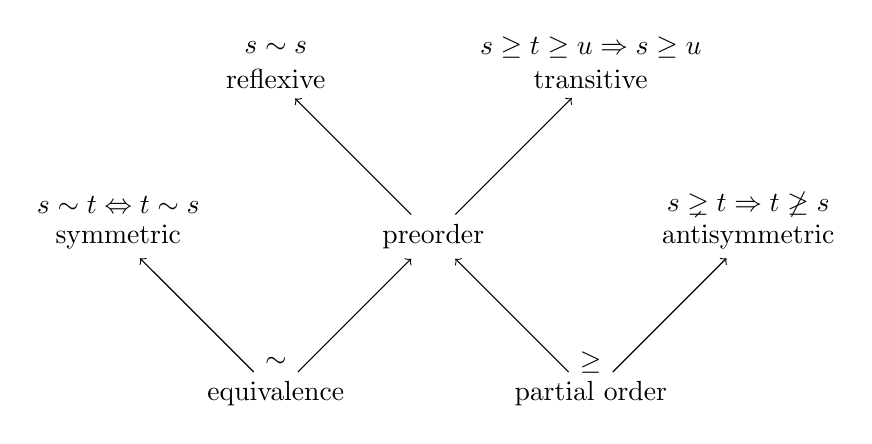
\begin{tikzpicture}

        \node (defSYMMETRIC) at (-4,0.4) { \( s\sim t\Leftrightarrow t\sim s \) };
        \node (SYMMETRIC) at (-4,0) { symmetric };

            \node (defREFLEXIVE) at (-2,2.4) { \( s\sim s \) };
            \node (REFLEXIVE) at (-2,2) { reflexive };

                \node (defTRANSITIVE) at (2,2.4) { \( s\geq t\geq u\Rightarrow s\geq u \) };
                \node (TRANSITIVE) at (2,2) { transitive };

                    \node (defANTISYMMETRIC) at (4,0.4) { \( s\gneq t \Rightarrow t\not\geq s \) };
                    \node (ANTISYMMETRIC) at (4,0) { antisymmetric };

        \node (PREORDER) at (0,0) { preorder };

    \node (SIM) at (-2,-1.6) { \( \sim \) };
    \node (EQUIVALENCE) at (-2,-2) { equivalence };

    \node (GEQ) at (2,-1.6) { \( \geq \) };
    \node (PARTIAL) at (2,-2) { partial order };

    % \node (PROPER) at (5,-1.5) { proper order };

    \draw[->] (PREORDER) -- (REFLEXIVE);
    \draw[->] (PREORDER) -- (TRANSITIVE);

    \draw[->] (EQUIVALENCE) -- (SYMMETRIC);
    \draw[->] (EQUIVALENCE) -- (PREORDER);
    \draw[->] (PARTIAL) -- (PREORDER);
    \draw[->] (PARTIAL) -- (ANTISYMMETRIC);

    % \draw[->] (PROPER) -- (TRANSITIVE);
\end{tikzpicture}
\end{figure}

\end{document}		% definitions and tikz macros
\usepackage[thinlines,thiklines]{easybmat}
%% ---------------------------------------------------------------------- %%

%% -- Macros ------------------------------------------------------------ %%
%% https://en.wikibooks.org/wiki/LaTeX/Macros
\usepackage{xspace}
% !TeX encoding = UTF-8

%% ==============================================================
%% ### MY MATH ENVIRONMENTS ###

\theoremstyle{plain}
%\newtheorem{theorem}{Theorem}			% predefined in CL?
%\newtheorem{proposition}{Proposition}	% predefined in CL?
%\newtheorem{lemma}{Lemma}				% predefined in CL?
%\newtheorem*{corollary}{Corollary}		% predefined in CL?

\theoremstyle{definition}
%\newtheorem{definition}{Definition}	% predefined in CL?
\newtheorem{conjecture}{Conjecture}
%\newtheorem*{example}{Example}			% predefined in CL?
%\newtheorem{algorithm}{Algorithm}		% predefined in CL
\newtheorem{procedure}{Procedure}
\newtheorem{goal}{Goal}
\newtheorem{notation}{Notation}

\theoremstyle{remark}
\newtheorem*{remark}{Remark}			% predefined in CL?
\newtheorem*{observation}{Observation}
%\newtheorem*{note}{Note}
%\newtheorem{case}{Case}

%% ==============================================================
%% ### MY MATH DEFINITIONS ###

% math alphabets

\DeclareMathAlphabet{\mathpzc}{OT1}{pzc}{m}{it}	% \mathpzc
\DeclareMathAlphabet{\mathcll}{T1}{calligra}{m}{n}

% math operators

\DeclareMathOperator{\arity}{arity}		% arity of a symbol

\DeclareMathOperator{\var}{\mathpzc{Vars}}			% variables of a term
\DeclareMathOperator{\fun}{\mathpzc{Funs}}			% function symbols of a term
\DeclareMathOperator{\pos}{\mathpzc{Pos}}			% positions in a term
\DeclareMathOperator{\posT}{\mathpzc{{t-}Pos}}			% positions in a term
\DeclareMathOperator{\posS}{\mathpzc{Pos^F}}
\DeclareMathOperator{\fvar}{\mathpzc{Fvars}}
\DeclareMathOperator{\bvar}{\mathpzc{Bvars}}

\DeclareMathOperator{\domain}{dom}			% domain of an assignment
\DeclareMathOperator{\range}{rng}		% range of an assignment
\DeclareMathOperator{\image}{img}			% image of an assignment

\DeclareMathOperator{\mgu}{mgu}			% most general unifier
\DeclareMathOperator{\sel}{sel}			% selection function

%\DeclareMathOperator{\mul}{mul}
%\DeclareMathOperator{\add}{add}
\DeclareMathOperator{\head}{head}
\DeclareMathOperator{\tail}{tail}
\DeclareMathOperator{\length}{length}



\DeclareMathOperator{\UNIF}{unifiable}
\DeclareMathOperator{\INST}{instance}
\DeclareMathOperator{\GNRL}{generalization}
\DeclareMathOperator{\VRNT}{variant}
\DeclareMathOperator{\PSTR}{pstr}

%\DeclareMathOperator{\subterms}{\mathpzc{Subterms}}	
%\DeclareMathOperator{\termsize}{size}
%\DeclareMathOperator{\symbols}{symbols}
%\DeclareMathOperator{\subforms}{\mathpzc{Subforms}}	
% !TeX encoding = UTF-8

% shortens the definition by cases
\newcommand{\DEFINE}[3][=]{{
		\begin{gather*}
		#2 #1 \left \{
				\begin{array}{ll}
					#3
				\end{array}
		\right.
		\end{gather*}
	}}


% accepts greek as input
\newcommand{\textgreek}[1]{\begingroup\fontencoding{LGR}\selectfont#1\endgroup}

\newcommand{\tikzmark}[1]{\tikz[overlay,remember picture] \node (#1) {};}


		% complex macros
\documentclass[]{clseminar}

    \documentclass[]{clseminar}

    \input{../PREAMBLE/Symbols}
    
    \begin{document}
    
    \author{Alexander Maringele}
    \title{Symbols}
    \abstract{The quick brown fox jumps over the lazy dog.
    Why?}
    
    \maketitle

    \newcommand{\demo}[1]{$#1$}

    \begin{itemize}
        \item \verb+\myem+ \myem The quick brown fox jumps over the lazy dog
        \item 
        \demo{\disjointunion},,
        \verb+\disjointunion+ 
        $\disjointunion$, 
        \verb+\false+ 
        $\false$,
        \verb+\lbic+ 
        $\lbic$,  
        \verb+\limp+ 
        $\limp$,  
        \verb+\succG\succL\succC+
        $\succG$,   
        \verb+\succG\succL\succC+
        $\succL$,   
        \verb+\succG\succL\succC+
        $\succC$, 
        \verb+\true+ $\true$

    \end{itemize}



    
        
    \end{document}
    
    \begin{document}
    
    \author{Alexander Maringele}
    \title{Symbols}
    \abstract{The quick brown fox jumps over the lazy dog.
    Why?}
    
    \maketitle

    \newcommand{\demo}[1]{$#1$}

    \begin{itemize}
        \item \verb+\myem+ \myem The quick brown fox jumps over the lazy dog
        \item 
        \demo{\disjointunion},,
        \verb+\disjointunion+ 
        $\disjointunion$, 
        \verb+\false+ 
        $\false$,
        \verb+\lbic+ 
        $\lbic$,  
        \verb+\limp+ 
        $\limp$,  
        \verb+\succG\succL\succC+
        $\succG$,   
        \verb+\succG\succL\succC+
        $\succL$,   
        \verb+\succG\succL\succC+
        $\succC$, 
        \verb+\true+ $\true$

    \end{itemize}



    
        
    \end{document}			% simple macros
%% ---------------------------------------------------------------------- %%

\usepackage{epigraph}


	% \usepackage{mystyle}
\newglossaryentry{Arithmetic}{name=Arithmetic,description={arithmetic}}
\newglossaryentry{Natural Deduction}{name=Natural Deduction, description={natural deduction}}

\makeglossaries

\makeindex

%\includeonly{
%%	introduction/introduction,
%	preliminaries/preliminaries,
%%	proving/proving,
%%	epr/epr,
%%	flea/flea,
%%	conclusion/conclusion,
%%	appendix/main
%}

\begin{document}
% \nocite{*}

% BEGIN: titlepage setup -------------------------------------------
\title{Yet another instantiation based\\first order theorem prover with equality}
\plaintitle{Theorem proving with equality}
\mailaddress{alexander.maringele@uibk.ac.at}
\matriculationnumber{8517725}
\author{Alexander~Maringele}
\plainauthor{Alexander~Maringele}
\date{\today}
\supervisor{Assoc.~Prof.~Dr.~Georg~Moser}
\institute{Institute of Computer Science}

\abstract{Instantiation-based \ldots}
% END: titlepage setup ----------------------------------------------

\acknowledgments{Thanks.!}
\maketitle
\tableofcontents

%====================================================================
% BEGIN: CONTENT ----------------------------------------------------
%====================================================================

\include{CONTENT/introduction} 		% ε
% !TeX root = ../mthesis.tex
% !TeX encoding = UTF-8
% !TeX spellcheck = en_US

\chapter{Preliminaries}





\epigraph{
	A good theory starts 
	
	with a good definition
}{
	unknown
}

We assume familiarity with propositional and predicate logic \cite{Huth:2004:LCS:975331}, 
automated theorem proving \cite{Fitting:1996:FLA:230183}, 
term rewriting \cite{Baader:1998:TR:280474}, 
decision procedures \cite{Kroening:2008:DPA:1391237}, 
and (maximum) satisfiability testing \cite{Biere:2009:HSV:1550723}.
Even so, for clarity we introduce basic
definitions and state basic lemmas and theorems without proofs.
This section is an extension of the same section in our seminar report \cite{axm:SR2}
where notions and notations largely follow those in lecture notes \cite{AM2015tr} and \cite{GM2013ar}.


\section{Syntax}

% !TeX root = ../mthesis.tex
% !TeX encoding = UTF-8
% !TeX spellcheck = en_US

\begin{definition}\label{def:signature}
A
first order
{\myem signature} with equality
%with equality
$\mcF = \mcFfPE$
is the disjoint union of
a set of {\myem function symbols} $\mcFf$,
a set of {\myem predicate symbols} $\mcFP$,
and one distinct equality symbol.
%
The {\myem arity} of a symbol determines the number of its arguments in a first order expression.
With $\mcFn = \{ \mcf\in\mcF \mid \arity(\mcf) = n \}$ we denote symbols with arity $n$.
\end{definition}

\begin{remark}
    We use $\mEQ$ as equality symbol in our signatures to emphasize
    that at this point it is just a highlighted symbol
    without “meaning”.
    On the other hand we use $=$ to express “identity” of objects
    like formualae or sets
    without actually defining how this identity can be determined.
\end{remark}


% !TeX root = ../mthesis.tex
% !TeX encoding = UTF-8
% !TeX spellcheck = en_US

\begin{definition}
	We build the set of (function) {\myem terms} $\mcTfFV$ 
	from function symbols $\mcFf \subseteq \mcF$ and 
	a countable set of {\myem variables} $\mcV$ disjoint from $\mcF$.
	Every variable $x\in\mcV$ is a term,
	every constant $c\in\mcFf^{(0)}$ is a term, 
	and every expression $f(t_1,\ldots,t_n)$
	for every function symbol $f\in\mcFf$ 
	with arity $n>0$ 
	and terms $t_1,\ldots,t_n$
	is a term.
%	
	We build the set of predicate terms or {\myem atoms} $\mcTPFV$
	from predicate symbols $\mcFP \subseteq \mcF$ and terms $t\in\mcTfFV$. 
	Every proposition $p\in\mcFP^{(0)}$ is an atom 
	and every expression $P(t_1,\ldots,t_n)$
	for every predicate symbol $P\in\mcFP$ with arity $n>0$ and terms $t_1,\ldots,t_n$ is an atom.
%	Every equation $s\ \mEQ\ t$ for terms $s,t$ is an atom too.
%
%	We speak of the set of general terms 
%	$\mcTFV = \mcTfFV\disjointunion\mcTPFV$ as the disjoint union of terms and atoms.
\end{definition}



% !TeX root = ../mthesis.tex
% !TeX encoding = UTF-8
% !TeX spellcheck = en_US

\begin{definition}\label{def:predicates}\label{def:equations}\label{def:atoms}
	We build the set of (first order) {\myem predicates} $\mcPT$
	from predicate symbols and terms.
	Every proposition $\mpp\in \mcFPn[0]$ is a predicate,
	and every expression $\mP(t_1,\ldots,t_n)$ is a predicate for $n>0$,
	predicate symbol $\mP\in\mcFPn$ and arbitrary terms $t_1,\ldots,t_n$.
%
	We build the set of (first order) {\myem equations }$\mcET$ from the equality symbol and terms.
	Every pair $s\mEQ t$ is an equation %\footnote{
%		We use prefix and infix notation interchangeable,
%		e.g.~${\mEQ}(s,t)$ represents the same equation as $s\mEQ t$.}
	for arbitrary terms $s$ and $t$.
%
	The set of atomic formulas (or {\myem atoms} for short) is the (distinct) union of predicates and equations.
\end{definition}

\input{preliminaries/ground}

% !TeX root = ../mthesis.tex
% !TeX encoding = UTF-8
% !TeX spellcheck = en_US

\begin{definition}[\index{FOF}\FOF]\label{def:syntax:FOF}
	Atoms from the previous definition are {\myem first order formulae}.  
	The universal quantification $(\forall x F)$ 
	and the existential quantification $(\exists x F)$ 
	of a first order formula are (quantified) first order formulae
	with {\myem bound} variable $x\in\mcV$.
	The negation $(\lnot F)$ of a first order formula
	is a (composite) first order formula.
	Further, the disjunction $(F \lor F')$, 
	the conjunction $(F \land F') $, 
	and the implication $(F \limp F')$ 
	of two first order formulae
	are (composite) first order formulae.
\end{definition}

\begin{definition}\label{def:term:vars}\label{def:fof:fvars}\label{def:fof:sentence}
	We define the set of variables of a first order term $t$ and the set of {\myem free} variables of a first order formula $F$ as follows:
\DEFINE{\var(t)} {
		\{ x \} & \text{if } t = x \in \mcV \\
		\bigcup_{i=1}^n \var(t_i) & \text{if }  t = \mf(t_1, \ldots t_n)
	}
\DEFINE{\fvar(F)}{
		\bigcup_{i=1}^n \var(t_i) &\text{if }F = \mP(t_1,\ldots,t_n)\text{ or }t_1\mEQ t_{n=2} 
		\\
		\fvar (G) \setminus \{ x\} &\text{if } F \in\{\, \forall x\,G, \exists x\,G\,\}
		\\
		\fvar(G) \cup \fvar(H)&\text{if }F \in\{\,G\land H,G\lor H,G\limp H\,\}
%		\\
%		\var(s) \cup \var(t) &\text{if }F = s\mEQ t
		\\
		\fvar(G)&\text{if }F = \lnot G
	}
\end{definition}

\begin{definition}\label{def:fof:closed}
	A closed first order formula or in other words
	a first order {\myem sentence} 
	is a first order formula without free variables,
	i.e.~all occurring variables are bound.
	\DEFINE{\bvar(F)}{
		\emptyset &\text{if }F = \mP(t_1,\ldots,t_n)\text{ or }t_1\mEQ t_{n=2} 
		\\
		\bvar (G) \cup \{ x\} &\text{if } F \in\{\, \forall x\,G, \exists x\,G\,\}
		\\
		\bvar(G) \cup \bvar(H)&\text{if }F \in\{\,G\land H,G\lor H,G\limp H\,\}
		%		\\
		%		\var(s) \cup \var(t) &\text{if }F = s\mEQ t
		\\
		\bvar(G)&\text{if }F = \lnot G
	}
\end{definition}

%\begin{remark} 
	We often will write formulae or sentences 
	without stating the first order signature.
The reader can easily deduce the underlying {\myem implicit} signature with arities 
and the set of variables by applying the definitions of the syntax for first order formulae.
We follow the convention to use $x,y,z$ for variables 
and $\ma,\mb,\mc$ for constant function symbols 
(which avoids ambiguity in the presence of free variables). 
For easier readability we will use uppercase predicate symbols and lowercase function symbols.
%\end{remark}

% !TeX root = ../mthesis.tex
% !TeX encoding = UTF-8
% !TeX spellcheck = en_US

\begin{definition}\label{def:literals}
A {\myem literal} $L$ is either an atom
or the negation of an atom.
%, where $l\not{}\hspace{-0.5mm}\circ$ abbreviates $\lnot(l\circ r)$
%for binary symobl $\circ$.
%A literal is ground if all its terms are ground.
%The complement $L^c$ of a literal $L$ is defined as %with some atom $A$: 
%\[ L^c = \left\{ \begin{array}{rl}
%A & \text{if } L = \lnot A\\
%\lnot A & \text{if } L = A
%\end{array}\right.
%\]
Two literals are complementary if one is an atom and the other is the negation of this atom.
%
A {\myem clause}\ \ $\mcC = L_1\lor\ldots\lor L_n$  is a possible empty multiset of literals 
and is equivalent to the universally quantified disjunction of its literals.
The {\myem empty clause} $\emptyclause$ expresses a contradiction. 
%A clause is ground if all its literals are ground.
A finite {\myem set of clauses} $S=\{ \mcC_1,\ldots,\mcC_n \}$ 
is equivalent to the conjunction of its clauses.
$S\equiv(\forall\vec{x}_1\mcC_1)\land\ldots\land(\forall\vec{x}_n\mcC_n)$ with 
$\vec{x}_i = \var(\mcC_i)$.
%$\vec{x}_i\cap\vec{x}_j=\emptyclause\lor i=j$.
%A set of clauses is ground if all its clauses are ground.
\end{definition}

% !TeX root = ../mthesis.tex
% !TeX encoding = UTF-8
% !TeX spellcheck = en_US

\begin{definition}\label{def:substitution}
	A {\myem substitution} $\sigma$ is a mapping from variables $x\in\mcV$ to terms in $\mcTFfV$
	where the {\myem domain }$\dom(\sigma) = \{ x\in\mcV\mid\sigma(x) \neq x \}$ is finite.
	We write substitutions as bindings $\sigma=\{ x_1\mapsto s_1,\ldots,x_n\mapsto s_n \}$
	where $\dom(\sigma)=\{ x_1,\ldots,x_n \}$ and $\sigma(x_i)=s_i$.
	A {\myem variable substitution} is a mapping from $\mcV$ to $\mcV$.
	A {\myem renaming} is a bijective variable substitution.
	A {\myem proper instantiator} is a substitution that is not a variable substitution.
	We define the instance $\mkt\sigma$ of a term, literal or clause $\mkt$,
	respectively the application of a substitution $\sigma$ to terms, literals, and clauses as follows:
	\begin{align*}
		\mkt\sigma &= \left\{\begin{array}{ll}
			s_i 					& \text{if }T=x_i\in\dom(\sigma)\\
			y					& \text{if }T=y\in\mcV\,\backslash\dom(\sigma)\\
%			c					& \text{if }tc \in \mcFf^{\!0}\\
			f(t_1\sigma,\ldots,t_n\sigma)	&\text{if }T=f(t_1,\ldots,t_n), f\in\mcFfn \\[0.5em]
			P(t_1\sigma,\ldots,t_n\sigma)	&\text{if }T=P(t_1,\ldots,t_n), P\in\mcFPn \\
			s\sigma\mEQ t\sigma			&\text{if }T=s\mEQ t \\[0.5em]
			\lnot(A\sigma)					&\text{if }T=\lnot A \\
			L_1\sigma\lor\ldots\lor L_n\sigma	&\text{if }T=L_1\lor\ldots\lor L_n \\
		\end{array}\right.	
	\end{align*}
%	
	We define the {\myem composition} of two substitutions $\sigma$ and $\tau$ as follows
	\begin{align*}
		\sigma\tau&=\{ x_i\mapsto s_i\tau\mid x_i\in\dom(\sigma) \}
		\cup
		\{ y_i\mapsto t_i\mid y_i\in\dom(\tau) \backslash \dom(\sigma) \}.
	\end{align*}
	
\end{definition}

\begin{lemma}\label{lem:substitution}
	With the definitions in \ref{def:substitution} the identity
%	$(\mkt\sigma)\tau = \mkt(\sigma\tau)$ holds for
	arbitrary terms, literals, clauses, and substitutions.
\end{lemma}

% !TeX root = ../mthesis.tex
% !TeX encoding = UTF-8
% !TeX spellcheck = en_US

\begin{definition}\label{def:unifier}
Two terms $s$ and $t$ are {\myem unifiable} if there exists a substitution $\sigma$ such that $s\sigma=t\sigma$.
They are {\myem variants} if their most general unifier is a renaming.
The {\myem most general unifier} $\sigma=\mgu(s,t)$ is a unifier such that
for every other unifier $\sigma'$ there exists a substitution $\tau$ such that
$\sigma' = \sigma \tau$. 
\end{definition}

\section{Semantics}

In this section we recall some basic aspects and definitions of semantics in first order logic. 
We state satisfiability of clauses. For brevity we ignore arbitrary formulas in first order logic
in our definitions.

\begin{definition}
	An {\myem interpretation} $\mcI$ over a signature $\mcF$ consists of a
	non-empty set $A$ -- the {\myem universe} or {\myem domain},
	definitions of (partial) functions $\mf_\mcI: A^n\rightarrow A$ for every function symbol $\mf\in\mcFf$, 
	and definitions of (possibly empty) n-ary relations 
	 ${\mP_\mcI}\subseteq A^n$ for every predicate symbol $\mP\in\mcFP$
	 and the definition of a binary relation ${\mEQ_\mcI}\subseteq A^2$ for the equality symbol.
	 An {\myem equational} interpretation defines $\mEQ_\mcI$ as equality on its domain.
	 i.e.~a ground term $s \mEQ_\mcI t$ holds if and only if $s_\mcI = t_\mcI$.
	
	A ground predicate $\mP(t_1,\ldots,t_n)$ {\myem holds} in interpretation $\mcI$ 
	if and only if $(t_1,\ldots,t_n) \in \mP_\mcI$.
	A ground literal does not hold in $\mcI$ if and only if its complementary literal holds in $\mcI$.
%	
	A non-ground literal holds in $\mcI$ if all its 
	(perhaps infinitely many) ground
	instances hold in $\mcI$.
	A clause holds in $\mcI$ if at least one of its literals holds in $\mcI$.
	A set of clauses $S$ holds in $\mcI$ if every clause $\mcC\in S$ holds in $\mcI$.
	We say $\mcI$ is a model {\em for} $S$ if $S$ holds in $\mcI$. 
	
	
\end{definition}

\begin{definition}
	A set of clauses $S$ is {\myem satisfiable} if and only if there is a model $\mcM$ for $S$. 
	A set of clauses is  {\myem valid} if and only if all clauses hold in every interpretation.
\end{definition}

\begin{definition}\label{def:hk}
	An {\myem Herbrand universe} is the smallest set of terms that contains all $H_k\ge 0$ of
	\begin{align*}
	H_0 &:= \left\{ 
	\begin{array}{ll}
	\{ \mc \mid \mc\in\mcFfn[0] \} 
	&\text{if } \mcFfn[0]\not=\emptyset\\
	\{ \mc \}
	&\text{if } \mcFfn[0]=\emptyset, \mc\not\in\mcF
	\end{array}
	\right. 
	\\
	H_{k+1} &:= H_k \cup \{\  
	\mf(t_1,\ldots,t_n) \mid
	\mf\in\mcFfn[n],
	t_1,\ldots,t_n \in H_k
	\ \}
	\end{align*}
	
\end{definition}

\begin{definition}
	An {\myem Herbrand interpretation} $\mcH$ is an interpretation where the domain 
	is an Hebrand universe
	and the interpretation of each ground term $t_\mcH := t$ is the term itself.
\end{definition}

\begin{example}
	Consider the satisfiable set of clauses 
	$S = \{  
		\mP(\mf(x)) 
	\}$. 
	Let $H_S = \{ 
		\mc, \mf(\mc), \mf(\mc), \ldots, \mf^i(\mc), \ldots
	\}$ be the Hebrand universe for $S$.
	We define $\mf_I$ by mapping $\mc_I := \mc$,
	$\mf_I^{i+1}(x) := \mf (\mf_I^i(x))$
\end{example}

\begin{definition}
	An {\myem term interpretation} 
	$\mcI_t$ 
	is an interpretation 
	where the elements of its domain $A = \mcTFf/_\sim$ 
		are equivalence classes of ground terms
		and the interpretation of each ground term $t^{\mcI_t} := [t]_\sim$ is its equivalence class.
%		An equation $s\mEQ t$ of ground terms holds in if $[s]_\sim=[t]_\sim$.
	 A ground predicate $\mP(t_1,\ldots,t_n)$ holds if 
	 $([t_1]_\sim,\ldots,[t_n]_\sim) \in \mP^{\mcI_t} \subseteq A^n$.
%	A ground literal does not hold if and only if its complementary literal holds.
	In an {\myem equational} term interpretation an equation $s\mEQ t$ holds if an only if $s\sim t$.
	
\end{definition}

\begin{example}
	Consider the satisfiable set of clauses $S = \{ x \mEQ \mf(x) \}$. 
%	
	We easily find a Herbrand model $\mcH$ with
	predicate definition $\mEQ^\mcH = \{ (\mf^{i}(\ma)), \mf^{i+1}(\ma)) \mid i\geq 0  \} $. 
	However $\mcH$ is not an equational model because obviously $\ma\neq\mf(\ma)$ in its domain.
%	
	Further on we easily find an equational model $\mcM$ 
	with domain $\{ \mc \}$, function definition $\mf^\mcM(\mc) = \mc$, 
	and $\mEQ_\mcM$ is defined by equality in its domain.
	Certainly this model $\mcM$ is not an Hebrand model 
	because the interpretation of ground term ${\mf(\mc)}^\mcM \neq \mf(\mc)$ is not the term itself.
	
	On the other hand we easily get an equational term model with domain $\{ [\ma]_\sim\}$, 
	a plain function definition
	$\mf([\ma]_\sim) = [\ma]_\sim$, 
	and an equivalence relation
	$\ma \sim \mf(\ma)$
	where $\mEQ$ is defined by equality in its domain.	
\end{example}


%\section{Term Rewriting}
%
%
%
%
%\begin{definition}
%	A {\myem rewrite rule} is an equation of terms where the left-hand side is not a variable
%	and the variables occuring in the right-hand side occur also in the left-hand side.
%	%	\[
%	%		\ell\rwEQ r \text{ is rewrite rule }\quad :\Longleftrightarrow\quad\ell\not\in\mcV\text{ and }\var(r)\subseteq\var(l)
%	%	\] 
%	A rewrite rule $\ell'\rwEQ r'$ is a {\myem variant} of $\ell\rwEQ r$ if there is a renaming $\varrho$
%	such that 
%	$(l\rightarrow r)\varrho = l'\rightarrow r'$.
%	A {\myem term rewrite system} is a set of rewrite rules without variants.
%\end{definition}
%
%\begin{definition}\label{def:position}
%	A {\myem position} is a finite sequence of positive integers.
%	The root position is the empty sequence $\epsilon$.
%	The position $pq$ is obtained by concatenation of positions $p$ and $q$.
%	%
%	The set of all positions of an expression $\mct$ is defined as 
%	\DEFINE{ 
%		\pos(\mct) }
%	{
%		\{ \epsilon \} 		
%		& \text{if }\mct = x \in \mcV \\
%%		
%		\{ \epsilon \} \cup \bigcup_{i=1}^{n} \{ iq\mid q\in\pos(t_i) \}	
%		& \text{if }\mct=\mcf(t_1,\ldots,t_n)\text{ where } \mcf\in\mcF^{(n)}.
%	}
%The~{\myem subexpression} $\mct|_p$ of an expression $\mct$ {\myem at position} $p\in\pos(\mct)$ is defined as
%%
%\DEFINE{
%	t|_p
%}{
%	t 		& \text{if }p=\epsilon \\
%	t_i|_q	& \text{if }t=\mcf(t_1,\ldots,t_n)\text{ and }p=iq
%}
%%
%If $s$ is an expression then $t[s]_p$ represents the expression build by replacing the subexpression of $t$ at position $p$ with the term $s$.
%\DEFINE{
%	t[s]_p}
%{
%	s 		& \text{if }p=\epsilon \\
%	\mf(t_1,\ldots,t_i[s]_q,\ldots,t_n)	& \text{if }t=\mf(t_1,\ldots,t_n)\text{ and }p=iq
%}
%%A {\myem hole} denotes a special constant symbol $\ctxhole\in\mcFf^{(0)}$. 
%%A {\myem context} is a term $t$ with exactly one hole, i.e.~one occurrence $|t|_{\ctxhole}=1$.
%\end{definition}
%
%\begin{definition}
%	We say $s\rightarrow_\mcR t$ is a 
%	{\myem rewrite step} 
%	 with respect to TRS $\mcR$ 
%	when there is a position $p \in \pos(s)$, 
%	a rewrite rule $l\rwEQ r\in\mcR$, 
%	and a substitution $\sigma$ such that
%	$s|_p=l\sigma$ and $s[r\sigma]_p = t$.
%		The subterm $l\sigma$ is called {\myem redex} and
%	$s$ rewrites to $t$ by {\myem contracting} $l\sigma$ to {\myem contractum} $r\sigma$.
%	%
%	We say a term $s$ is {\myem irreducible} or in {\myem normal form} with respect to TRS $\mcR$ if there is no rewrite step $s\rightarrow_\mcR t$ for any term $t$. 
%	The set of normal forms $\mNFR$ contains all irreducible terms of the TRS $\mcR$.
%	\end{definition}
%
%%\begin{definition}
%%	A {\myem rewrite relation} is a binary relation on terms that is closed under contexts and substitutions.
%%	A {\myem rewrite order} is a proper order (i.e. irreflexive and transitive relation) and a rewrite relation.
%%	A {\myem reduction order} is a well-founded rewrite order.
%%\end{definition}
%
%\begin{definition}
%	A term $s$ can be rewritten to term $t$ with notion $s\rightarrow^*_\mcR t$ 
%	if there exists at least one {\myem rewrite sequence} $(a_1,\ldots ,a_n)$ such that
%	$s=a_1$, $a_n=t$, and $a_i\rightarrow_\mcR a_{i+1}$ are rewrite steps for $1\leq i<n$.
%	A TRS is {\myem terminating} if there is no infinite rewrite sequence of terms.
%	%
%	Two Terms $s$ and $t$ are {\myem joinable} with notion $s\downarrow t$ 
%	if both can be rewritten to some term $c$, i.e.~$s \rightarrow^*c\ \, ^*\!\!\leftarrow t$.
%%	
%	Two Terms $s$ and $t$ are {\myem meetable} with notion $s\uparrow t$ 
%	if both can be rewritten from some common ancestor term $a$, i.e.~$s \leftarrow^*a\ \, ^*\!\!\rightarrow t$.
%%
%	A TRS is {\myem confluent } if $s$ and $t$ are joinable whenever $s\ ^*\!\!\leftarrow a \rightarrow^* t$ holds for some term $a$.
%	%
%	Terms $s$ and $t$ are {\myem convertible} with notion $s\leftrightarrow^* t$ 
%	if there exists a sequence $(a_1,\ldots ,a_n)$ such that
%	$s=a_1$, $a_n=t$, and $a_i\leftrightarrow a_{i+1}$, i.e.~$a_i\rightarrow a_{i+1}$ or $a_i\leftarrow a_{i+1}$ are rewrite steps for $1\leq i<n$.
%\end{definition}
%
%\begin{definition}\label{def:closed-under}
%	A {\myem rewrite relation} is a binary relation $\relation$ on terms thats is {\myem closed under contexts},
%	i.e.~$u[s]_p\relation u[t]_p$ %holds 
%	for all positions $p\in\pos(u)$ and
%	for all terms $s,t,u$ whenever $s\relation t$
%	and {\myem closed under substitutions}, 
%	i.e.~$s\sigma\relation t\sigma$ %holds
%	for all substitutions $\sigma$
%	and all terms $s,t$ whenever $s\relation t$.
%\end{definition}
%\begin{lemma}
%	The relations $\rightarrow^*_\mcR$, 
%	$\rightarrow^+_\mcR$,
%	$\downarrow_\mcR$, $\uparrow_\mcR$ are rewrite relations on every TRS $\mcR$.
%\end{lemma}
%%
%\begin{definition}
%	A proper (i.e.~irreflexive and transitive) order on terms is called {\myem rewrite order} if it is a rewrite relation.
%	A {\myem reduction order} is a well-founded rewrite order,
%	i.e.~there is no infinite sequence 
%	$(a_i)_{i\in\mathbb{N}}$
%	where $a_i\gtpre a_{i+1}$ for all $i$.
%	% with $i\in\mathbb{N}$.
%	A {\myem simplification order} is a rewrite order with the {\myem subterm property},
%	i.e.~$u[t]_p \gtpre t$ for all terms $u$, $t$ and positions $p\neq\epsilon$.
%\end{definition}
%\begin{lemma}
%	Every simplification order is well-founded, i.e.~it is a reduction order.
%\end{lemma}
%%% DEF %%
%%
%\begin{theorem}
%	A TRS $\mcR$ is terminating if and only if there exists a reduction order $\gtpre$
%	such that $l\gtpre r$ for every rewrite rule $l\rightarrow r\in\mcR$.
%	We call $\mcR$ simply terminating if $\gtpre$ is a simplification order.
%\end{theorem}

\section{Usefull theorems}

\begin{theorem}[Church 1936, Turing 1937]
The satisfiability problem for first order logic is undecidable
\end{theorem}

\begin{theorem}[Compactness]\label{the:compactness}
	If every finite subset of a set of formulas $S$ has a model then $S$ has a model. 
\end{theorem}

\begin{theorem}[Löwenheim Skolem]\label{the:loewenheim}
	If a set of formulas $S$ has a model then $S$ has a countable model.
\end{theorem}

\begin{theorem}[Herbrand]\label{the:herbrand}
	Let $S$ be a set of clauses without equality. Then the following statements are equivalent.
	\begin{itemize}
		\item $S$ is satisfiable.
		\item $S$ has a Herbrand model.
		\item Every finite subset of all ground instances of $S$ has a Herbrand model.
	\end{itemize} 
\end{theorem}

\begin{corollary}
	Let $S$ be a set of clauses without equality. 
	Then $S$ is unsatisfiable if and only if there exists 
	an unsatisfiable finite set of ground instances of $S$.
\end{corollary}

%\section{Conventions}
%
%\begin{align*}
%\mc, \md &\ \in\mcFfn[{0}]\tag*{constant symbols} \\
%\mf, \mg, \mh &\ \in\mcFfn[{n>0}]\tag*{function symbols} \\
%\mpp, \mq, \mr &\ \in\mcFPn[{0}]\tag*{propositional symbols}\\
%\mP, \mQ, \mR &\ \in\mcFPn[{n>0}]\tag*{predicate symbols}\\
%s,t,u &\ \in\mcTf = \mcTFfV\tag*{terms}
%\end{align*}


		% almost
% !TeX root = ../mthesis.tex
% !TeX encoding = UTF-8
% !TeX spellcheck = en_US


\chapter{Completeness and Undecidability}

We call a logical calculus, i.e.~a formal proof system for an underlying logic, 
{\myem complete} if every valid formula is provable.
In other words, any expression that is satisfied by all possible interpretations 
is deducible or justifiable by applying rules of the formal system only.
We expect a useful calculus to be {\myem sound}, that is, every proven formula is valid, 
i.e.~it holds in any interpretation.
We call a logical system {\myem decidable} 
if and only if a purely syntactical algorithm exists that determines 
the validity or non-validity for any arbitrary formula in the given logical system.
%A standard example for a decidable logic is propositional logic.

We first look at a sound and complete calculus for first-order logic in \ref{sec:natural:deduction}.
After that we recall undecidability of first-order logic in \ref{sec:decidable:fol:theorems} 
together with other useful theorems about first-order logic.
Then we enumerate decidable fragments of first-order logic
which can be described purely syntactically in \ref{sec:decidable:fol:fragments} .
After that we look at decidable first-order theories in \ref{sec:decidable:fol:theories}, 
which are not necessarily expressible 
in one of the syntactically describable and decidable fragments of first-order logic.

\section{\gls{Natural Deduction}}
\label{sec:natural:deduction}

In Natural Deduction \cite{Huth:2004:LCS:975331}
we start with a (possible empty) set of formulae -- the premises -- 
and infer other formulae -- the conclusions -- by using syntactic proof rules from Tables 
\ref{tab:natural:deduction:connectives}, \ref{tab:natural:deduction:equality}, 
and \ref{tab:natural:deduction:quantifiers}.
The symbols $F$ and $G$ in these rules represent arbitrary first-order formula 
as defined in Definition \vref{def:syntax:FOF}. 
We open a box when we assume something, e.g.~that $F$ holds. 
We close the box when we discard the assumption. 
With $F_1,\ldots,F_n \proves H$ we claim that formula $H$ 
is in the transitive closure of inferable formulae from $\{ F_1,\ldots,F_n\}$.
(e.g.~the natural deduction proof to Lemma \vref{lemma:equivalence:congruence}).

% !TeX root = ../mthesis.tex
% !TeX encoding = UTF-8
% !TeX spellcheck = en_US

In Tables \ref{tab:natural:deduction:connectives}, \ref{tab:natural:deduction:equality}, and \ref{tab:natural:deduction:quantifiers} 
the symbols $F$ and $G$ represent arbitrary first order formula as defined in Definition \vref{def:syntax:FOF}.  

\begin{table}[hbt]
\begin{gather*}
\begin{array}{ccccc}
\infer[(\land i)]{F\land G}{F & G} 
&
\infer[(\land e_1)]{G}{F \land G} 
&
\infer[(\land e_2)]{F}{F \land G}
&
\infer[(\lnot\lnot i)]{\lnot\lnot F}{F} 
&
\infer[(\lnot\lnot e)]{F}{\lnot\lnot F}
\\[0.7em]
\infer[(\bot e)]{F}{\bot}
&
\infer[(\lnot e)]{\bot}{F & \lnot F}
&
\infer[\text{LEM}]{F\lor\lnot F}{}
&
\infer[(\lor i_1)]{F\lor G}{F}
&
\infer[(\lor i_2)]{F\lor G}{G}
\\[0.7em]
\infer[(\lnot i)]{\lnot F}{
	\boxed{\begin{array}{c}F\\\vdots\\\bot\end{array}}}
&
\infer[\text{PBC}]{F}{
	\boxed{\begin{array}{c}\lnot F\\\vdots\\\bot\end{array}}}
&
\infer[({\limp} i)]{F\limp G}{
	\boxed{\begin{array}{c}F\\\vdots\\G\end{array}
}}
&
\multicolumn{2}{l}{
	\infer[(\lor e)]{H}{
		F\lor G &
		\boxed{\begin{array}{c}F\\\vdots\\H\end{array}} &
		\boxed{\begin{array}{c}G\\\vdots\\H\end{array}}
	}	
}
\\[0.7em]
&
\multicolumn{3}{r}{
\infer[\text{modus}\atop\text{ponens}]{G}{F & F\limp G}
\qquad
\infer[\text{modus}\atop\text{tollens}]{\lnot F}{F\limp G & \lnot G}
}
&
\end{array}
\end{gather*}
\caption{Natural Deduction Rules for Connectives}
\label{tab:natural:deduction:connectives}
\end{table}
\begin{itemize}
	\item[($\land i$)] If $F$ and $G$ hold we may introduce the conjunction $F\land G$.
	\item[($\land e$)] If $F \land G$ holds we may eliminate the conjunction and keep $F$ or $G$.
	\item[($\lnot\lnot$)] We may introduce or eliminate double negation at any time.
	\item[($\bot e$)] Ex falso sequitur quodlibet. 
	\item[($\lnot e$)] 
	\item[LEM] Tertium non datur. Law of excluded middle.
	\item[($\lor i$)] If $F$ or $G$ hold we may introduce the disjunction $F\lor G$.
	\item[($\lnot i$)] 
\end{itemize}

\begin{table}[hbt]
	\begin{gather*}
	\infer[({=}i)]{t=t}{}
	\qquad
	\infer[({=}e)]{F\{x\mapsto t\}}{s=t & F\{x\mapsto s\}}
	\end{gather*}
	\caption{Natural Deduction Rules for Equality}
	\label{tab:natural:deduction:equality}
\end{table}

\begin{table}[hbt]
	\begin{gather*}
	\begin{array}{ccc}
	\infer[(\forall e)]{F\{x\to t\}}{
		\forall x F
	}
	&&
		\infer[(\exists i)]{\exists x F}{
		F\{x\mapsto x_0 \}
	}
	\\[1em]
	\infer[(\forall i)]{\forall x F}{
		\boxed{\begin{array}{cc}x_0\\&\vdots\\&F\{x\mapsto x_0\}\end{array}}
	}
	&&
	\infer[(\exists e)]{H}{
		\exists x F &
		\boxed{\begin{array}{cc}x_0&F\{x\mapsto x_0 \}\\&\vdots\\&H\end{array}}
	}
	\end{array}
	\end{gather*}
	\caption{Natural Deduction Rules for Quantifiers}
	\label{tab:natural:deduction:quantifiers}
\end{table}

\begin{theorem}[Soundness]
	The inference rules of natural deduction are sound.
\end{theorem}

\section{Theorems of First Order Logic}\label{sec:decidable:fol:theorems}

The purpose of this section is to state useful theorems about first-order logic.

\begin{theorem}[Completeness, Gödel 1929]
	Natural deduction (see above), a sound formal system, is complete.
\end{theorem}

\begin{theorem}
	[Undecidability, Church 1936, Turing 1937]
	The satisfiability problem for first-order logic is undecidable.
\end{theorem}

\begin{theorem}[Trakhtenbort 1950, Craig 1950]
	The satisfiability problem for first-order logic on {\myem finite} structures (domains) is undecidable.
\end{theorem}

\begin{definition}[Finite model property]
	A logic has the finite model property if each non-theorem is falsified by some finite model.
\end{definition}

\begin{lemma}[Refutation]
	By definition of the semantics of negation a formula is valid if and only if its negation is not satisfiable.
\end{lemma}

\begin{theorem}[Compactness, Gödel 1930, Maltsev 1936]\label{the:compactness}
	If every finite subset of a set of formulas $S$ has a model then $S$ has a model. 
\end{theorem}

\begin{theorem}[Löwenheim Skolem, 1915, 1920]\label{the:loewenheim}
	If a set of formulas $S$ has a model then $S$ has a countable model.
\end{theorem}

\begin{theorem}[Herbrand, 1930]\label{the:herbrand}
	Let $S$ be a set of clauses without equality. Then the following statements are equivalent.
	\begin{itemize}
		\item $S$ is satisfiable.
		\item $S$ has a Herbrand model.
		\item Every finite subset of all ground instances of $S$ has a Herbrand model.
	\end{itemize} 
\end{theorem}

\begin{corollary}
	Let $S$ be a set of clauses without equality. 
	Then $S$ is unsatisfiable if and only if there exists 
	an unsatisfiable finite set of ground instances of $S$.
\end{corollary}

\begin{lemma}
With Skolemization and Tseitin transformation we can effectively transform a arbitrary first-order formula into an equisatisfiable set of clauses.	
\end{lemma}


\section{Decidable Fragments of First Order Logic}\label{sec:decidable:fol:fragments}

This section presents purely syntactical defined fragments
of first-order logic where satisfiability is decidable.\footnote{
	\,Definitions and compact overviews follow the presentation
	“\href{http://logic.rwth-aachen.de/~graedel/kalmar.pdf}{Decidable fragments of first-order and fixed-point logic}”
	by E.~Grädel (\url{http://logic.rwth-aachen.de/~graedel/}).	
}  



\begin{definition}[\PNF]
	A first-order formula $F = \quantify_1 x_1 \ldots \quantify_n x_n\, G$ 
	where $\quantify_i \in \{\exists,\forall\}$ are quantifiers
	for $1 < i \leq n$,
	the subformula $G$ is quantifier free, and 
	the set of free variables $\fvar(G) = \{ x_1, \ldots, x_n \}$
	matches the quantified variables
	is in {\myem prenex normal form}.
\end{definition}


\begin{definition}[\cite{MR1482227}]\label{def:prefix:class}
	We describe classes of first-order formulae in \PNF with triples
	\[
	[\, \Pi, (p_1,p_2,\ldots), (f_1,f_2,\ldots)\,]_{(\mEQ)} \subseteq [\, all, all, all\,]_{\mEQ}
	\]
	where $\Pi = \quantify_1 \ldots \quantify_n$, $\quantify_i\in\{\forall,\exists\}$ 
	describes the structure of the quantifier prefix (without variables) of the formulae,
	the value $p_i$ is the maximal number of predicate symbols with arity $i$,
	and the value $f_i$ the maximal number of function symbols with arity $i$ in the signature.
	The equality symbol is not counted as binary predicate symbol. Instead,
	the absence or presence of subscript $(\mEQ)$ indicates whether the equality symbol is in the signature. 
\end{definition}

\begin{example}\label{ex:monadic}
	The monadic predicate calculus includes formulae with arbitrary quantifier prefixes, 
	arbitrary many unary predicate symbols, the equality symbol, but no function symbols.
	\begin{gather*}
	{\colG [\,all, (\omega), (1)\,]_= 
	\quad\supsetneq}\qquad 
	[\,all, (\omega), (0 ) \,]_=
	\tag{Löwenheim 1925, Kalmár 1929}
	\end{gather*}
\end{example}

\begin{example}\label{ex:ackermann}
	The Ackermann prefix class contains formulae with arbitrary many existential quantifiers, 
	but just one universal quantifier. It contains arbitrary many predicate symbols
	with arbitrary arities, the equality symbol, but no function symbols. 
	\begin{gather*}
	{\colG [\,\exists^*\forall\exists^*,all,(1)\,]_=
	\quad\supsetneq}\qquad
	[\,\exists^*\forall\exists^*,all,(0) \,]_{=}\qquad\qquad\qquad 
	\tag{Ackermann 1928}
	\end{gather*}
\end{example}

\begin{remark}
	One unary function symbol can be added to these fragments of first order logic above 
	without loosing decidability (see Table \vref{tab:decidable:InfinityAxioms}).
\end{remark}

%Goldfarb, Gurevich, Rabin, Shelah completly characterized decidable and undecidable prefix classes.

\begin{table}[hbt]
	\begin{align*}
	%\colG [\,all, (\omega), (0 )&\colG\,]_= \tag{Löwenheim 1925, Kalmár 1929}
	%\\
	[\,\exists^{∗}\forall^{∗}, all, (0)&\,]_{=} \tag{Bernays, Schönfinkel 1928, Ramsey 1932}
	\\
	[\,\exists^{∗}\forall^2\exists^{∗} , all, (0)&\,] \tag{Gödel 1932, Kalmár 1933, Schütte 1934}
	\\
	[\,all, (\omega), (\omega)&\,] \tag{Löb 1967, Gurevich 1969}
	\\
	[\,\exists^{∗}\forall\exists^{∗}, all, all&\,] \tag{Gurevich 1973}
	\\
	[\,\exists^{∗}, all, all&\,]_{=} \tag{Gurevich 1976}
	\end{align*}
	%\caption[Decidable prefix classes]{Decidable prefix classes in first-order logic}
	\caption[Decidable prefix classes]{Decidable prefix classes with final model property }
	\label{tab:decidedable:FiniteModelProperty}
\end{table}

\begin{table}[hbt]
	\begin{align*}
	[\,all, (\omega), (1)&\,]_{=} \tag{Rabin 1969} 
	\\
	[\,\exists^{∗}\forall\exists^{∗}, all, (1)&\,]_{=} \tag{Shelah 1977}
	\end{align*}
	%\caption[Decidable prefix classes]{Decidable prefix classes in first-order logic}
	\caption[Decidable prefix classes]{Decidable prefix classes with infinity axioms. }
	\label{tab:decidable:InfinityAxioms}
\end{table}

\begin{lemma}
	Satisfiability is decidable \cite{MR1482227} in all prefix classes from Tables 
	\ref{tab:decidedable:FiniteModelProperty} and \ref{tab:decidable:InfinityAxioms}.
	Each of theses classes is closed under conjunction with respect to satisfiability.
\end{lemma}



\section{Theories in First Order Logic}\label{sec:decidable:fol:theories}

We follow definitions and examples in \cite{AM2015L}.

\begin{definition}[Theory]
	A {\myem first-order theory} is a pair of a first-order signature 
	and the possible infinite conjunction $\bigwedge_i A_i$ of first-order formulae, 
	i.e.~the axioms, over the theory's signature. 
	A theory is satisfiable if there exists a model for its axioms.
	A theory is consistent when the contradiction is not derivable.
%	
	A {\myem theorem} is a sentence over the theory's signature, 
	i.e.~a closed formula, that holds in any model for the theory's axioms.
	\[
		\bigwedge_i A_i \models \mathsf{theorem} 
		\quad\text{ or }\quad
		\bigwedge_i A_i \limp \mathsf{theorem} 
	\]
	A theory is decidable if it is decidable whether an arbitrary sentence holds in the theory.
\end{definition}

\begin{example}
A theory with axioms $\forall x\,\mP(x)$ and $\exists x\,\lnot\mP(x)$ is not satisfiable,
but every sentence is a theorem. Hence it is not consistent, too.
\end{example}
%
\begin{remark} 
In refuational theorem proving
we show the unsatisfiabilty 
of a negated sentence, 
i.e.~a {\myem conjecture},
in conjunction with the axioms
to conclude that the conjecture is indeed a theorem.
\[
	\lnot\left(\bigwedge_i A_i \limp \mathsf{conj}\right) \equiv
	\lnot\left(\lnot\bigwedge_i A_i \lor \mathsf{conj}\right) \equiv
	\bigwedge_i A_i \land \lnot \mathsf{conj}
\]
\end{remark}

In the following we define equivalence and congruence as usual. Together these axioms form the theory of equality.

\begin{definition}
	[Equivalence]
	\label{def:equivalence:axioms}
\begin{align*}
\forall x\, 
&\left(x \mEQ x\right) 
\tag*{reflexivity}
\\
\forall x \forall y\, 
&\left(x \mEQ y \limp y \mEQ x \right)
\tag*{symmetry} 
\\
\forall x \forall y \forall z\,
&\left(x \mEQ y \land y\mEQ z \limp x\mEQ z\right) 
\tag*{transitiviy}
\end{align*}
\end{definition}

\begin{definition}[$\vec{x}$-Notation]
	Occasionally we may abbreviate a sequence of $n$ variables by $\vec{x}$.
	Then we write $\mcf(\vecn{x})$ 
	for first-order expression $\mcf(x_1,\ldots,x_n)$
	with n-ary function or predicate symbol $\mcf$,
%	 $\mcf\in\mcFn$,
	a single equation $\vecn{x}\mEQ\vecn{y}$ for
	the conjunction of $n$ equations 
	$x_1\mEQ y_1\land\ldots\land x_n\mEQ y_n$,
	and $\forall\vecn{x}$ for 
	the sequence of quantified variables $\forall x_1\ldots\forall x_n$.
\end{definition}

\begin{definition}
	[Congruence schemata]
	\label{def:congruence:schemata}
	\begin{align*}
	\forall\vecn{x}\,\forall\vecn{y}\,
	&\left(\vecn{x}\mEQ\vecn{y} \limp \mf(\vecn{x}) \mEQ \mf(\vecn{y}) \right)
	\tag*{for all $\mf\in\mcFfn$}
	\\
	\forall\vecn{x}\,\forall\vecn{y}\, 
	&\left(\vecn{x}\mEQ\vecn{y} \limp (\mP(\vecn{x}) \limp \mP(\vecn{y}))\right)
	\tag*{for all $\mP\in\mcFPn$}
	\end{align*}
	
	
\end{definition}

%\begin{remark}For simplicity we have replaced biconditionals in symmetry and predicate congruence with implications.
%	\begin{align*}
%	\forall x \forall y\,
%	\left(x \mEQ y \lbic y \mEQ x \right) 
%	&
%	\equiv\forall x \forall y\,
%	\left(x \mEQ y \limp y \mEQ x \right)
%	\\
%	\forall\vec{x}\,\forall\vec{y}\, 
%	\left(\vec{x}\mEQ\vec{y} \limp (\mP(\vec{x}) \lbic \mP(\vec{y}))\right)
%	&\equiv
%	\forall\vec{x}\,\forall\vec{y}\,
%	\left(\vec{x}\mEQ\vec{y} \limp (\mP(\vec{x}) \limp \mP(\vec{y}))\right)
%	\end{align*}
%\end{remark}
%
\begin{lemma}\label{lemma:equivalence:congruence}
Equivalence and congruence of equality are provable by Natural Deduction (see Section \vref{sec:natural:deduction}).\end{lemma}
\begin{proof}
	For brevity we skip the quantifier introductions for symmetry, transitivity, and congruence.
	Additionally we just show congruence for a unary function and a unary predicate symbol.
	\begin{gather*}
\begin{BMAT}{rcrclccl}{cc}
1 && x_0 && x_0=x_0 	& && {=}i\\
2 && 	 &&	\forall x\,(x=x)	& && \forall{}i,1
\addpath{(2,1,1)rrrrulllld}
\end{BMAT}
\\
\begin{BMAT}{rcrclccl}{ccccccc}
1 && && y = y   & && {=}i\\
2 && && x = y	& && \texttt{assume}\\
3 && &&	y\neq x	& && \texttt{assume}\\
4 && && y\neq y & && {=}e,2,3\\
5 && && \bot    & && {\lnot}e,1,4 \\
6 && && y = x   & && \texttt{PBC}, 3{-} 5\\
7 && && x = y \limp y = x & && {\limp}i, 1{-} 5
\addpath{(2,1,1)rrrruuuuullllddddd}
\addpath{(3,2,1)rruuullddd}
\end{BMAT}
\qquad
\begin{BMAT}{rcrclccl}{ccccc}
1 &&     && x=y\land y=z 	& && \texttt{assume}\\
2 && 	 &&	y=z	& && \land{}e_2 \\
3 && 	 &&	x=y	& && \land{}e_1, 2 \\
4 && 	 &&	x=z	& && {=}e,2,3 \\
5 && 	 &&	x=y\land y=z\limp x=z	& && {\limp}i,2{-}4 
\addpath{(2,1,1)rrrruuuulllldddd}
\end{BMAT}
\\
\begin{BMAT}{rcrclccl}{ccccccc}
1 && && \mf(y) = \mf(y)   & && {=}i\\
2 && && x = y	& && \texttt{assume}\\
3 && &&	\mf(x) \neq \mf(y)	& && \texttt{assume}\\
4 && && \mf(y) \neq \mf(y) & && {=}e,2,3\\
5 && && \bot    & && {\lnot}e,1,4 \\
6 && && \mf(x) = \mf(y)   & && \texttt{PBC}, 3{-} 5\\
7 && && x = y \limp \mf(x) = \mf(y) & && {\limp}i, 1{-} 5
\addpath{(2,1,1)rrrruuuuullllddddd}
\addpath{(3,2,1)rruuullddd}
\end{BMAT}
\qquad
\begin{BMAT}{rcrclccl}{ccccc}
1 && && x = y	& && \texttt{assume}\\
2 && &&	\mP(x)	& && \texttt{assume}\\
3 && && \mP(y) & && {=}e,1,2\\
4 && && \mP(x) \limp \mP(y)   & && {\limp}i, 2{-} 3\\
5 && && x = y \limp (\mP(x)\limp\mP(y)) & && {\limp}i, 1{-} 4
\addpath{(2,1,1)rrrruuuulllldddd}
\addpath{(3,2,1)rruulldd}
\end{BMAT}
\end{gather*}
\end{proof}

\begin{definition}
	[Natural Numbers]
	\label{def:natural:numbers:axioms}
	We introduce a fresh constant $0\in\mcFn[0]$, 
	a unary successor symbol $\msucc\in\mcFn[1]$,
	and restrict their models with two axioms. 
\begin{align*}
\forall x\, &(\msucc(x) \mNE 0)
\tag*{zero is smallest} 
\\ %–––––––––––––––––––––––––––
\forall x \forall y\, &(\msucc(x) \mEQ \msucc(y) \limp x \mEQ y)
\tag*{injectivity of $\msucc$}
\\
\colG\forall x\forall y\,&\colG(x\mEQ y \limp \msucc(x)\mEQ\msucc(y))
\tag*{congruence of $\msucc$}
\\ 
\underbrace{G(0)}_{\text{base}} 
\land\, \forall x\,&
\underbrace{
	\left(G(x) \limp G(\msucc(x))\right)
}_{\text{step case}}
\,\limp\, \forall y\,G(y)
\tag*{induction schema}
\end{align*}
\end{definition}

\begin{definition}
	[Addition]
	\label{def:addition:axioms}
	We introduce the binary addition symbol $+\in\mcFfn[2]$ with two axioms about defining equalities of sums.
\begin{align*}
\forall x\,
&(x+0 \mEQ x) 
\tag*{addition of zero}\\
\forall x\forall y\,
&(x+\msucc(y)) \mEQ \msucc(x+y)
\tag*{addition of non-zero}
\\
\colG\forall x_1\forall x_2\forall y_1\forall y_2\,
&\colG (x_1\mEQ y_1\land x_2\mEQ y_2 \limp x_1+y_1\mEQ x_2+y_2)
\tag*{congruence of $+$}
\end{align*}
\end{definition}

\begin{example}
	\begin{gather*}
	{\colG \msucc(\msucc(\msucc(0)))} + \msucc(\msucc(0))
	\mEQ\msucc({\colG \msucc(\msucc(\msucc(0)))} + \msucc(0)) 
	\mEQ \msucc(\msucc(
	{\colG \msucc(\msucc(\msucc(0)))} + 0))
	\mEQ \msucc(\msucc(
	{\colG \msucc(\msucc(\msucc(0)))}))
	\end{gather*}
	\end{example}

\begin{theorem}Presburger Artihmetic (Moj\'{z}esz Presburger, 1929), i.e.~the first-order theory with natural numbers, induction schemata, and addition, is consistent, complete and decidable. The computational complexity of the decision problem is at least doubly exponential $2^{2^{cn}}$(Fischer and Rabin, 1974), but less than triple exponential (Oppen, 1978. Berman, 1980).
\end{theorem}

\begin{definition}
	[Multiplikation]
	\label{tab:addition:axioms}
	We introduce the binary multiplication symbol $\times\in\mcFfn[2]$
	with two axioms about defining equalities of products.
	\begin{align*}
	\forall x\,
	&(x\times 0 \mEQ 0) 
	\tag*{multiplication by zero}\\
	\forall x\forall y\,
	&(x\times\msucc(y) \mEQ (x\times y) + x)
	\tag*{multiplication by non-zero}
	\\
	\colG\forall x_1\forall x_2\forall y_1\forall y_2\,
	&\colG (x_1\mEQ y_1\land x_2\mEQ y_2 \limp x_1\times y_1\mEQ x_2 \times y_2)
	\tag*{congruence of $\times$}
	\end{align*}
\end{definition}

\begin{theorem}Peano Artihmetic (Guiseppe Peano, 19th century), 
	i.e.~the first-order theory with natural numbers, induction schemata, addition, and multiplication, is incomplete (Gödel) and undecidable. 
\end{theorem}

\begin{theorem}
	The axioms of Peano Artihmetic appear consistent (Gentzen, 1936).
\end{theorem}

\begin{lemma}[ACN]\label{lem:acn}
	Addition and Multiplication on natural numbers are associative, commutative, 
	and determine neutral elements.
	\begin{align*}
	\forall x\forall y\forall z\,&(x\circ(y\circ z) \mEQ (x\circ y)\circ z) 
	\tag*{associativity of $\circ\in\{+,\times\}$}
	\\
	\forall x\forall y\,&(x\circ y \mEQ y\circ x)
	\tag*{commutativity of $\circ\in\{+,\times\}$}
	\\
	\forall x\,&(x + 0\mEQ x \land 0 + x \mEQ x )
	\tag*{neutral element for $+$}
	\\
	\forall x\,&(x \times \msucc(0)\mEQ x \land \msucc(0) \times x \mEQ x )
	\tag*{neutral element for $\times$}
	\end{align*}
\end{lemma}

%\begin{proof}by induction
%	\begin{align*}
%	0 + 0 \mEQ 0
%	\tag*{$\forall e$}
%	\\
%	0+x\mEQ x\tag*{assumption}
%	\\
%	0+\msucc(x)\mEQ \msucc(x)
%	\\
%	(0 + 0 \mEQ 0)
%	\land
%	\forall x\,(0+x\mEQ x \limp 0+\msucc(x)\mEQ\msucc(x))
%	\limp
%	\forall y\,(0+y\mEQ y)
%	\tag*{induction}
%	\end{align*}
%\end{proof}










		% almost
% !TeX root = ../mythesis.tex
% !TeX encoding = UTF-8
% !TeX spellcheck = en_US

\chapter{Automated Theorem Proving}\label{chapter:automation}

%\epigraph{All men are mortal
%	
%	Fosca is a man
%	
%	Therefore Fosca is mortal
%	}{Syllogism
%}

\epigraph{
	Tous les hommes sont mortels
	
	Fosca est un homme
	
	Par conséquent Fosca est mortel\footnotemark
}{
	Syllogism
}
\footnotetext{All men are mortal. Fosca is a man. Hence Fosca is mortal.}


In this chapter we will discuss complete refutation proving procedures.
It seems natural to expect decision procedures
for decidable fragments of first order logic
(Section~\ref{sec:decidable:fol:fragments})
or decidable first order theories (Section~\ref{sec:decidable:fol:theories}).
But we will demonstrate with basic examples
that decision procedures do not automatically
fall out from complete refutation procedures.


%An we judge the procedures by there theoretical performance on decidable fragments.
%
% If we fail to prove a theorem directly we can show that its negation leads to an contradiction, in the case of a first order theorem, that its negation (which can be transformed into a equisatisfiable set of clauses) is not satisfiable.
We know by Herbrand`s theorem
%(\ref{the:herbrand}, p.~\pageref{the:herbrand})
that each satisfiable set of (non-ground) clauses
and each finite set of ground instances of a satisfiable set of (non-ground) clauses
has a Herbrand model.
And we know by compactness
%(\ref{the:compactness}, p.~\pageref{the:compactness})
that if every finite subset of a set of clauses is satisfiable then this set is satisfiable.
The satisfiability of a set of ground instances is decidable
as we have already implicitly stated in Table~\vref{tab:decidedable:FiniteModelProperty}
with decidable class \( {[ \, \exists^{∗}, all, all \, ]}_{=} \).
So a natural idea of first order theorem proving
is to derive an unsatisfiable and finite set of ground instances for a given set of clauses.
In general a failure in this search does not show satisfiability of the given set of clauses.
In practice we make many detours in the search and we experience very finite resources of space and time,
while in general there is no bound on the size of a smallest set of unsatisfiable ground instances.

%So the central idea of instantiation-based first order theorem proving is the
%translation of an undecidable problem into a (potentially infinite) sequence of decidable problems.


To actually prove a theorem automatically \cite{books/el/RobinsonV01}
we first can make use of the fact that a first-order formula is valid if and only if its negation is unsatisfiable.
Second we can efficiently transform a negated sentence into an
\coloremph{equisatisfiable} set of clauses,
e.g.~efficiently with Skolemization~\cite{books/el/RV01/Hahnle01} 
and Tseitin transformation~\cite{tseitin70},
i.e.~the negated sentence is satisfiable if and only if the constructed 
set of clauses is satisfiable.

%This can be done efficiently with Skolemization \cite{books/el/RV01/Hahnle01} and Tseitin transformation \cite{tseitin70, PLAISTED1986293} as shown in \cite{Nonnengart01computingsmall}.

It would be sufficient to just luckily guess an unsatisfiable set of ground instances.
Usually instantiation based automated provers generate
a sequence of growing sets of ground instances
such that an unsatisfiable one will be found
for an arbitrary unsatisfiable set of clauses
eventually.

First we translate axioms and lemmata into clausal normal form in Sections~\ref{sec:clausal:normal:form},
then we look at Gilmore's Prover from 1960 in Section~\ref{sec:gilmore:prover}.
After that we look at more modern calculi for first order refutation theorem proving
without equality in Section~\ref{sec:proving:without:equaltiy} and with equality in Section~\ref{sec:proving:with:equality}.


%
%\section{Equisatisfiability}
%
%\begin{definition}
%%	If a formula \( F \) is satisfiable if and only if a set of clauses \( S \) is satisfiable
%%	then we call \( F \) and \( S \) are equisatisfiable.
%\end{definition}
%

%
%
%There are some optimization to this transformation, e.g.~by Plaisted and Greenbaum in 1986 \cite{PLAISTED1986293}.

\section{Theory Axioms in Clausal Normal Form}\label{sec:clausal:normal:form}

In the previous chapter we expressed axioms and lemmas of first order theories in \FOF{} syntax.
As many provers can only check satisfiability of sets of clauses, 
we first have to transform
those axioms into (at least) equisatisfiable representations in \CNF{} syntax
as summarized for equivalence, congruence, natural numbers, and induction in Table~\vref{tab:natural:numbers},
for addition and multiplication in Table~\vref{tab:addition:multiplication}.
Bur first let us demonstrate Skolemization for the induction schema from Definition~\vref{def:natural:numbers:axioms}.

\begin{example} Let \( G \) a first order formula with free variable \( x \).
	We lazily write \( G(x') \) for \( G\{x\mapsto x'\} \).
	We have to introduce a fresh constant skolem function \( \mc_{_G} \)---briefly introduced 
	in Section \ref{sec:equisatisfiability}---
	for every formula \( G \) we want to apply the induction schema.
	\begin{align*}
		{		
			G(0) \land \, \forall x'\,
		(\underline{G(x') \limp G(\msucc(x'))})
		\, \limp \, 
		\forall x \, G(x)
		} 
		\tag*{   \( A \limp B \equiv \lnot A \lor B \ (2\times)\)}
\\
\underline{\lnot(
G(0) \land \, \forall x'\,
(\lnot G(x') \lor G(\msucc(x')))
)} \lor 
\forall x \, G(x) 
\tag*{\( \lnot(A\land \forall x' B) \equiv \lnot A\lor \exists x' \lnot B \)}
\\
\lnot G(0) \lor \exists x'\, 
\underline{\lnot(\lnot G(x') \lor G(\msucc(x')))}
\lor 
\forall x \, G(x)
\tag*{\( \lnot(\lnot A \lor B) \equiv (A \land \lnot B) \)}
\\
\lnot G(0) \lor 
\exists x'\,(G(x') \land \lnot G(\msucc(x')))
\lor 
\forall x \, G(x)
\tag*{\( (\exists x' A) \lor C \equiv \exists x' (A \lor C) \)}
\\
\exists x'\,(
\lnot G(0) \lor 
(G(x') \land \lnot G(\msucc(x')))
\lor 
\forall x \, G(x)
)
\tag*{\( \exists x' B(x') \equisat B(\mc_{_B}) \)}
\\
\lnot G(0) \lor 
(G(\mc_{_G}) \land \lnot G(\msucc(\mc_{_G}))) 
\lor 
\forall x \, G(x)
% \tag*{\( (A\land B) \lor C \equiv (A\lor C) \land (B\lor C) \)}
\tag*{distribute \(\lor\) over \(\land\)}
\\
{\lnot G(0) \lor 
G(\mc_{_G})
\lor 
\forall x \, G(x)}
\land
{\lnot G(0) \lor 
\lnot G(\msucc(\mc_{_G}))
\lor 
\forall x \, G(x)}
% \tag*{ \( A \lor \forall x B \equisat A \lor B(x) \)}
\tag*{easily clausifiable}
\end{align*}
\end{example}

\begin{table}[hbt]
	\begin{align*}
	x\mEQ x,\
	x\mNE y\lor y\mEQ x,\
	x\mNE y\lor y\mNE z\lor x\mEQ z
	\tag*{equivalence}
	\\
	x\mNE y\lor \msucc(x)\mEQ\msucc(y)
	\tag*{congruence of \( \msucc \)}
	\\
	\msucc(x) \mNE 0,\
	\msucc(x) \mNE \msucc(y) \lor x \mEQ y
	\tag*{natural numbers}
	\\
	\lnot G(0) \lor {G(\mc_{_G})} \lor G(x),\
	\lnot G(0) \lor {\lnot G(\msucc(\mc_{_G}))} \lor G(x)
	\tag*{induction schema}
	\end{align*}
	\caption{The theory of natural numbers in \CNF}\label{tab:natural:numbers}
\end{table}

% \begin{proof}
% We use first order equivalence and satisfiability transformations---briefly introduced 
% in Section \ref{sec:equisatisfiability}---on the induction schema 
% applied to an arbitrary formula \( G(x) \).
% \begin{align*}
% 	G(0) \land  \, \forall x'\, \left(G(x') \limp G(\msucc(x'))\right)
% \, \limp \, \forall x \, G(x)
% &\equiv\\
% \lnot\left(
% 	G(0) \land  \, \forall x'\, \left(G(x') \limp G(\msucc(x'))\right)
% \right)
% \lor \forall x \, G(x)
% &\equiv\\
% \left(
% 	\lnot G(0) \lor  \, \lnot\forall x'\, \left(\lnot G(x') \lor G(\msucc(x'))\right)
% \right)
% \lor \forall x \, G(x)
% &\equiv\\
% \left(
% 	\lnot G(0) \lor  \, \exists x'\, \left(G(x') \land \lnot G(\msucc(x'))\right)
% \right)
% \lor \forall x \, G(x)
% &\equiv\\
% \exists x' \forall x
% \left(
% 	\lnot G(0) \lor \left(G(x') \land \lnot G(\msucc(x'))\right)
% \right)
% \lor G(x)
% &\equiv\\
% \exists x' \forall x
% \left(
% 	(\lnot G(0) \lor G(x') \lor G(x))
% 	\land
% 	(\lnot G(0) \lor \lnot G(\msucc(x')) \lor G(x))
% \right)
% &\equisat\\
% \forall x
% \left(
% 	(\lnot G(0) \lor G(\mc_G) \lor G(x))
% 	\land
% 	(\lnot G(0) \lor \lnot G(\msucc(\mc_G)) \lor G(x))
% \right)
% &\equisat\tag*{Skolemization}\\
% \lnot G(0) \lor G(\mc_G) \lor G(x),\,
% 	\lnot G(0) \lor \lnot G(\msucc(\mc_G)) \lor G(x)
% 	\tag*{Clausification}
% \end{align*}
% The remaining axioms can be transformed by the same approach without the need for the introduction of fresh skolem constants.
% \end{proof}


\begin{remark}
	For brevity, we have used and will use the same variable symbols in different clauses.
	Even so, we always can assume that different clauses are variable distinct.
	If necessary we just apply a suitable renaming, i.e.~a variable substitution (see Definition \vref{def:substitution}), per clause.
\end{remark}

\begin{table}[hbt]
	\begin{align*}
		x_1\mNE y_1\lor x_2\mNE y_2\lor x_1+y_1 \mEQ x_2+y_2
		\tag*{congruence of \( + \)}
		\\
		x + 0 \mEQ x,\
		x+\msucc(x) \mEQ \msucc(x+y)
		\tag*{addition}
		\\
		x_1\mNE y_1\lor x_2\mNE y_2\lor x_1\times y_1 \mEQ x_2\times y_2
		\tag*{congruence of \( \times \)}
		\\
		x \times 0 \mEQ 0,\
		x \times\msucc(y) \mEQ (x\times y) + x
		\tag*{multiplication}
%		\\[0.5em]
%		\\
%		\overbrace{x+ (y+ z) \mEQ (x+ y) + z}^{A}, \,
%		\overbrace{x+ y \mEQ y+ x}^{C}, \,
%		\overbrace{x+ 0 \mEQ x, \, 0+ x\mEQ x}^N
%		\tag*{ACN of \( + \)}
%		\\
%		\underbrace{x\times (y\times z) \mEQ (x\times y) \times z}_A, \,
%		\underbrace{x\times y \mEQ y\times x}_C, \,
%		\underbrace{x\times \msucc(0) \mEQ x, \, \msucc(0)\times x\mEQ x}_N
%		\tag*{ACN of \( \times \)}
	\end{align*}
	\caption{The axioms for addition and multiplication in \CNF}\label{tab:addition:multiplication}
\end{table}

\begin{example} For the formula \( G(x)=\msucc(x)\mNE x \) we state the induction axioms in \CNF{} in the theory of natural numbers.
	We introduced the fresh constant \( \mc_{\msucc} \) in this satisfiability transformation process.
	\begin{gather*}
	\msucc(0)\mEQ 0 \lor \boxed{\msucc(\mc_{\msucc})\mNE \mc_{\msucc}} \lor \msucc(x)\mNE x \\
	\msucc(0)\mEQ 0 \lor \boxed{\msucc(\msucc(\mc_{\msucc}))\mEQ \msucc(\mc_{\msucc})} \lor \msucc(x)\mNE x
	\end{gather*}
\end{example}

%\begin{table}[hbt]
%	\begin{gather*}
%	0\circ e_\circ\mNE 0
%	\lor\boxed{
%		c_\circ \circ e_\circ \mEQ c_\circ
%	}
%	\lor z\circ e_\circ \mEQ z
%	\\
%	0\circ e_\circ\mNE 0
%	\lor\boxed{
%		\msucc(c_\circ) \circ e_\circ \mNE \msucc(c_\circ)
%	}
%	\lor z\circ e_\circ \mEQ z
%	\end{gather*}
%	\caption{Induction axioms for neutral element}
%	\label{tab:presburger:induction:clauses}
%\end{table}

%\begin{table}[hbt]
%	\begin{gather*}
%	{0+y\mNE y+0}
%	\lor\boxed{\mc_2+y\mEQ y+\mc_2}
%	\lor{z+y\mEQ y+z}
%	\\
%	0+y\mNE y+0 \lor
%	\boxed{\msucc(\mc_2)+y\mNE y+\msucc(\mc_2)}
%	\lor z+y\mEQ y+z
%	\end{gather*}
%	\caption{Induction axioms for commutativity}
%	\label{tab:presburger:induction:commutativity}
%\end{table}

\section{Gilmore's Prover}\label{sec:gilmore:prover}

In 1960 Paul Gilmore presented a first \coloremph{implementation} of an automated
theorem prover~\cite{5392528} for first order logic (without equality),
which happened to use an instantiation-based approach.
The procedure is complete, i.e.~for every valid formula
a refutation proof can be found eventually.

In practice this prover ran into memory issues or time outs more often than not.
We will discuss reasons for this inefficiency after we have described and demonstrated the procedure.

% First the negation of a sentence \( F \) has to be transformed into an equisatisfiable set of clauses.
% Then the prover`s procedure
% creates a sequence of finite sets of ground instances \( S_k \)
% for the set of clauses \( S\equisat\lnot F \) to prove the validity of a formula \( F \)
% by showing the unsatisfiability of \( S \).
% Each set \( S_k \) contains all possible round instances of \( S \)
% where all variables are substituted by elements of \( H_k \)
% from definition~\ref{def:hk} of the Herbrand universe.
% Each \( S_k \) is then transformed into a disjunctive normal form where satisfiability is obvious.
% The procedure is aborted when an unsatisfiable \( S_k \) is encountered.

\begin{procedure}[Gilmore's Prover]\label{proc:gilmore's:prover}
	We translate the negation of our formula \( F \) into an equisatisfiable set of clauses
	\( \lnot F \equisat S = \bigcup_{i=1}^{n} \mcC_i \) with an efficient algorithm~\cite{tseitin70, PLAISTED1986293}.
	Then we start our first iteration with \( k=0 \).
	\begin{enumerate}

		\item We create the set of all ground terms up to term depth \( k \),
		i.e.~the partial Herbrand universe \( H_k \) according to Definition~\ref{def:hk}.
		We use \( H_k \) to create the set of clause instances \( S_k \)
		by substituting all variables
		in each clause by terms from \( H_k \) in any possible permutation.
		\[ S_k = \bigcup_{i=1}^{n}
		 \{ \,
		\mcC_i\sigma \mid \mcC_i \in S, \, \sigma: \mcV\to H_k
		 \, \}
		\]

		\item We translate \( S_k \) into an equivalent disjunctive normal form
		(i.e.~a disjunction of conjunctions of literals)
		where satisfiability is easily checked.



		\item When every conjunction contains a pair of complementary literals
		then we exit the procedure and report unsatisfiability of \( S \),
		hence validity of \( F \).

		Otherwise we increase \( k \) by one and continue with step 1.
	\end{enumerate}
\end{procedure}

Gilmore's procedure will eventually terminate for an unsatisfiable set of clauses.
It enumerates all possible sets of ground instances iteratively
and one of them must be unsatisfiable for an unsatisfiable set of clauses.
However the number of iterations has no general upper bound.
Otherwise it would be a decision procedure for satisfiability in first order logic
which does not exist because of undecidability of satisfiability in first order logic.

\begin{lemma}
	Gilmore's procedure is a decision procedure for monadic first order logic
	(Examples~\ref{ex:monadic} and~\ref{ex:fosca:is:mortal})
	and the Schönfinkel-Bernays fragment
	(see Table~\ref{tab:decidedable:FiniteModelProperty})
	of First Order Logic.
\end{lemma}

\begin{proof}
	In the absence of non-constant function symbols the set \( H'_{i+1} = \emptyset \) is empty.
	The procedure can stop after the first iteration because
	\( H_i = H_0 \) and \( S_i = S_0 \) for all \( i\geq0 \),
	i.e.~after the first iteration
	no new terms are added to the Herbrand model
	and no new ground instances can be generated.
\end{proof}

Following Gilmore's prover we can easily prove the syllogism from above.

\begin{example}\label{ex:fosca:is:mortal}
	First we translate the syllogism into a formula \( F \) in first order logic.
	\begin{align*}
	F &= A \limp (B \limp C) \equiv \lnot(A\land B) \lor C \equiv (A\land B)\limp C
	\tag*{formula}
	\\[0.5em]
	A &= \forall x \, ( \human(x) \limp \mortal(x)
	\tag*{theory}
	\\
	B &= \human(\fosca)
	\tag*{fact}
	\\
	C &= \mortal(\fosca)
	\tag*{conjecture}
	\end{align*}

	%We easily find a satisfying interpretation \( \mcI \) with domain \( \{ \fosca \} \) with
	%\( \fosca^\mcI = \fosca \),
	%\( \human^\mcI = \{ (\fosca) \} \),
	%\( \mortal^\mcI = \{ (\fosca) \} \).


	Then we easily translate the negated formula \( \lnot F = A\land B \land\lnot C \) 
	into an equisatisfiable clausal normal form 
	\( S = \{
		\lnot \human(x) \lor \mortal(x),\,
		\human(\fosca), \mortal(\fosca)
	\} \).
	
	Since there is exactly one constant we get
	\( H_0 = \{ \fosca \} \) and
	\( S_0 =
	 \{
	(\lnot\human(\fosca)\lor\mortal(\fosca))\land\human(\fosca)\land\lnot\mortal(\fosca)
	\} \) in our first iteration.
	As last step we transform the single formula in
	the set of ground instances \( S_0 \) into a disjunctive normal form
	for easy satisfiability checking.
	%
	\begin{gather*}
	%S^{\ref{ex:fosca:is:mortal},0} \equiv \begin{array}{c}
	(\lnot\human(\fosca)\land\human(\fosca)\land\lnot\mortal(\fosca))
	\\
	\lor
	\\
	(\mortal(\fosca)\land\human(\fosca)\land\lnot\mortal(\fosca))
	%\end{array}
	\end{gather*}
	Both conjunctions contain complementary literals and hence we conclude 
	that the negated formula \( \lnot F \) is unsatisfiable, 
	the formula \( F \) is valid,
	and the given syllogism holds.
\end{example}

%
%On the other hand the procedure will never terminate
%even for very simple satisfiable sets where the Herbrand universe is infinite,
%i.e.~there is at least one non-constant function symbol.

\begin{example}\label{ex:unsat:nexsx}
	Let \( k\in\mathbb{N} \) be an arbitrary but fixed number.
	Consider the unsatisfiable set of clauses
	\(
		S = \{ \, \lnot\mcL_1, \, \mcL_2 \, \} =
		 \{ \,
		{ \lnot\mE(x, \msucc(x)) }, \,
		{ \mE(\msucc^{k}(y), \msucc(\msucc^{k}(y)))}
		 \, \}
	 \).
	The sets of instances \( S_{i} \) are satisfiable for all \( i<k \).
	The set of instances \( S_{k} \) is clearly unsatisfiable.
	%
	\begin{align*}
	H'_{0} =&{\ } \{ \, \mzero{} \, \}
	&
	S_{0} =&{\ } \{ \,
	{\colG \lnot\mE(\mzero,\msucc(\mzero))}, \,
	{\colHi \mE(\msucc^k(\mzero), \, \msucc(\msucc^k(\mzero)))}
	 \, \}
	\subsetneq S_k
	\\
	H'_{i+1} =&{\ } \{ \, \msucc(\msucc^{i}(\mzero)) \, \}
	&
	S_{i+1} \supsetneq&\
	 \{ \,
	{\colG \lnot\mE(\msucc^{i+1}(\mzero),\msucc(\msucc^{i+1}(\mzero))), \,
		\mE(\msucc^k(\msucc^{i+1}(\mzero)), \msucc(\msucc^k(\msucc^{i+1}(\mzero))))}
	 \, \}
	\\
	H'_{k} =&{\ } \{ \, \msucc^{k}(\mzero) \, \}
	&
	S_{k} \supsetneq&\
	 \{ \,
	{\colLo \lnot\mE(\msucc^{k}(\mzero),\msucc(\msucc^{k}(\mzero)))}, \,
	{\colG\mE(\msucc^k(\msucc^{k}(\mzero)), \msucc(\msucc^k(\msucc^{k}(\mzero))))}
	%	{\ldots}
	 \, \}
	\end{align*}
	We've produced \( 2\cdot k \)
	{ \coloremph{}{}irrelevant} instances,
	i.e.~these clauses did not cause any conflict in
	propositional satisfiability.
	In this example the guess for a finite unsatisfiable set of ground instances appears feasible and yields a smaller unsatisfiable set of ground instances.
	\[
	 \{ \,
	\lnot\mcL_1\sigma, \, \mcL_2\sigma
	 \, \} \qquad \sigma= \{ x\mapsto \msucc^k(\mzero), \, y\mapsto \mzero \}
	\]
\end{example}

\begin{example}\label{ex:sat:exy}
	Consider the satisfiable set of clauses
	\( S = \{ \lnot\mE(\mzero,\msucc(x)\} \).
	This set is clearly in the decidable Ackermann fragment of first order logic.
	But the procedure yields an infinite sequence of distinct and satisfiable sets \( S_{k\geq0} \):
	\begin{align*}
	H'_{0} :=&{\ } \{ \mzero \}
	&
	S_{0} :=&{\ } \{ \lnot\mE(\mzero,\msucc(\mzero))
	\}
	\tag*{satisfiable}
	\\
	H'_{i+1} :=&{\ } \{ \msucc(\msucc^{i}(\mzero)) \}
	&
	S_{i+1} :=&{\ }S_i \disjointunion
	 \{
	\lnot\mE(\mzero,\msucc(\msucc^i(\mzero)))
	\}
	\tag*{satisfiable}
	\end{align*}
	Gilmore's prover does not terminate on this simple and decidable problem.
\end{example}



So far we have observed three main disadvantages in Gilmore's procedure.
\begin{enumerate}
	\item\label{enum:gilmore:generation}
	The generation of instances is unguided.
	With each iteration 
	(depending on the number and the arities of used symbols) exponentially many (mostly useless)
	instances are created.
	%	\begin{align*}
	%		H'_0 &= \{ \, \mc \, \}
	%		&H_0 = H'_0
	%		\\
	%		H'_1 &= \{ \, \mf(\mc), \mg(\mc,\mc) \, \}
	%		&H_1 = H_0 \cup H'_1
	%		\\
	%		H'_2 &=
	%		 \{ \,
	%			\mf(\mf(\mc)), \mf(\mg(\mc,\mc)),
	%			\mg(\mc, \mf(\mc)), \mg(\mc, \mg(\mc,\mc)), \\
	%			&\qquad \mg(\mf(\mc), \mc), \mg(\mf(\mc), \mf(\mc)), \mg(\mf(\mc), \mg(\mc,\mc)), \\
	%			&\qquad \mg(\mg(\mc,\mc),\mc), \mg(\mg(\mc,\mc),\mf(\mc)), \mg(\mg(\mc,\mc), \mg(\mc,\mc))
	%		 \, \}
	%		&H_2 = H_1 \cup H'_2
	%		\\
	%		H'_{i+1} &=
	%			 \{ \, \mf(a), \mg(a,b), \mg(b,a) \mid a\in H'_i, b\in H_i \,
	%			\}
	%			&H_i = \bigcup_{j=1}^{i} H'_j
	%		\end{align*}\\[-1.0em]
	\begin{align*}
	\lvert S_{i} \rvert &= \sum_n \left( \lvert \mcFPn \rvert\cdot \lvert H_{i}\rvert^n \right)
	&
	\lvert H_0 \rvert &\geq 1
	\\
	\lvert S_{i+1} \rvert &= \sum_n \left( \lvert \mcFPn \rvert\cdot \lvert H_{i+1}\rvert^n \right)
	%	\geq \lvert S_i \rvert^n
	&
	\lvert H_{i+1}\rvert &\geq
	\sum_{n>0}\left(
	\lvert\mcFfn\rvert\cdot\lvert H_i \rvert^n
	\right)
	%	\\
	%	&\geq \sum_n \left( \lvert \mcFPn \rvert\cdot
	%	\left(
	%	\sum_{n>0}\left(\lvert \mcFPn \rvert\cdot \lvert H_{i}\rvert^n \right)\right)^n{\ }\right) \geq \lvert S_i \rvert^n
	\end{align*}
	\item\label{enum:gilmore:transformation}
	The check for unsatisfiability is far from efficient.
	The transformation from a set of clauses
	to a formula in disjunctive normal form\footnote{
		In contrast the \emph{linear} Tseitin transformation yields an equisatisfiable conjunctive normal form.
	}
	usually introduces an exponential\footnote{
		The existence of a polynomial algorithm
		for the transformation of
		an arbitrary propositional formula into
		an equisatisfiable formula in \emph{disjunctive normal
			form} (where satisfiability is a linear check)
		would show that \( \mathsf{SAT} \) in \( \mcP \)
		%		\( \mathsf{SAT}\in\mcP \)
		and would prove \( \mcP = \mcN\mcP \), which remains unknown.
	}
	blow up in the size of the formula.
	Depending on the number of clauses \( n \) in the set
	and the number of literals \( c_i \) per clause \( \mcC_i \)
	we get the disjunction of
	\( \prod_{1}^{n} c_i \)
	conjunctions of \( n \) literals.
	\begin{align*}
	\bigwedge_{i=1}^{n}
	\left(
	\bigvee_{j_i=1}^{c_i} p_{(i,j_i)}
	\right)
	{\ }&\equiv
	\bigvee_{(j_1,\ldots,j_n)}
	\left(
	\bigwedge_{i=1}^{n} p_{(i,j_i)}
	\right)
	&\text{with }(j_1,\ldots,j_n)\in\prod_{i=1}^{n} \{ 1,\ldots,c_i \}
	\end{align*}
	In total the number of literals in the set of clauses is
	\( n\cdot \bar{c}_{arith} \),
	while the equivalent disjunctive normal form contains
	\( {(\bar{c}_{geom})}^n\cdot n \) literals\footnote{
		%		\( \prod_{1}^{n} c_i = (\bar{c}_{geom})^n \)
		%		with the geometric mean
		Geometric mean \( \bar{c}_{geom} := {\left(\prod_{1}^{n}c_i\right)}^{\frac{1}{n}} \),
		arithmetic mean \( \bar{c}_{arith} := \left(\sum_{1}^{n}c_i\right)\cdot\frac{1}{n} \), and
		%		where
		\( \bar{c}_{geom}
		\leq
		\bar{c}_{arith} \).
	}.
	\begin{gather*}
	%	a∧(b∨c)∧(d∨e∨f)
	%	\\
	%	\equiv
	%	\\
	%	(a∧b∧d)∨(a∧b∧e)∨(a∧b∧f)∨(a∧c∧d)∨(a∧c∧e)∨(a∧c∧f)
	%\\
	 \{ 1 \} \times \{ 1, 2 \} \times \{ 1, 2, 3 \} =
	 \{
	(1,1,1),(1,1,2),(1,1,3),
	(1,2,1),(1,2,2),(1,2,3)
	\}
	\end{gather*}
	Since we have to check for unsatisfiability after each iteration and
	considering the exponential growth of the number of instances 
	we have to handle a double exponential growth in the size of the disjunctive normal form.

	\item\label{enum:gilmore:termination}
	The procedure will not terminate for satisfiable sets
	when at least one non-constant predicate symbol is used in the set of clauses and
	one non-constant function symbol is available, e.g.~for
	\( S = \{ \, \mP(\mf(x)) \, \} \)
	we get
	\begin{align*}
	H_0 &= \{ \, \mc \, \} & S_0 &= \{ \, \mP(\mf(\mc)) \, \}
	\\
	H_{i+1} &= \bigcup_{k=0}^{i+1} \{ \, \mf^{k}(\mc)) \, \}
	&
	S_{i+1} &= \{ \, \mP(\mf(t)) \mid t\in H_{i+1} \, \}
	\\
	\mf^{i+1}(\mc) &\in H_{i+1}\setminus H_i
	&
	\mP(\mf(\mf^{i+1}(\mc))) &\in S_{i+1} \setminus S_i
	\end{align*}
\end{enumerate}

Issue~\ref{enum:gilmore:transformation} was already implicitly
addressed in 1960~\cite{Davis:1960:CPQ:321033.321034}
(which also incorporated the basic idea of resolution on ground instances of terms)
and refined in 1962~\cite{Davis:1962:MPT:368273.368557}
by Davis, Putnam, Longeman, and Loveland,
which was the starting point for the development of efficient propositionally satisfiability checkers, i.e.~efficient modern SAT solvers.


\section{ATP without Equality}\label{sec:proving:without:equaltiy}

In this section we will incorporate the equality symbol \( \mEQ \) into our formulae,
but we will treat it not differently from an arbitrary binary predicate symbol with infix notation.
% 
Without further notice we will always assume 
that different clauses do not share variable symbols,
as we have already justified in Section \vref{sec:clausal:normal:form}.
Further we assume that any set of clauses is variant free, 
i.e.~does not contain multiple variants of a clause.

\subsection{Resolution}\label{sec:resolution}

\begin{definition}[Resolution calculus]\label{def:resolution}
	Let \( A, B \) be atoms and 
	\( \mcC, \mcD \) be clauses.
	\begin{gather*}
	\infer
	[\text{Resolution}]
	{(\mcC\lor\mcD)\sigma}
	{A\lor\mcC&\lnot B\lor\mcD}
	\qquad\qquad
	\infer
	[\text{Factoring}]
	{(A'\lor\mcC')\sigma}
	{A'\lor B'\lor\mcC'}
	\end{gather*}
	\begin{center}
		where
		\( \sigma=\mgu(A,B) \)
		%		, \( \sigma \) is proper
	\end{center}
\end{definition}

\begin{example}Modus tollens is a special case of resolution (\( F\limp G\equiv \lnot F\lor G \)).
	\begin{gather*}
	\infer[\text{modus}\atop\text{tollens}]{\lnot F}{F\limp G & \lnot G}
	\qquad
	\infer[]{\lnot F}{\lnot F\lor G & \lnot G}
	\end{gather*}
\end{example}

%\begin{example}
%	We conclude unsatisfiability of
%	$ \{ \,
%	{ \lnot\mE(x, \msucc(x)))}, \,
%	{ \mE(\msucc^k(y), \msucc(\msucc^k(y)))}
%	 \, \}$
%	because we can infer the empty clause in one resolution step.
%	\begin{gather*}
%	\infer[ \{ x\mapsto\msucc^k(y)\}]{
%		\square
%	}{
%		{ \mE(\msucc^k(y), \msucc(\msucc^k(y)))} &
%		{ \lnot\mE(x, \msucc(x)))} &
%	}
%	\end{gather*}
%\end{example}

\begin{example}\label{ex:xsx:skyssky}
	We easily infer the empty clause and
	conclude unsatisfiability of the set of clauses
	\( S = \{ \,
	{ \msucc(x)\mNE x}, \,
	{ \msucc(\msucc^k(y))\mEQ\msucc^k(y) }
	 \, \} \).
	\begin{gather*}
	\infer[ \{ x\mapsto\msucc^k(y) \}]
	{
		\square
	}
	{
		\msucc(x)\mNE x & \msucc(\msucc^k(y))\mEQ\msucc^k(y)
	}
	\end{gather*}
\end{example}

\begin{example}\label{ex:sat:msxx:mymzyz}
	We easily generate an infinite sequence of resolution steps from the satisfiable set of clauses
	\(
		S =
		 \{ \,
		\msucc(x)\mNE x, \, \msucc(y)\mNE\msucc(z) \lor y\mEQ z
		 \, \}
	 \).

	\begin{gather*}
%	\infer
%	[ \{ x'\mapsto\msucc(x), y'\mapsto x\}]
%	{
%		\msucc^{2}(x) \mNE\msucc^{1}(x)
%	}{
%		\msucc(x)\mNE x & \msucc(x')\mNE\msucc(y')\lor x'\mEQ y'
%		&
%	}
%	\tag{\( i = 0 \)}
%	\\
	\infer
	[ \{ x'\mapsto\msucc^{i+1}(x), y'\mapsto\msucc^{i}(x)\}]
	{
		\msucc^{i+2}(x) \mNE\msucc^{i+1}(x)
	}{
		\msucc^{i+1}(x)\mNE \msucc^i(x) & \msucc(x')\mNE\msucc(y')\lor x'\mEQ y'
		&
	}
	\tag{\( i\geq 0 \)}
	\end{gather*}
\end{example}

We may notice some disadvantages in resolution.

\begin{enumerate}
	\item\label{enum:resolution:clauses:longer}
	If clauses contain more than two literals the resolution inference rule
	yields clauses with more literals than the sources.

	\item\label{enum:resolution:clauses:multiple}
	For two clauses \( \mcC \) with \( c \) literals
	and \( \mcD \) with \( d \) literals
	we have to check all pairings
	of positive literals in \( \mcC \)
	with negative literals in \( \mcD \)
	and all pairings of negative literals in \( \mcC \)
	with positive literals in \( \mcD \) for clashing,
	i.e.~in the worst case we have \( c\times d \) pairs to check,
	which makes disadvantage \ref{enum:resolution:clauses:longer} even worse
	(see Example~\ref{ex:resolution:9a4}).
	This workload can be reduced with ordered resolution as presented
	in Section~\ref{sec:ordered:resolution}.

	\item In the presence of equality, resolution is still sound, but not complete.
	E.g.~we expect the set of clauses
	\( \{ \mf(\ma) \mEQ \mc, \mP(\mc), \lnot\mP(\mf(\ma)) \} \)
	or even simpler the set with one clause
	\( \{ \ma\mNE\ma \} \)
	to be unsatisfiable, but neither resolution nor factoring
	are applicable. This can be addressed with equality axioms or equality inference rules
	as presented in Section~\ref{sec:proving:with:equality}.
\end{enumerate}

\begin{example}\label{ex:resolution:9a4}
	One of { \coloremph{}{}nine} derivable clauses à 4 literals from two clauses à 3 literals.
	\begin{gather*}
	\infer[]{\mP(\ma,z)\lor\mP(z,\mb)\lor\lnot\mP(\ma,z')\lor\lnot\mP(z',b)}
	{{\colN\mP(x,y)}\lor\mP(\ma,z)\lor\mP(z,\mb) & {\colN\lnot\mP(x',y')}\lor\lnot\mP(\ma,z')\lor\lnot\mP(z',\mb)}
	\end{gather*}
\end{example}

\subsection{Ordered resolution}\label{sec:ordered:resolution}

With an order on literal and clause instances the number of possible derivations can be noticeably reduced.

\begin{definition}[Ordered Resolution]\label{def:ordered:resolution}
	Let \( A, B \) be atoms and \( \mcC,\mcD \) be clauses.
	\begin{gather*}
	\infer
	[\text{Ordered}\atop\text{Resolution	}]
	{(\mcC\lor\mcD)\sigma}
	{A\lor\mcC&\lnot B\lor\mcD}
	\qquad\qquad
	\infer
	[\text{Ordered}\atop\text{Factoring}]
	{(A\lor\mcC)\sigma}
	{A\lor B\lor\mcC}
	\end{gather*}
	\begin{center}
		where \( \sigma=\mgu(A,B) \),
		\( A\sigma \) strictly maximal in \( (A\lor\mcC)\sigma \),
		\( \lnot B\sigma \) maximal in \( (\lnot B\lor\mcD)\sigma \).
	\end{center}
	%	The rule looks very similar to the resolution rule in Definition \ref{def:res}.
	%	But there is an important difference.
	%	Instead of combining two clauses to one single clause,
	%	the most general unifier \( \sigma \) is used to derive two instances.
	%	At least one is different from its origin, because the substitution must be proper.
	%	In contrast to the recombination of clauses the maximal size of clauses, i.e.~the number of literals in a clause,
	%	obviously does not increase in any case.
	%The maximal number of literals in any clause of \( S \) does no grow.
	%{\small This rule looks very similar to resolution. But instead of combining two clauses to one single new clause,
	%the most general unifier \( \sigma \) is used to derive two new clauses.}
\end{definition}

\begin{example}\label{ex:resolution:1a4}
	One clause à 4 literals is derivable from the two clauses
	in Example~\vref{ex:resolution:9a4} with
	\( \mP(x,y)\succ\mP(\ma,z)\succ\mP(z,\mb) \)
	for \( \{ x\mapsto\ma, y\mapsto\ma,z\mapsto\mb \} \).
	\begin{gather*}
	\infer[]{\mP(\ma,z)\lor\mP(z,\mb)\lor\lnot\mP(\ma,z')\lor\lnot\mP(z',b)}
	{{\colN\mP(x,y)}\lor\mP(\ma,z)\lor\mP(z,\mb) & {\colN\lnot\mP(x',y')}\lor\lnot\mP(\ma,z')\lor\lnot\mP(z',\mb)}
	\end{gather*}

\end{example}

\begin{example}
	With an ordering such that \( \msucc(y)\mEQ\msucc(z)) \succ y\mEQ z \) on atoms and \( {\lnot A} \succ A \)
	the satisfiable set \( S \) in Example \vref{ex:sat:msxx:mymzyz} saturates with ordered resolution,
	because the strictly maximal literals
	\( \msucc(x)\mNE x \) and
	\( \msucc(y)\mNE\msucc(z) \)
	do not clash and the ordered resolution rule is not applicable.
\end{example}


\begin{procedure}[Ordered Resolution] We start with a set of clauses. We either apply ordered resolution or ordered factoring to derive a clause. If this clause is not a variant of a clause already in the set, we add it to the set. We continue until we derive the empty clause or we can only derive variants of clauses in the set.
\end{procedure}

\begin{lemma}
	The ordered resolution procedure is a complete refutation process for a set of clauses, 
	i.e.~this set is unsatisfiable if and only if the empty clause can be derived.
\end{lemma}

% \begin{proof}
% 	If no new resolvant can be derived and the empty clause is not in the set of clauses we have a model.

% 	The resolvant \( (\mcC\lor\mcD)\sigma \) is smaller than \( (A\lor\mcC)\sigma \) and \( (\lnot B\lor\mcD)\sigma \)

% 	\( \lnot B \succ_\mL A \) because \( A\sigma=B\sigma=C \) and \( \lnot X\succ_\mL X \).
% \end{proof}

\subsection{Inst-Gen}\label{sec:inst:gen}

Gilmore's prover systematically constructs all ground instances eventually---starting with the smallest. So it can take many (unnecessary) steps to discover a simple contradiction. 
\InstGen searches actively for contradicting instances of literals to shorten this discovery process.

\begin{definition}[\InstGen{}~\cite{KK2008}] Let \( A, B \) be atoms and \( \mcC,\mcD \) be clauses.
	\begin{gather*}
	\infer
	[{\InstGen}]
	{(A\lor\mathcal C)\sigma\qquad (\lnot B\lor\mathcal D)\sigma}
	{A\lor\mathcal C\quad&\quad \lnot B\lor\mathcal D}
	\end{gather*}
	\begin{center}where \( \sigma=\mgu(A,B) \)
%		, \( \sigma \) is proper
	\end{center}
	%	The rule looks very similar to the resolution rule in Definition \ref{def:res}.
	%	But there is an important difference.
	%	Instead of combining two clauses to one single clause,
	%	the most general unifier \( \sigma \) is used to derive two instances.
	%	At least one is different from its origin, because the substitution must be proper.
	%	In contrast to the recombination of clauses the maximal size of clauses, i.e.~the number of literals in a clause,
	%	obviously does not increase in any case.
	%The maximal number of literals in any clause of \( S \) does no grow.
	%{\small This rule looks very similar to resolution. But instead of combining two clauses to one single new clause,
	%the most general unifier \( \sigma \) is used to derive two new clauses.}
\end{definition}

\begin{example}
	With \InstGen{} we can immediately derive a helpful clause from set
\(
	S =
 \{ \,
{ \lnot\mE(x, \msucc(x)) }, \,
{ \mE(\msucc^k(y), \msucc(\msucc^k(y)))}
 \, \}
 \)
 introduced in Example~\ref{ex:unsat:nexsx}.
\begin{gather*}
\infer[ \{ x\mapsto\msucc^k(y)\}]{
	{ \lnot\mE(\msucc^k(y), \msucc(\msucc^k(y)))} \qquad
	{\colG \mE(\msucc^k(y), \msucc(\msucc^k(y)))}
}{
	{ \lnot\mE(x, \msucc(x)) } &
	{ \mE(\msucc^k(y), \msucc(\msucc^k(y)))}
}
\end{gather*}
and we conclude unsatisfiability because of propositional unsatisfiability of
\begin{gather*}
 \{ \,
	\mE(\msucc^k(\consbot), \msucc(\msucc^k(\consbot))), \lnot\mE(\msucc^k(\consbot), \msucc(\msucc^k(\consbot)))
 \, \}
\end{gather*}

\end{example}

\begin{lemma}
	The set of clauses
	\(
		S_0 = S \cup
	 \{
		 A\lor\mathcal C, \lnot B\lor\mathcal D
	\}
	 \)
	is satisfiable if and only if
	the derived set of clauses
	\( S_1 = S_0 \cup \{ (A\lor\mathcal C)\sigma, (\lnot B\lor\mathcal D)\sigma \} \)
	with \( \sigma = \mgu(A,B) \) is satisfiable.
\end{lemma}

\begin{proof}
	If \( S_1 \) is satisfiable then there exists an interpretation that satisfies all clauses in \( S_1 \).
	The same interpretation models all clauses in \( S_0 \) because \( S_0\subseteq S_1 \).
	In reverse \( S_1 \) cannot be satisfiable if \( S_0 \) is not.


\end{proof}

\begin{procedure}[Inst-Gen-Loop]\label{proc:inst:gen:loop}
	As in Gilmore's prover (Procedure~\ref{proc:gilmore's:prover})
	we translate the negation of our formula \( F \) into an equisatisfiable set of clauses
	\( S = S_0 \). Then we introduce a distinct constant symbol
	\( \consbot\not\in\mcF(S_0) \), even when there are constant symbols in the signature.
	We start our first iteration with \( k=0 \).

	\begin{enumerate}
		\item\label{step:igl:skbot}
		We construct a set \( S_{k}\subsbot \) of ground instances from \( S_k \)
		with proper instantiator \( \subsbot = \{ x\mapsto \consbot \mid x\in\var(S_k) \} \)
		that substitutes all occurring variables with constant symbol \( \consbot \).
%
		\item\label{step:igl:sksat} 
		We check the decidable propositional satisfiability of
		\( S_k\subsbot \) with a \SAT{} or \SMT{}-solver
		(see Section \vref{sec:encodings} for details).
		If \( S_k \, \subsbot \) is unsatisfiable
		we exit the procedure 
		and report
		{ \coloremph{}{}unsatisfiability} of \( S \), i.e~the original formula \( F \) is valid.

		\item\label{step:igl:model} The set \( S_k \, \subsbot \) is satisfiable, hence we can retrieve a model \( \mcM_k \models S_k\subsbot \).
		We select one literal \( L_i = \sel(\mcC_i) \) per clause \( \mcC_i \in S_k \)
		such that each ground selected literal holds in model
		\( \mcM_k\models L_i\subsbot \) for all \( i \leq | S_k | \).

		\item\label{step:igl:clashes} We search for pairs of selected literals
		\( (A, \lnot B) = (L_i, L_j) \)
		such that the most general unifier \( \tau = \mgu(A,B) \) exists.

		\item We start with \( S_{k+1} = S_k \). For each pair of clashing literals
		\( (L_i, L_j) \)
		we apply \InstGen{} to the originating clauses
		\( \{ \, \mcC_{i}, \mcC_{j} \, \} = \{ \, L_i\lor\mcC, L_j\lor\mcD \, \} \subseteq S_k \)
%		where \( \sel(\mcC_{i_1}) = L_i \) and \( \sel(\mcC_{i_2})=\lnot L_j \)
		and add all new (not necessarily ground) instances to \( S_{k+1} \).
		A clause is new to a set if no variant of the clause is already is in this set.

		If no new clauses were added, i.e.~\( S_{k+1} = S_k \) after all pairs were processed we exit the procedure and report { \coloremph{}satisfiability} of \( S \), i.e.~the original formula \( F \) is not valid.

		\item We increase \( k \) by \( 1 \) and continue with step~\ref{step:igl:skbot}.

	\end{enumerate}
\end{procedure}

\begin{example} The selected literals of the first and the second clause change between iterations.
%	1. p(a) | q(a)
%	2. p(a) | ~q(X)
%	3. ~p(X)
\begin{align*}
S_0 &= \{ \,
	\mP(\ma)\lor\mQ(\ma),
	\mP(\ma)\lor\lnot\mQ(y),
	\lnot\mP(x)
 \, \}
\\
S_0\subsbot &= \{ \,
	{\colHi\mP(\ma)}\lor\mQ(\ma),
	{\colHi\mP(\ma)}\lor\lnot\mQ(\consbot),
	{\colHi\lnot\mP(\consbot)}
 \, \}
\tag{satisfiable}
\\
&\qquad\infer[
	\sigma_1
	]{
		{\colG \mP(\ma)\lor\mQ(\ma)}\quad\lnot\mP(\ma)
	}{
		\mP(\ma)\lor\mQ(\ma) & \lnot\mP(x)
	}
	\qquad\infer[
	\sigma_1
	]{
		{\colG \mP(\ma)\lor\lnot\mQ(y)}\quad\lnot\mP(\ma)
	}{
		\mP(\ma)\lor \lnot\mQ(y) & \lnot\mP(x)
	}
	\tag*{\( \sigma_1 = \{ x\mapsto\ma \} \)}
\\
S_1 &= \{ \,
	\mP(\ma)\lor\mQ(\ma),
	\mP(\ma)\lor\lnot\mQ(y),
	\lnot\mP(x),
	\lnot\mP(\ma)
 \, \}
\\
S_1\subsbot &= \{ \,
	{\colG\mP(\ma)}\lor{\colHi\mQ(\ma)},
	{\colG\mP(\ma)}\lor{\colHi\lnot\mQ(\consbot)},
	{\colHi\lnot\mP(\consbot)},
	{\colHi\lnot\mP(\ma)}
 \, \}
\tag{satisfiable}
\\
&\qquad\infer[
\sigma_2
]{
	{\colG \mP(\ma)\lor\mQ(\ma)}\quad\mP(\ma)\lor\lnot\mQ(\ma)
}{
	\mP(\ma)\lor\mQ(\ma) & \mP(\ma)\lor\lnot\mQ(y)
}
\tag*{\( \sigma_2 = \{ y\mapsto\ma \} \)}
\\
S_2 &= \{ \,
\mP(\ma)\lor\mQ(\ma),
\mP(\ma)\lor\lnot\mQ(y),
\lnot\mP(x),
\lnot\mP(\ma),
\mP(\ma)\lor\lnot\mQ(\ma)
 \, \}
\\
S_2\subsbot &= \{ \,
{\colG\mP(\ma)}\lor{\colHi\mQ(\ma)},
{\colG\mP(\ma)}\lor{\colHi\lnot\mQ(\consbot)},
{\colHi\lnot\mP(\consbot)},
{\colHi\lnot\mP(\ma)},
{\colLo\mP(\ma)}\lor{\colLo\lnot\mQ(\ma)}
 \, \}
\tag{unsatisfiable}
\end{align*}
\end{example}

\begin{lemma}
	The unifier \( \tau = \mgu(A,B) \) in Procedure~\ref{proc:inst:gen:loop},
	step~\ref{step:igl:clashes} is a proper instantiator,
	i.e.~it is not a variable renaming.
\end{lemma}
\begin{proof}
	Assume \( \tau \) in Procedure~\ref{proc:inst:gen:loop}
	is a variable renaming, then we have
	\( A\tau\subsbot = A\subsbot \),
	\( B\tau\subsbot = B\subsbot \),
	and by definition of the most general unifier \( A\tau = B\tau \).
	Hence \( A\subsbot = B\subsbot \) which contradicts that
	\( M_k\models A\subsbot, \lnot B\subsbot \)
	by definition of step~\ref{step:igl:model}.
	Hence the assumption is false and \( \tau \) must be a proper instantiator.
\end{proof}





\begin{example}\label{ex:unsat2}
Let \( S_0 \) be the set of unsatisfiable clauses
from Example~\ref{ex:unsat:nexsx}.
Then the initial set of ground instances
\( S_0\subsbot =\
 \{ \,
{ \lnot\mE(\consbot, \msucc(\consbot)) },
{ \mE(\msucc^k(\consbot), \msucc(\msucc^k(\consbot)))}
 \, \} \)
is satisfiable with domain
\( A = \{ \consbot, \msucc(\consbot), \msucc^k(\consbot), \msucc(\msucc^k(\consbot)) \} \)
and predicate interpretation
\( \mE^\mcI = \{ (\msucc^k(\consbot), \msucc(\msucc^k(\consbot)) \} \subseteq A^2 \).
%
 With just two unit clauses we easily find the only pair of clashing literals and compute the unifier
 \( \tau = \{ x\mapsto \msucc(s^k(y)) \} \).
 By application of \InstGen{} we construct our next set of clauses
\( S_1 =\
S_0 \disjointunion
 \{ \,
% { \lnot\mE(x, \ms(x)))},\
% { \mE(\ms^k(y), \ms(\ms^k(y)))},\
 { \lnot\mE(\msucc^k(y), \msucc(\msucc^k(y)))}
 \, \}
 \)
 and get an unsatisfiable set of ground instances \( S_1\subsbot \).
\end{example}


\begin{lemma}
	Inst-Gen-Loop is a complete refutation procedure.
\end{lemma}

\begin{example}
	Obviously we cannot derive any new clause from set
	\( S = \{ \, \mE(\mzero,\msucc(x)) \, \} \)
	(see Example~\ref{ex:sat:exy}) with \InstGen.
	We then conclude satisfiability
	of \InstGen-saturated set \( S \)
	because of refutation completeness of \InstGen 
	and satisfiability of \( S\bot \).
\end{example}


\section{ATP with Equality}\label{sec:proving:with:equality}

So far we have treated the equality symbol like any other binary predicate symbol,
which can yield models where \( \ma\mNE\ma \) holds.
Understandably, we are only interested in normal models or
at least in models that implies the existence of a normal model.
We have already seen that a normal Herbrand model might not exist,
but we can ensure that we find only desired models.

\subsection{Adding equality axioms}\label{sec:equality:axioms}

\begin{theorem}\cite{Harrison:2009:HPL:1540610}
	Any set of clauses (a formula) has a \emph{normal} model
	if and only if it has a model that satisfies the
	{ \coloremph{}equality axioms}, 
	i.e.~reflexivity \axiom{R}, 
	symmetry \axiom{S}, 
	transitivity \axiom{T},
	and congruence \axiom{C} for all function symbols \( \mf\in\mcFf \)
	and all predicate symbols \( \mP\in\mcFP \).
\end{theorem}

%\begin{remark}
%	The only decidable fragment of first order logic where we can state the equality axioms is the Schönfinkel-Bernays-Ramsey class.
%\end{remark}

\begin{example}[Ordered resolution with equality axioms]\label{ex:nat:ordres}
	We combine the small set 
	\( S = \{ \msucc(x)\mNE 0,{\ }\msucc(x)\mNE\msucc(y)\lor x\mEQ y \} \) 
	with the equality axioms to set \( S' \) and mark maximal literals.
	\begin{align*}
	{\colN x \mEQ x},\
	x \mEQ y \lor \underline{\colN y \mNE x},\
	x \mEQ z \lor {\colN x \mNE y} \lor {\colN y\mNE z}
\tag*{\(\axiom{R}_\mEQ,\,\axiom{R}_\mEQ,\,\axiom{T}_\mEQ \) }
\\
	{\colN \msucc(x) \mEQ \msucc(y)} \lor x\mNE y
	\tag*{\(\axiom{C}_\msucc \)}
\\
	{\colN \msucc(x)\mNE 0},\
	{\colN \msucc(x) \mNE \msucc(y)} \lor x \mEQ y
\tag*{\( S = \{ \axiom{0}_\msucc, \axiom{I}_\msucc \} \)}
	\end{align*}
	With ordered resolution we cannot infer new clauses from clauses in \( S \).
	But we can apply rules of ordered resolution to pairs of equality axioms and clauses,
	most derivations are ignorable and the process will saturate.
	\begin{align*}
\infer[ \{ x'\mapsto x, y'\mapsto x\}]
{x \mEQ x}
{{\colN x \mEQ x} & x' \mEQ y' \lor {\colN y' \mNE x'}}
\tag*{\( \axiom{R}_\mEQ,\axiom{S}_\mEQ\proves \axiom{R}_\mEQ\)}
\\
\infer[ \{ x'\mapsto x,y'\mapsto x \}]
{x\mEQ z'\lor x\mNE z' }
{{\colN x \mEQ x} & x' \mEQ z' \lor {\colN x' \mNE y'} \lor {y'\mNE z'}}
\tag*{\( \axiom{R}_\mEQ,\axiom{T}_\mEQ\proves\true \)}
\\
\infer[ \{ y'\mapsto x, z'\mapsto x \}]
{x'\mEQ x\lor x'\mNE x }
{{\colN x \mEQ x} & x' \mEQ z' \lor {x' \mNE y'} \lor {\colN y'\mNE z'}}
\tag*{\( \axiom{R}_\mEQ, \axiom{T}_\mEQ\proves\true \)}
\\
\infer[ \{ y\mapsto \msucc(x'), x\mapsto\msucc(y')\}]
{\msucc(y')\mEQ\msucc(x')\lor x'\mNE y'}
{x \mEQ y \lor {\colN y \mNE x} & {\colN \msucc(x') \mEQ \msucc(y')} \lor x'\mNE y'}
\tag*{\( \axiom{S}_\mEQ,\axiom{C}_\msucc\proves \axiom{C}_\msucc \)}
\\
\infer[ \{ x\mapsto\msucc(x'),y\mapsto\msucc(y')\}]
{\msucc(x')\mEQ z\lor \msucc(y')\mNE z \lor x'\mNE y'}
{x \mEQ z \lor {\colN x \mNE y} \lor {y\mNE z} & {\colN \msucc(x') \mEQ \msucc(y')} \lor x'\mNE y'}
\tag*{\( \axiom{T}_\mEQ,\axiom{C}_\msucc\proves ? \)}
\\
\infer[ \{ y\mapsto\msucc(x'),z\mapsto\msucc(y')\}]
{x\mEQ\msucc(y')\lor x\mNE\msucc(x')\lor x'\mNE y'}
{x \mEQ z \lor {x \mNE y} \lor {\colN y\mNE z} & {\colN \msucc(x') \mEQ \msucc(y')} \lor x'\mNE y'}
\tag*{\( \axiom{T}_\mEQ,\axiom{C}_\msucc\proves ? \)}
\\
\infer[ \{ x'\mapsto x, y'\mapsto y\}]
{x\mNE y\lor x\mEQ y}
{{\colN \msucc(x) \mEQ \msucc(y)} \lor x\mNE y & x' \mEQ y' \lor {\colN \msucc(x') \mNE \msucc(y')}}
\tag*{\( \axiom{C}_\msucc,\axiom{I}_\msucc\proves\true \)}
\\
	\end{align*}
\end{example}

\begin{example} 
	We prove that \( S' \cup \{ \msucc(\msucc(x))\mEQ\msucc(0) \} \) is unsatisfiable.
	\begin{gather*}
	\infer[ \{ \, x'\mapsto x \, \}]
	{\square}
	{s(x')\mNE 0 &
		\infer[
		 \{ \, x'\mapsto \msucc(x), y'\mapsto 0 \, \}
		]{
			\msucc(x)\mEQ 0
		}{
			x' \mEQ y' \lor {\colN \msucc(x') \mNE \msucc(y')}
			& {\msucc(\msucc(x))\mEQ\msucc(0)}
		}
	}
	\end{gather*}
\end{example}

\begin{example}[\InstGen{} with equality axioms]\label{ex:nat:instgen}
	Let \( S' = \{
		\axiom{R}_\mEQ, \axiom{S}_\mEQ, \axiom{T}_\mEQ,
		\axiom{C}_\msucc, \axiom{I}_\msucc, \axiom{0}_\msucc
		\}\) 
		be the satisfiable set from Example \vref{ex:nat:ordres}.
	The default ground substitution of \InstGen{} substitutes \emph{every} 
	variable in \emph{every} clause and literal with one fixed constant function symbol \( \consbot \). 
	We notice that the selection function defined 
	by any suitable model \(
		\mcM \entails \{
			\axiom{R}_\mEQ, \axiom{S}_\mEQ, \axiom{T}_\mEQ,
			\axiom{C}_\msucc, \axiom{I}_\msucc, \axiom{0}_\msucc
			\}\consbot
	\) for the ground instances of the axioms is unique and unfavorable.
	\begin{align*}
	{ \colHi \consbot \mEQ \consbot },\,
	{ \consbot \mEQ \consbot} \lor { \colLo \consbot \mNE \consbot }
	,\,
	{ \consbot \mEQ \consbot}
	\lor {\colLo \consbot \mNE \consbot}
	\lor {\colLo \consbot\mNE \consbot}
	\tag*{\( \{\axiom{R}_\mEQ, \axiom{S}_\mEQ, \axiom{T}_\mEQ\}\consbot \) }\\
	{\colHi \msucc(\consbot) \mEQ \msucc(\consbot)} \lor {\colLo \consbot \mNE \consbot}
	,\,
	{ \consbot \mEQ \consbot} \lor {\colLo \msucc(\consbot) \mNE \msucc(\consbot)}
	,\,
	{\colHi \msucc(\consbot) \mNE 0}
	\tag*{ \( \{\axiom{C}_\msucc, \axiom{I}_\msucc, \axiom{0}_\msucc \}\consbot \)}
	\end{align*}
	The selected literals of 
	\(\axiom{R}_\mEQ\), \(\axiom{S}_\mEQ\), \(\axiom{T}_\mEQ\), and \(\axiom{I}_\mEQ\) 
	(with variables) will clash with
	\(\axiom{0}_\msucc\), e.g.

	\begin{align*}
		\infer[\{ x\mapsto \msucc(x'), y\mapsto 0 \}]{
			\msucc(x') \mEQ 0 \lor 0 \mNE \msucc(x')
		}{
			\msucc(x')\mNE 0 & x \mEQ y  \lor y \mNE x
		}
		\tag*{ \( \axiom{0}_\msucc, \axiom{S}_\mEQ \proves \true \)}
		% \\
		% \infer[
		% 	\{ x\mapsto\msucc(x'), y\mapsto 0 \} 
		% ]{
		% 	\msucc(x')\mEQ 0 \lor \msucc(\msucc(x') \mNE \msucc(0)	
		% }{
		% 	\msucc(x')\mNE 0 & x \mEQ y  \lor \msucc(x) \mNE \msucc(y)
		% }
		% \tag*{\( 
		% 	\axiom{0}_\msucc, \axiom{I}_\msucc \proves 
		% 	\lnot\axiom{0}_\msucc \lor \axiom{0}_\msucc(\msucc(x)) 
		% \)}
		\end{align*}

This would not hurt the saturation process.
But additionally we get an infinite sequence of new instances starting with \( \axiom{I}_\msucc \) and \( \axiom{0}_\msucc \).
	\begin{gather*}
	\infer[ \sigma_0 ]{
		\boxed{\msucc (\msucc (x)) \mNE \msucc (x)} \lor\colLo \msucc (x)\mEQ x
	}{
		\axiom{I}'_\msucc & \colHi\msucc (x) \mNE x
	}
	\\[0.5em]
	\infer[ \sigma_{i+1}]{ \cdots }{\axiom{I}'_\msucc&
	\infer[ \sigma_i]{
		\msucc (\msucc^{i+2} (x)) \mNE \msucc (\msucc^{i+1} (x)) \lor \msucc^{i+2} (x)\mEQ\msucc^{i+1} (x)
	}{
		\axiom{I}'_\msucc & \boxed{\msucc^{i+2} (x) \mNE \msucc^{i+1} (x)}\colG \lor \msucc^{i+1} (x)\mEQ\msucc^{i}(x)
	}
	}
	\end{gather*}
	where \( \axiom{I}'_\msucc = \msucc (x') \mNE \msucc (y') \lor x'\mEQ y' \) and 
	\( \sigma_i = \{ x'\mapsto \msucc^{i+2} (x), y'\mapsto \msucc^{i+1} (x)\} \) for all \( i\geq 0 \).
	Hence every satisfiable superset of set \( S' \) will not saturate.
\end{example}
% 
To overcome this we may substitute different variables in clauses 
with distinct fresh constants where clauses do no share these introduced constants.
\begin{example} Let \( S' \) 
	be the satisfiable set from Example \vref{ex:nat:ordres}.
	\begin{align*}
{\colHi \mc_{x_0} \mEQ \mc_{x_0}}
,\,
{\mc_{x_1} \mEQ \mc_{y_1}} \lor {\colHi \mc_{y_1} \mNE \mc_{x_1}}
,\,
{\mc_{x_2} \mEQ \mc_{z_2}} \lor {\colHi \mc_{x_2} \mNE \mc_{y_2}} \lor {\colN \mc_{y_2}\mNE \mc_{z_2}}
\tag*{\( \{\axiom{R}_\mEQ,\axiom{S}_\mEQ,\axiom{T}_\mEQ\}{\mc_*} \)}
\\
{ \msucc(\mc_{x_3}) \mEQ \msucc(\mc_{y_3})} \lor {\colHi \mc_{x_3}\mNE \mc_{y_3}}
,\,
{\colHi \msucc(\mc_{x_4})\mNE 0}
,\,
\underline{\colHi \msucc(\mc_{x_5}) \mNE \msucc(\mc_{y_5})} \lor \mc_{x_5 }\mEQ \mc_{y_5}
\tag*{\(\{\axiom{C}_\msucc,\axiom{0}_\msucc,\axiom{I}_\msucc\}{\mc_*} \)}
% \\
% \msucc(\msucc(\mc_{x_6})) \mEQ\msucc(\mc_{y_6}) \lor \mc_{x_6} \mNE \mc_{y_6}
\end{align*}
After literal selection, \( \axiom{R}_\msucc \) clashes with selected negative literals
of \( \axiom{S}_\mEQ \), \( \axiom{T}_\mEQ \), and \( \axiom{C}_\msucc \).
\begin{gather*}
\infer[\sigma_1]{
	x_0 \mEQ x_0 \lor x_0 \mNE x_0
}{
	x_0 \mEQ x_0 & x_1 \mEQ y_1 \lor y_1 \mNE x_1 
}
\qquad
\infer[\sigma_2]{
	x_0 \mEQ z_2 \lor x_0 \mNE x_0 \lor x_0 \mNE z_2
}{
	x_0 \mEQ x_0 & x_2 \mEQ z_2 \lor x_2 \mNE y_2 \lor y_2 \mNE z_2
}
\\
\infer[\sigma_3]{
	\msucc(x_0) \mNE \msucc(x_0) \lor x_0 \mEQ x_0
}{
	x_0 \mEQ x_0 & \msucc(x_3) \mNE \msucc(y_3) \lor x_3 \mNE y_3
}
\end{gather*}
with \( \sigma_1 = \{ x_1\mapsto x_0, y_1 \mapsto x_0 \}\),
\( \sigma_2 = \{ x_2\mapsto x_0, y_2 \mapsto x_0 \}  \),
\( \sigma_3 = \{ x_3\mapsto x_0, y_3 \mapsto x_0 \} \).
\end{example}

The derived instances are weakened variants (see Lemma \vref{lem:weakend:variants}) of clauses already in \( S ' \) and can be ignored. Hence the process saturates for \( S' \). This approach is sound, but at this point it is unclear if it is complete.

%	An equational interpretation must satisfy the formulas for reflexivity, symmetry, transitivity,
%	function congruence for every function symbol \( f\in\mcFf \),
%	and predicate congruence for every predicate symbol \( P\in\mcFP \).
%	\[

%		\begin{array}[t]{c}
%		x\mEQ x
%\qquad
%		x\mNE y\lor y\mEQ x
%\qquad
%		x\mNE y\lor y\mNE z\lor x\mEQ z \\[0.7em]
%%
%x_1 \mNE y_1\lor\ldots\lor x_n \mNE y_n\lor f(x_1,\ldots,x_n)\mEQ f(y_1,\ldots,y_n) \\[0.7em]
%%
%x_1\mNE y_1\lor\ldots\lor x_n\mNE y_n\lor\lnot P_i(x_1,\ldots,x_n)\lor P(y_i,\ldots,y_n)
%
%		\end{array}
%	\]

%\begin{example}
%	Consider the set of clauses \( \{ \mc \mEQ \mb \} \).
%	Here we don't find a Herbrand model where the equality symbol is interpreted as equality on its domain.
%\end{example}

%\begin{align*}
%	 x \mEQ x & \tag*{reflexivity} \\
%	x \mNE y \lor y \mEQ x & \tag*{symmetry}\\
%	x\mNE y\lor y\mNE z\lor x\mEQ z & \tag*{transitivity} \\
%	x_1 \mNE y_1\lor\ldots\lor x_n \mNE y_n\lor f(x_1,\ldots,x_n)\mEQ f(y_1,\ldots,y_n) &\quad f\in\mcFfn
%	\tag*{f-congruence}
%	\\
%	x_1\mNE y_1\lor\ldots\lor x_n\mNE y_n\lor\lnot P_i(x_1,\ldots,x_n)\lor P(y_i,\ldots,y_n) &\quad P\in\mcFPn
%	\tag*{P-congruence}
%	\\[0.7em]
%	x_1\mNE y_1\lor x_2\mNE y_2
%	\lor x_1\mNE x_2
%	\lor y_1\mEQ y_2
%	\tag*{\( \mEQ \)-congruence}
%\end{align*}

%\begin{align*}
%	x \mEQ x & \tag*{reflexivity}
%	\\
%	x \mEQ y \limp y \mEQ x & \tag*{symmetry}
%	\\
%	(x\mEQ y\land y\mEQ z)\limp x\mEQ z & \tag*{transitivity}
%	\\
%	(x_1 \mEQ y_1\land\ldots\land x_n \mEQ y_n)\limp f(x_1,\ldots,x_n)\mEQ f(y_1,\ldots,y_n) &\quad f\in\mcFfn
%	\tag*{f-congruence}
%	\\
%	x_1\mEQ y_1\land\ldots\land x_n\mNE y_n\land P_i(x_1,\ldots,x_n)
%	\limp P(y_i,\ldots,y_n) &\quad P\in\mcFPn
%	\tag*{P-congruence}
%	\\[0.7em]
%	(x_1\mEQ y_1
%	\land x_2\mEQ y_2
%	\land x_1\mEQ x_2)
%	\limp y_1\mEQ y_2
%	& \quad P\in\mcFPn[2]
%		\tag*{\( \mEQ \)-congruence}
%\end{align*}

\subsection{Equality inference rules}

Instead of adding equality axioms for an equality predicate symbol,
we add specific equality inference rules for completeness.


\subsubsection{Superposition}\label{sec:superposition}

As in ordered resolution the unsatisfiability of a set of clauses is shown
if and only if the empty clause can be derived.


% !TeX root = ../mthesis.tex
% !TeX encoding = UTF-8
% !TeX spellcheck = en_US

%%%
\begin{definition}\label{def:superposition-calculus}
	The {\myem superposition calculus} includes
	\begin{itemize}
		%
		\item ordered resolution $(R)$,
		ordered factoring $(F)$
		%
		\begin{gather*}
		\infer
		[(R)]
		{(\mcC \lor \mcD)\sigma}
		{{ A} \lor\mcC & { \lnot B} \lor\mcD}
		\hspace{3cm}
		\infer
		[(F)]
		{(A \lor \mcC)\sigma}
		{{ A}\lor B'\lor\mcC}
		\end{gather*}
		%
		where
		$\sigma=\mgu(A,B)$ is defined, 
		$A\sigma$ { is strictly maximal} in $\mcC\sigma$,
		$\lnot B\sigma$ { is maximal} in $\mcD\sigma$, 
		$A\sigma$ is maximal in $\mcD\sigma$;
		%
		\item ordered paramodulation $(P_-,P_+)$
		\[
		\infer
		[(P_-)]
		{(\mcC\lor \lnot A[t]\lor\mcD)\,\sigma}
		{{ s\mEQ t} \lor\mcC\quad { \lnot A[s']}\lor\mcD}
		\hspace{3cm}
		\infer
		[(P_+)]
		{(\mcC\lor A[t]\lor\mcD)\,\sigma}
		{{ s\mEQ t} \lor\mcC\quad { A[s']}\lor\mcD}
		\]
		%
		where $\sigma=\mgu(s,s')$ is defined, 
		$(s\mEQ t)\sigma$ { is strictly maximal} in $\mcC\sigma$, 
		$\lnot A[s']$ { is maximal} in $\mcD\sigma$,
		$A[s']$ { is strictly maximal} in $\mcD\sigma$;
		%
		\item superposition $(S_-,S_+)$
		\[
		\infer
		[(S_-)]
		{(\mcC\lor u[t]\mNE v\lor\mcD)\,\sigma}
		{{ s\mEQ t}\lor\mcC\quad { u[s']\mNE v}\lor\mcD}
		\hspace{3cm}
		\infer
		[(S_+)]
		{(\mcC\lor u[t]\mEQ v\lor\mcD)\,\sigma}
		{{ s\mEQ t}\lor\mcC\quad { u[s']\mEQ v}\lor\mcD}
		\]
		%
		where $\sigma=\mgu(s,s')$ is defined,
		$s'\not\in\mcV$, 
		$t\sigma\not\succcurlyeq s\sigma$,
		$v\sigma\not\succcurlyeq u[s']\sigma$;
		%
		\item 
		equality resolution $(R_\mEQ )$,
		and equality factoring $(F_\mEQ )$
		\[
		\infer
		[(R_\mEQ)]
		{\mcC\sigma}
		{{ s\mNE s'}\lor\mcC}
		\hspace{3cm}
		\infer
		[(F_\mEQ)]
		{(v\mNE s'\lor u\mEQ s'\lor\mcC)\sigma}
		{{s\mEQ s'}\lor { u\mEQ v}\lor\mcC}
		\]
		where 
		$\sigma=\mgu(s,s')$ is defined,
		$(s=s')\sigma\not\succcurlyeq(u\mEQ v)$.
	\end{itemize}
	%
\end{definition}


\begin{example} With the superposition calculus no derivation rule is applicable
	to clauses of the set \( S = \{ \msucc(x)\mNE 0, \msucc{x}\mNE\msucc{y} \lor x\mEQ y \} \)
	because the maximal literals are both negations.
	\begin{align*}
	{\colN \msucc(x_1) \mNE 0}\qquad{\colN \msucc(x_2) \mNE \msucc(y_2)} \lor x_2\mEQ y_2
	\end{align*}
	The saturated set does not contain the empty clause, hence we conclude its satisfiability because of completeness of the superposition calculus.
\end{example}

\subsubsection{Inst-Gen-Eq}\label{sec:inst:gen:eq}

In the presence of equality the general approach
for proving unsatisfiability of a set of clauses
is the same as with \InstGen{}.
We approximate the satisfiability of the set of clauses with a \SAT{}- or \SMT{}-solver.
In case of satisfiability we select one literal per clause based on the propositional model.
From occuring conflicts we construct new instances.

% !TeX root = ../mythesis.tex
% !TeX encoding = UTF-8
% !TeX spellcheck = en_US

\begin{definition}\label{def:unit-superpositin-calculus}
	The \coloremph{unit superposition calculus} includes
	\begin{itemize}
		\item unit paramodulation \( \mathsf{(UP)} \)
		\begin{gather*}
		\infer
		[(U\!P)]
		{(L[t])\,\sigma}
		{s\mEQ t&L[s']}
		\end{gather*}
		where \( \sigma=\mgu(s,s') \) is defined,
		\( s'\not\in\mcV \),
		\( s(\sigma)\theta\succ t(\sigma)er\theta \)
		for some grounding substitution \( \theta \);

		% {\colG (\( t\sigma\not\succcurlyeq s\sigma \))}
		%
		\item unit superposition \( (U\!S_-,U\!S_+) \)
		\begin{gather*}
		\infer
		[(U\!S_-)]
		{(u[t]\mNE v)\,\sigma}
		{s\mEQ t&u[s']\mNE v}
		\qquad\qquad
		\infer
		[(U\!S_+)]
		{(u[t]\mEQ v)\,\sigma}
		{s\mEQ t&u[s']\mEQ v}
		\end{gather*}
		where \( \sigma=\mgu(s,s') \) is defined,
		\( s'\not\in\mathcal{V}, \)
		\( s\sigma\theta\succ t\sigma\theta \),
		\( u[s']\sigma\theta\succ v\sigma\theta \)

		for some grounding substitution \( \theta \);
		% {\colG (\( t\sigma\not\succcurlyeq s\sigma \), \( v\sigma\not\succcurlyeq u[s']\sigma \))}
		%
		\item unit equality resolution \( (U\!R_\mEQ) \), and unit resolution \( (U\!R) \)
		\begin{gather*}
		\infer
		[(U\!R_\mEQ)]
		{\emptyclause}
		{s\mNE t}
		\quad\quad\quad\qquad
		\infer
		[(U\!R)]
		{\emptyclause}
		{A&\lnot B}
		\end{gather*}
		where \( s \) and \( t \) (\( A \) and \( B \) respectively) are unifiable.
	\end{itemize}
\end{definition}

%\subsection{Examples}
%
%\begin{example}
%	\begin{align*}
%	\ack(\mzero,y) &\mEQ \msucc(y) \\
%	\ack(\msucc(x),\mzero) &\mEQ \ack(x, \msucc(\mzero)) \\
%	\ack(\msucc(x),\msucc(y)) &\mEQ \ack(x, \ack(\msucc(x),y)) \\
%	\\
%%	x &\mNE \msucc(x)\\
%	x &\mNE y \lor \msucc(x) \mEQ \msucc(y)\\
%	\mzero &\mNE \msucc(x)\\
%	\end{align*}
%\end{example}

A naive approach would just consider pairs of selected literals to generate new instances. But this would yield an incomplete procedure 
as demonstrated in the next example, even with the additional rules.

\newcommand{\myset}[1]{\{ \, #1 \, \}}
\newcommand{\mysub}[1]{\{ #1 \}}

\begin{example}\label{ex:naive:inst:gen:eq}
	We consider the unsatisfiable set \( S \).
	\begin{align*}
		S &= \myset{
			\mf(\mh(x)) \mEQ \mc, \mh(y)\mEQ y, \mf(\ma) \mNE \mc
		}
		\\
		S\bot &= \myset{
			\mf(\mh(\consbot)) \mEQ \mc, \mh(\consbot)\mEQ \consbot, \mf(\ma) \mNE \mc
		}\tag{satisfiable}
		\\
		\mcM &= \myset{
			[\mf(\mh(\consbot),c)], [\mh(\consbot),\consbot], [\mf(a)]
		}\tag{term model}
	\end{align*}
	The only applicable rule is paramodulation of the first two selected literals,
	but the instantiator is not proper and just get variants of clauses in the set.
\end{example}

\begin{procedure}[Inst-Gen-Eq-Loop]\label{proc:inst:gen:eq:loop}
	As in Procedure \vref{proc:inst:gen:loop} we translate the 
	negation of our formula \( F \) 
	into an equisatisfiable set of clauses
	\( S = S_0 \) and introduce a distinct constant symbol
	\( \consbot\not\in\mcF(S_0) \).
	We start our first iteration with \( k=0 \).

	\begin{enumerate}
		\item\label{step:igl:eq:skbot}
		We construct a set \( S_{k}\subsbot \) of ground instances from \( S_k \)
		with proper instantiator \( \subsbot = \{ x\mapsto \consbot \mid x\in\var(S_k) \} \)
		that substitutes all occurring variables with constant symbol \( \consbot \).
%
		\item\label{step:igl:eq:sksat} 
		We check the decidable propositional satisfiability of
		\( S_k\subsbot \) with a \SAT{} or \SMT{}-solver
		(see Section \vref{sec:encodings} for details).
		If \( S_k \, \subsbot \) is unsatisfiable
		we exit the procedure 
		and report
		{ \coloremph{}{}unsatisfiability} of \( S \), i.e~the original formula \( F \) is valid.

		\item\label{step:igl:eq:model} The set \( S_k \, \subsbot \) is satisfiable, hence we can retrieve a model \( \mcM_k \models S_k\subsbot \).
		We select one literal \( L_i = \sel(\mcC_i) \) per clause \( \mcC_i \in S_k \)
		such that each ground selected literal holds in model
		\( \mcM_k\models L_i\subsbot \) for all \( i \leq | S_k | \).

		\item\label{step:igl:eq:false} We search for subsets 
		\( \{ L_{i'}, \ldots, L_{n'} \} \) of the selected literals
		such that we can derive a contradiction with unit superposition.

		\item We start with \( S_{k+1} = S_k \). For each set of contradicting literals
		\( \{ L_{i'}, \ldots L_{n'} \} \)
		we generate new instances from \( \mcC_{i'}, \ldots \mcC_{n'} \)
		by applying the same substitutions as were applied 
		to \( L_{i'}, \ldots L_{j'} \) 
%		where \( \sel(\mcC_{i_1}) = L_i \) and \( \sel(\mcC_{i_2})=\lnot L_j \)
		and add all new (not necessarily ground) instances to \( S_{k+1} \).
		A clause is new to a set if no variant of the clause is already is in this set.

		If no new clauses were added, i.e.~\( S_{k+1} = S_k \) after all subsets were processed we exit the procedure and report \coloremph{satisfiability} of \( S \), i.e.~the original formula \( F \) is not valid.

		\item We increase \( k \) by \( 1 \) and continue with step~\ref{step:igl:skbot}.

	\end{enumerate}
\end{procedure}

So now step 4 and 5 are more work than in \InstGen.

\begin{example}
	We continue Example \vref{ex:naive:inst:gen:eq} but follow Procedure \vref{proc:inst:gen:eq:loop}.
	\begin{gather*}
		\infer[\mysub{y\mapsto \ma}]{
			\infer[\{\}]{\emptyclause}{c\mNE c}
			}{
		\infer[\mysub{x\mapsto y}]
		{\mf(y)\mEQ\mc}
		{\mh(y)\mEQ y & \mf(\mh(x))\mEQ \mc}
		& \mf(\ma)\mNE\mc
		}
	\end{gather*}
	Now we follow the path from each branch, i.e.~literal, to the root, i.e.~the empty clause
	and apply the sequence of occuring substitutions to the clauses the literals are originating from.
	\begin{align*}
		 \mh(\ma)\mEQ \ma &=
		 (\mh(y)\mEQ y)\mysub{x\mapsto y}\mysub{y\mapsto \ma}
		 \\
		 \mf(\mh(\ma))\mEQ\mc &=
		 (\mf(\mh(x))\mEQ \mc)\mysub{x\mapsto y}\mysub{y\mapsto \ma}
		 \\
		 \mf(\ma)\mNE \mc &=
		 (\mf(\ma)\mNE \mc)\mysub{y\mapsto \ma}
		 \\
		S_1 &\supseteq \myset{
			\mf(\ma) \mNE \mc,
			\mf(\mh(\ma))\mEQ \mc, \mh(\ma)\mEQ \ma
		}
	\end{align*}

	% \begin{align*}
	% 	S_1 &\supseteq \myset{
	% 		\mf(\ma) \mNE c,
	% 		\mf(\mh(\ma))\mEQ \mc, \mh(\ma)\mEQ \ma
	% 	}
	% 	\\

	% \end{align*}
\end{example}



At a first glance the \InstGenEQ{} procedure is expected to behave similar to the application of the superposition calculus.
But actually it shares a disadvantage with \InstGen{} (see Example~\ref{ex:nat:instgen}) as we can see in the following example.


\begin{example}\label{ex:nat:instgeneq}
	Let \( S = \{ \, \msucc(x_1) \mNE \msucc (y_1) \lor x_1 \mEQ y_1, \, \msucc(x_2)\mNE x_2 \, \} \).
	We start with \( S_0 = S \), construct the \SMT-encoding for \( S_0\subsbot \)
	and select one literal per clause from \( S_0 \) into \( L_1 \).
	Because of congruence the selection is unambiguous by any model,
	i.e.~\(\msucc(\consbot) \mNE \msucc (\consbot)\) must not hold in the ground model.
	We easily derive the empty clause from the set of selected literals \( L_0 \)
	by first applying unit superposition and unit equality resolution afterwards.
\begin{align*}
	S_0 &= \{ \, {\msucc(x_1) \mNE \msucc (y_1) \lor x_1 \mEQ y_1}, \, \msucc(x_2)\mNE x_2 \, \}
	\\
	S_0\subsbot &= \{ \, \msucc(\consbot) \mNE \msucc (\consbot) \lor{\colHi\consbot \mEQ \consbot}, \,
	{\colHi \msucc(\consbot)\mNE \consbot} \, \}
	\\
	L_0 &= \{ x_1\mEQ y_1, \msucc(x_2)\mNE x_2 \}
	\\[0.7em]
	&\infer[\sigma_1 = \{ x_1\mapsto \msucc(x_2)\}
	]{
		\infer[ \{ y_1\mapsto x_2\}]{\emptyclause}{ {y_1}\mNE x_2 }
	}
	{x_1 \mEQ y_1 & [{\msucc(x_2)}]\mNE x_2}
	\\[0.7em]
\end{align*}

Following the procedure
we instantiate \( \mcC'_3 = \mcC_1\cdot\sigma_1 \).
For convenience we rename the variables \( \mcC_3 = \mcC_3'\cdot\rho \).
We ignore \( \mcC_2 \) which would just yield a variant of itself.
\begin{align*}
	\mcC_3 &= \msucc(\msucc(x_3)) \mNE \msucc(y_3) \lor \msucc(x_3) \mEQ y_3
	\\
	\mcC_{i+3} &= \msucc^{i+2}(x_{i+3})\mEQ \msucc(y_{i+3}) \lor \msucc^{i+1}(x_{i+3})\mEQ y_{i+3}
	\tag*{\( i=0 \) (base case)}
	\end{align*}
	We now show by induction that \InstGenEQ{} yields an infinite sequence of distinct clauses \( \mcC_{i+3} \) for \( i\in\mathbb{N} \).
	The base case \( i=0 \) is already covered. We assume for simplicity and without loss of generality that the literal \( \msucc^{i+1}(x_{i+3})\mEQ y_{i+3} \) will never be selected.\footnote{
		Otherwise we quickly derive the unit clause \( \msucc^{i+1}(x_{i+3})\mNE x_2 \) that prohibits the selection.}
	We then can derive the contradiction from the selected literals of the first and the newest clause
	and instantiate the first clause with the new unifier \( \sigma_{i+2} \).
	\begin{align*}
	S_{i+1} &= S_i\disjointunion \, \{ \,
	\msucc^{i+2}(x_{i+3}) \mNE \msucc(y_{i+3}) \lor \msucc^{i+1}(x_{i+3}) \mEQ y_{i+3} \,
	\}
	\tag*{\( i\geq 0 \) (IH)}
	\\
	S_{(i+1)\!_\bot} &= S_{0\!_\bot}\disjointunion \, \{ \,
	{\colHi\msucc^{i+2}(\consbot) \mNE \msucc(\consbot)} \lor {\msucc^{i+1}(\consbot) \mEQ \consbot} \,
	\}
	\\
	L_{i+1} &= L_i \disjointunion \, \{ \,
		\msucc^{i+2}(x_{i+3})) \mNE \msucc(y_{i+3})
	 \, \}
	\\[0.7em]
	&\infer[\sigma_{i+2} = \{ x_1\mapsto \msucc^{i+2}(x_{i+3})\}
	]{
		\infer[ \{ y_1\mapsto \msucc(y_{i+3})\}]{\emptyclause}{ y_1\mNE \msucc(y_{i+3}) }
	}
	{x_1 \mEQ y_1 & [\msucc^{i+2}(x_{i+3})]\mNE \msucc(y_{i+3})}
	\\
	\mcC'_{(i+1)+3} &= \mcC_1\cdot\sigma_{i+2} =
	\msucc(\msucc^{i+2}(x_{i+3})) \mNE \msucc(y_{i+3}) \lor \msucc^{i+2}(x_{i+4}) \mEQ y_{i+3}
	\\
	\mcC_{(i+1)+3} &=
	\msucc^{(i+1)+2}(x_{i+4}) \mNE \msucc(y_{i+4}) \lor \msucc^{(i+1)+1}(x_{i+4}) \mEQ y_{i+4}
	\tag{step case}
\end{align*}

%\begin{align*}
%	S_1 &= S_0\disjointunion \{ \,
%	\boxed{\msucc(\msucc(x)) \mNE \msucc(x) \lor \msucc(x) \mEQ x} \,
%	\}
%	\\
%	S_{i+1} &= S_i\disjointunion \{ \,
%		\msucc^{i+2}(x)) \mNE \msucc^{i+1} (x) \lor \msucc^{i+1}(x) \mEQ \msucc^i(x) \,
%	\}
%	\\
%	S_{(i+1)\!_\bot} &= S_i\disjointunion \{ \,
%	{\colHi \msucc^{i+2}(\consbot)) \mNE \msucc^{i+1} (\consbot)} \lor {\colG\msucc^{i+1}(\consbot) \mEQ \msucc^i(\consbot)} \,
%	\}
%	\\
%	&\infer[x'\mapsto \msucc^{i+2}(x)
%	]{
%		\infer[y'\mapsto \msucc^{i+1}(x)]{\emptyclause}{ y'\mNE \msucc^{i+1}(x) }
%	}
%	{x' \mEQ y' & \msucc^{i+2}(x)\mNE \msucc^{i+1}(x)}
%	\\
%	S_{i+2} &= S_{i+1}\disjointunion \{ \,
%	\boxed{\msucc^{i+3}(x) \mNE \msucc^{i+2}(x) \lor \msucc^{i+2}(x) \mEQ \msucc^{i+1}(x)} \,
%	\}
%\end{align*}
\end{example}

%\begin{definition}\label{def:unit:superposition}
%	\begin{align*}
%	\infer[\sigma]{(s[r]\mEQ t)\sigma}{\ell\mEQ r & s[\ell'] \mEQ t} & &
%	\infer[\sigma]{(s[r]\mNE t)\sigma}{\ell\mEQ r & s[\ell'] \mNE t}\tag*{unit superposition}\\
%	& \infer[\sigma]{\emptyclause}{\ell \mNE r}\tag*{equality resolution} \\
%	\end{align*}
%	where \( \sigma = \mgu(\ell,\ell') \),
%	\( \ell' \) is not a variable,
%	\( \ell\sigma\tau >_{gr} r\sigma\tau \),
%	\( s[\ell']\sigma\tau >_{gr} t\sigma\tau \),
%	\( \var({\ell, r}) \cup \var( \{ s[l'],t \}) ) = \emptyset \)
%\end{definition}


\begin{align*}
S_0 &= \{ \, \boxed{\msucc(x') \mNE \msucc (y') \lor x' \mEQ y'}, \, \msucc(x)\mNE 0 \, \}
\\
S_{0\!_\bot} &= \{ \, \msucc(\consbot) \mNE \msucc (\consbot) \lor{\colHi\consbot \mEQ \consbot}, \, {\colHi \msucc(\consbot)\mNE 0} \, \}
\\
&\infer[x'\mapsto \msucc(x)
]{
	\infer[y'\mapsto 0]{\emptyclause}{ y'\mNE x }
}
{x' \mEQ y' & \msucc(x)\mNE x}
\\
S_1 &= S_0\disjointunion \{ \,
\boxed{\msucc(\msucc(x)) \mNE \msucc(0) \lor \msucc(x) \mEQ 0} \,
\}
\\
S_{i+1} &= S_i\disjointunion \{ \,
\msucc^{i+2}(x) \mNE \msucc^{i+1} (0) \lor \msucc^{i+1}(x) \mEQ \msucc^i(0) \,
\}
\\
S_{(i+1)\!_\bot} &= S_i\disjointunion \{ \,
{\colHi \msucc^{i+2}(\consbot) \mNE \msucc^{i+1} (0)} \lor {\colG\msucc^{i+1}(\consbot) \mEQ \msucc^i(0)} \,
\}
\\
&\infer[x'\mapsto \msucc^{i+2}(x)
]{
	\infer[y'\mapsto \msucc^{i+1}(0)]{\emptyclause}{ y'\mNE \msucc^{i+1}(0) }
}
{x' \mEQ y' & \left[\msucc^{i+2}(x)\right]\mNE \msucc^{i+1}(0)}
\\
S_{i+2} &= S_{i+1}\disjointunion \{ \,
\boxed{\msucc^{i+3}(x) \mNE \msucc^{i+2}(0) \lor \msucc^{i+2}(x) \mEQ \msucc^{i+1}(0)} \,
\}
\end{align*}

\newpage
\section{Roundup of Calculi}

In Table \vref{tab:calculi:and:provers} we give a small list of first order theorem provers,
e.g. 
Vampire\footnote{\url{http://vprover.org}}, 
E\footnote{\url{https://wwwlehre.dhbw-stuttgart.de/~sschulz/E/E.html}},
iProver\footnote{\url{http://www.cs.man.ac.uk/~korovink/iprover/}},
and iProverEq \cite{KS2010ijcar},
that take advantage of the discussed calculi.

\begin{table}[hb]
\begin{tabular}{lllllll}
	\toprule
	Calculus & Equality & Exit condition & Implementations
	\\ \midrule
	Gilmore & axioms & \( S_i \equiv \bigvee\emptyclause \) & Gilmore
	\\
	Resolution & axioms & \( \emptyclause\in S_i \) & Vampire, iProver, \ldots
	\\
	\InstGen{} & axioms & \( \lnot\SAT(S_i\bot) \) 
	& iProver
	\\
	Superposition & derivation rules & \( \emptyclause\in S_i \) 
	& Vampire, E, \ldots
	\\
	\InstGenEQ{} & derivation rules & \( \lnot\SMT(S_i\bot \)) 
	& iProverEq
	\\ \bottomrule
\end{tabular}
\label{tab:calculi:and:provers}
\end{table}





		% in progress
% !TeX root = ../mthesis.tex
% !TeX encoding = UTF-8
% !TeX spellcheck = en_US

\chapter{Theory}

In the last chapter we have only enumerated some complete calculi but did not show any proofs.

In this chapter we will present the proofs that InstGen-Eq is refuational complete.

% \IMPROVE

\section{Unit Paramodulation calculus}

\cite{GK2004csl, NR2001}


\begin{definition}
    A closure is a pair $(C,\sigma)$ of a clause $C$ and a substitution $\sigma$,
    conveniently written as $C\cdot\sigma$. Two closures $C\cdot\sigma = D\cdot\tau$
    are the same if $C$ is a variant of $D$ and $C\sigma$ is a variant of $D\tau$.
    Note the different meaning of a closure $C\cdot\sigma$ representing a clause $C\sigma$
    -- the result of applying substitution $\sigma$ to $C$.
    A ground closure represents a ground clause.
\end{definition}

\begin{definition}
    A substitution $\sigma$ is irreducible w.r.t.~TRS $R$
    iff
    $\image(\sigma)\subseteq\mNFR$,
    i.e.~all terms $\sigma(x)$ with $x\in\domain(\sigma)$ are irreducible.
\end{definition}

\begin{definition}
    Let $R$ be an arbitrary ground rewrite system and
    let $\mcL$ be as set of literal closures.
    We denote the set of literal closures with irreducible substitutions.
    \begin{gather*}
        \irred_R(\mcL)
        =
        \{
            L\cdot\sigma \mid
            L\cdot\sigma\in\mcL,
            \sigma\text{ is irreducible w.r.t.~}R
        \}
    \end{gather*}
\end{definition}

\begin{definition}
    Let $\succG$ a total simplification ordering on general ground terms.

    We define an order $\succL$ on ground closures of literals
    as an arbitrary total well-founded extension of $\succG$
    such that
    $L\cdot\sigma\succL L'\cdot\sigma'$ whenever
    $L\sigma\succG L'\sigma'$.

    We define an order $\succC$ on ground closures
    as an arbitrary total well-founded extension of
    $\succC'$ -- an inherently well-founded order defined as extension of $\succG$
    such that
    $C\cdot\succC' D\cdot\rho$ whenever
    $C\sigma\succG D\rho'$ or $C\theta = D$ for an proper instantiater $\theta$.
\end{definition}



\begin{gather*}
        \infer[\theta=\mgu(l,l')]
        {L[r]\theta\cdot\rho}
        {(l\mEQ r)\cdot\sigma & L[l']\cdot\sigma'}
        \hspace{3cm}
        \infer[\mu=\mgu(s,t)]
        {\emptyclause}
        {(s\mNE t)\cdot\tau}
\end{gather*}
where
    $l\sigma\succG r\sigma$,
    $l\sigma = l'\sigma' = l'\theta\rho$,
    $l'\notin\mcV$,
    and
    $s\tau = t\tau$.



\begin{definition}
    A set of clauses is Inst-saturated w.r.t a selection function if
    $\emptyclause\notin\mcL_S^{sat}$.
\end{definition}

\begin{theorem}
    If for a given set of clauses $S$
    the set of ground instances $S\bot$ is satisfiable
    and $S$ is Inst-saturated
    with selection function $\sel_\bot$ based
    on model $I_\bot$ for $S\bot$
    then S is satisfiable.
\end{theorem}

            % in progress
% !TeX root = ../mthesis.tex
% !TeX encoding = UTF-8
% !TeX spellcheck = en_US

\chapter{Algorithms and Data Structures}

\section{Terms, Literals and Clauses}


\section{Saturation}

In the previous chapter we just applied derivation rules
on pairs of clauses chosen haphazardly from the set of clauses 
to derive and add new clauses 
until we could conclude unsatisfiability of the set of clauses.

In practice such a human approach may fail for an unsatisfiable set of clauses 
just because an important clause pairing has been overlooked 
and infinite inferences can be drawn from a satisfiable subset of the set of clauses.
%For an automated procedure we need a process that guarantees that eventually all possible inferences were drawn. 
In any case an automated procedure has to notice when all derivations have already been processed.

First will discuss the given clause algorithm in this section
as a saturation process that eventually determines all possible derivate clauses
with respect to a given calculus, e.g. ordered resolution.

\subsection{Given Clause Algorithm}

\begin{procedure}[Given Clause Algorithm]
	We start with a set of clauses $S = P \disjointunion U$, 
	where $P$ is a set of {\myem passive} clauses 
	and $U$ is the initially empty set of {\myem active} (or used) clauses.
	\begin{enumerate}
		\item[\jek] Whenever we can conclude unsatisfiability of $S$ 
		we exit the procedure with $\lnot\SAT$.
		\setcounter{enumi}{0}
		\item If $P$ is empty we exit and return \SAT.
		\item We select a passive clause, i.e.~the given clause. \jek
		\item We iterate over the active clauses and check for applicable inference rule
		for each pair of an active and the given clause
		to derive additional clauses which we add to the set of passive clauses. \jek
		\item We move the given clause from passive to active and continue with step 1.
	\end{enumerate}
\end{procedure}


In the following examples the given clause is boxed, 
the active clauses are on the left of the given clause, 
and the passive clauses are on the right. 
Each line represents one iteration of our procedure 3.
%
In both examples we start with the unsatisfiable set of clauses $S=\{\, \mP(\ma)\lor\mQ(a), \mP(\ma)\lor\lnot\mQ(y), \lnot\mP(x) \,\}$.

\subsubsection{Ordered Resolution}

\jek : We conclude unsatisfiability of $S$ whenever the empty clause is found (already present or derived).
New clauses are disjunctions of instances of an active and the given clause where conflicting literals were removed, 
in other words the union of the two instances without the contradicting literals.
\begin{gather*}
\infer[\sigma=\{ x'\mapsto\mf(x), y\mapsto\mg(y') \}]{
	(\mcC \lor \mcD)\sigma
}{
	\mP(\mf(x), y) \lor \mcC & \lnot\mP(x',\mg(y')) \lor \mcD
}
\end{gather*}

\begin{example}[Ordered Resolution] We assume $\mP(\ma)\succ\mQ(\ma)$,
	underline the maximal literal the given clauses,
	color conflicts red,
	 and derive the empty clause in the fifth iteration.
	
	\begin{align*}
	^{1:}&\boxed{\underline{\mP(\ma)}\lor\mQ(a)} 
	& ^{2:}&\mP(\ma)\lor\lnot\mQ(y) & ^{3:}&\lnot\mP(x) 
	\\
	^{1:}&\mP(\ma)\lor\mQ(a) 
	& ^{2:}&\boxed{\underline{\mP(\ma)}\lor\lnot\mQ(y)} & ^{3:}&\lnot\mP(x) 
	\\
	^{1:}&{\colLo\mP(\ma)}\lor\mQ(a) 
	& ^{2:}&{\colLo\mP(\ma)}\lor\lnot\mQ(y) 
	& ^{3:}&\boxed{\underline{\lnot\mP(x)}} 
	& ^{1,3:}&\mQ(\ma) 
	& ^{2,3:}&\lnot\mQ(y)
	\\
	^{1:}&\mP(\ma)\lor\mQ(a) 
	& ^{2:}&\mP(\ma)\lor{\colLo\lnot\mQ(y)} 
	& ^{3:}&\lnot\mP(x)
	& ^{1,3:}&\boxed{\underline{\mQ(\ma)}} 
	& ^{2,3:}&\lnot\mQ(y) 
	& ^{2,(1,3):}&\mP(\ma)
	\\
	^{1:}&\mP(\ma)\lor{\colLo\mQ(a)} 
	& ^{2:}&\mP(\ma)\lor\lnot\mQ(y) 
	& ^{3:}&\lnot\mP(x)
	& ^{1,3:}&\colLo\mQ(\ma) 
	& ^{2,3:}&\boxed{\underline{\lnot\mQ(y)}} 
	& ^{2,(1,3):}_{1,(2,3):}&\mP(\ma)
	& ^{(1,3),(2,3):}&\emptyclause
	\\
	\end{align*}
\end{example}

\subsubsection{InstGen}

\jek : We conclude unsatisfiability of $S$ whenever a subset of $S_i\bot$ -- a set of ground instances -- is unsatisfiable. 
New clauses are the proper instances of an active and the given clause.
\begin{gather*}
	\infer[\sigma=\{ x'\mapsto\mf(x), y\mapsto\mg(y') \}]{
		\mcC\sigma \qquad \mcD\sigma
	}{
		\mP(\mf(x), y) \lor \mcC & \lnot\mP(x',\mg(y')) \lor \mcD
	}
\end{gather*}


\begin{example}[InstGen]The active and given clauses are already encoded and given to a \SAT solver.
	The basic given clause algorithm would stop and fail after $(4)$
	since $S_4\bot$ is still satisfiable and there is no conflict between the underlined selected literal of the given clause 
	and any selected literals of any of the active clauses.
	
	
	\begin{align*}
	(1)\quad^{1:}&\boxed{\underline{\mP(\ma)}\lor\mQ(\ma)} 
	& ^{2:}&\mP(\ma)\lor\lnot\mQ(\consbot/y) 
	& ^{3:}&\lnot\mP(\consbot/x)
	\\
	(2)\quad^{1:}&{\colHi\underline{\mP(\ma)}}\lor\mQ(\ma) 
	& ^{2:}&\boxed{\underline{\mP(\ma)}\lor\lnot\mQ(\consbot/y)} 
	& ^{3:}&\lnot\mP(\consbot/x) 
	\\
	(3)\quad^{1:}&{\colHi\underline{\mP(\ma)}}\lor\mQ(\ma) 
	& ^{2:}&{\colHi\underline{\mP(\ma)}}\lor\lnot\mQ(\consbot/y) 
	& ^{3:}&\boxed{\underline{\lnot\mP(\consbot/x)}} 
	& ^{1,3:}_{2,3:}&\lnot\mP(\ma)
	\\
	(4)\quad
	^{1:}&{\colLo\mP(\ma)}\lor\colHi\mQ(\ma) 
	& ^{2:}&{\colLo\mP(\ma)}\lor\colHi\lnot\mQ(\consbot/y) 
	& ^{3:}&{\colHi\underline{\lnot\mP(\consbot/x)}} 
	& ^{1,3:}_{2,3:}&\boxed{\underline{\lnot\mP(\ma)}}
	\end{align*}
	But the model did change in (4) and the selected literals of two of the active clauses had to be changed too.
	Active clauses with changed selected literals have to be moved back to the passive clauses.
	Then we hit a contradiction of ground instances in (7').
	\begin{align*}
	(4')\quad^{3:}&{\underline{\colHi\lnot\mP(\consbot/x)}} 
	& ^{1,3:}_{2,3:}&\boxed{\underline{\lnot\mP(\ma)}}
	& ^{1:}&{\colLo\mP(\ma)}\lor\colHi\mQ(\ma) 
	& ^{2:}&{\colLo\mP(\ma)}\lor\colHi\lnot\mQ(\consbot/y)
	\\
	(5')\quad^{3:}&{\underline{\colHi\lnot\mP(\consbot/x)}} 
	& ^{1,3:}_{2,3:}&\colHi\underline{\lnot\mP(\ma)}
	& ^{1:}&\boxed{{\colLo\mP(\ma)}\lor\colHi\underline{\mQ(\ma)}} 
	& ^{2:}&{\colLo\mP(\ma)}\lor\colHi\lnot\mQ(\consbot/y)
	\\
	(6')\quad^{3:}&{\colHi\underline{\lnot\mP(\consbot/x)}} 
	& ^{1,3:}_{2,3:}&\colHi\underline{\lnot\mP(\ma)}
	& ^{1:}&{\colLo\mP(\ma)}\lor\colHi\underline{\mQ(\ma)} 
	& ^{2:}&\boxed{{\colLo\mP(\ma)}\lor\colHi\underline{\lnot\mQ(\consbot/y)}}
	& ^{2,1:}&\mP(\ma)\lor\lnot\mQ(\ma)
	\\
	(7')\quad^{3:}&{\lnot\mP(\consbot/x)} 
	& ^{1,3:}_{2,3:}&\colHi\lnot\mP(\tikzmark{NP}\ma)
	& ^{1:}&{\colLo\mP(\tikzmark{PP}\ma)}\lor\colN\mQ(\tikzmark{PQ}\ma) 
	& ^{2:}&{\mP(\ma)\lor\lnot\mQ(\consbot/y)}
	& ^{2,1:}&\boxed{{\colLo\mP(\tikzmark{PA}\ma)}\lor\colN\lnot\mQ(\tikzmark{NQ}\ma)}
%	\begin{tikzpicture}[overlay,remember picture,out=315,in=225,distance=0.4cm]
%	\draw[<->,red,shorten >=3pt,shorten <=3pt] (PQ.center) to (NQ.center);
%	\end{tikzpicture}
	\end{align*}
	\begin{tikzpicture}[overlay,remember picture, out=340, in=200 ]
	\draw[->, thick, dotted] (NP.south) to (PP.south);
	\draw[->, thick, dotted] (NP.south) to (PA.south);
	\draw[<->,red, thick] (PQ.south) to (NQ.south);
	\end{tikzpicture}
\end{example}

\begin{figure}[hbt]
	\begin{center}
		\begin{tikzpicture}[scale=0.95, transform shape]
		\node[rectangle] (start) at (0,-4em) {};
		\node (nc) [myrect] at (0,0) {new\\clauses};
		\node (pc) [myrect] at (0,8em) {passive clauses};
		\node (ab) [myrect] at (-8em,3.5em) {instantiation};
		\node (gs) [myrect] at (-8em,8em) { \SAT};
		\node (un) [mycircle] at (-15em,8em) {un\-satis\-fiable};
		\node (se) [myrect] at (-8em,12.5em) {selection};
		\node (gc) [myrect] at (0em,16em) {given clause};
		\node (ac) [myrect,dashed] at (-13em,16.5em) {active clauses};
		
		\node (sl) [myrect, thick] at (8.5em,12.5em) {selected literal};
		\node (us) [myrect,very thick, 
		%		minimum width=8em, minimum height=3.5em, text width=7em
		] at (8.5em,8em) { \InstGen};
		\node (sa) [mycircle] at (16em,8em) {satis\-fiable};
		\node (su) [myrect] at (8.5em,3.5em) {substitution};
		
		\draw[myarrow] (start) to (nc);
		\draw[myarrow] (nc) to (pc);
		\draw[myarrow] (nc.west)  to [bend left=10] (ab);
		\draw[myarrow] (ab) to (gs);
		\draw[myarrow] (gs) to (un);
		\draw[myarrow] (gs) to (se);
		\draw[myarrow] (pc) to (gc);
		\draw[myarrow] (se.north) to [bend left=10] (gc.west);
		\draw[myarrow] (us) to (sa);
		\draw[myarrow] (us) to (su);
		\draw[myarrow] (su) to [bend left=10] (nc.east);
		\draw[myarrow] (sl) to (us);
		\draw[myarrow] (gc.east) to [bend left=10] (sl.north);
		\draw[myarrow,dashed] (gc.north) to [bend right=15](ac);
		
		\draw[myarrow,dotted] (ac.east) to [bend left=25](pc);
		
		\end{tikzpicture}
		\caption{Proving loop with \SAT and \InstGen}
		\label{fig:inst-gen-maxcomp}
	\end{center}
\end{figure}

\subsection{Bookkeeping}



\section{Term Indexing}

\subsection{Clashing literals}

\subsection{Variants}

\subsection{Instances}



		% in progress
% !TeX root = ../mthesis.tex
% !TeX encoding = UTF-8
% !TeX spellcheck = en_US

\chapter{FLEA}

\epigraph{
	Grau, teurer Freund, ist alle Theorie.
	Und grün des Lebens goldner Baum.\footnotemark\ 
}{\textit{
%	Faust 1, Studierzimmer. (Mephistopheles) \\ Johann Wolfgang von Goethe}}
	Faust 1 (Mephistopheles) \\ Johann Wolfgang von Goethe}}
\footnotetext{
	All theory is gray, my friend. 
	But forever green is the tree of life.
}

In this chapter we introduce \verb|FLEA| --
our {\textbf f}irst order {\textbf l}ogic with {\textbf e}quality theorem {\textbf a}ttester. 
It is 
-- as the reader may allready suspect --
a modest implementation of an instantiation based theorem prover for first order clauses with equality.

%We disucss its general architecture and elaborate on some implementation details.


\section{Data struture}

\begin{lstlisting}[language=flea]{Simplified defintion of general terms}}
protocol Node: Hashable {
	associatedtype Symbol : Hashable
	var symbol: Symbol { get set }
	var nodes: [Self]? { get set }
}
\end{lstlisting}

\section{Encodings}

\begin{figure}
	test
\end{figure}

We can simply encode first order atoms purely propositional 
when we construct the name for the propositional atom 
from a predicate or equation recursivly.

\begin{definition}
\DEFINE{\xi(\mct)}{
	\mc_0 &\text{if } \mct=x\in\mcV, \mc_0\not\in\mcF 
	\tag*{}\\
	\mc &\text{if } \mct=c\in\mcFn[0]\\
	\mcf\dis\xi(t_1)\dis\ldots\dis\xi(t_n) &\text{if }\mct=\mcf(t_1,\ldots,t_n), \mcf\in\mcFn
}
\end{definition}

\begin{example}
	\begin{align*}
	\xi(\mpp(f(x,y),g(y)) &= \mpp\dis\mf\dis\bot\dis\bot\dis\mg\dis\bot\\
	\xi(\mf(x,y)\mEQ \mg(y)) &= {\mEQ}\dis\mf\dis\bot\dis\bot\dis\mg\dis\bot\\
	\end{align*}
\end{example}

\DEFINE{\Xi(\mct)}{
	\mc_0 : U &\text{if } \mct=x\in\mcV, \mc_0\not\in\mcFn[0]  
	\\
	\mc  : U &\text{if } \mct=c\in\mcFfn[0]
	\\
	\mf
	: (U^n\rightarrow U)\ \Xi(t_1)\ \ldots\ \Xi(t_n)
	&\text{if }\mct=\mf(t_1,\ldots,t_n), \mf\in\mcFfn 
	\\
	\mP  : \mathsf{Bool} &\text{if } \mct=p\in\mcFPn[0]
	\\
	\mP
	: (U^n\rightarrow \mathsf{Bool})\ \Xi(t_1)\ \ldots\ \Xi(t_n)
	&\text{if }\mct=\mP(t_1,\ldots,t_n), \mP\in\mcFPn 
}

\begin{lstlisting}[language=FLEA]{Propositional encoding}
func encodeSAT<N:Node>(term: N) -> term_t {
	switch n.symbol.type {
		case .negation:
			return yices_not( encode( term.nodes!.first!) )
		
		case .predicate, .equation:
			return typedSymbol( $\xi$(term), term_tau: boolType)
	}	
}
\end{lstlisting}

\begin{lstlisting}[language=FLEA]{EUF encoding}
func encodeEUF<N:Node>(term: N) -> term_t {
	switch term.symbol.type {
	case .negation:
		return yices_not( encodeEUF( term.nodes.first!) )

	case .predicate:
		return application(term.symbol, nodes:term.nodes!, term_tau: boolType)
		
	case .equation:
		return typedSymbol( $\xi$(term), term_tau: boolType)
	}	
}
\end{lstlisting}


\begin{lstlisting}[language=flea]{Yices types, symbols, and constants}
let boolType : type_t = yices_bool_type(void)

let freeType : type_t = yices_new_uninterpreted_type(void)
yices_set_type_name(freeType, "$\tau$") // pretty printing

func typedSymbol(_ symbol: String, term_tau: type_t) -> term_t {
	var t = yices_get_term_by_name(symbol)
	if t == NULL_TERM {
		t = yices_new_uninterpreted_term(term_tau)
		yices_set_term_name(t, symbol)
	}
	return t
}

func constant(_ symbol: String, term_tau: type_t) -> term_t {
	return typedSymbol(symbol, term_tau: term_tau)
}
\end{lstlisting}




\subsection{QF\_EUF}

\begin{lstlisting}[language=flea]
func domain(_ count: Int, tau: type_t) -> [type_t] {
	return [type_t](repeating: tau, count: count)
}
\end{lstlisting}

\begin{lstlisting}[language=flea]
func function(_ symbol: String, 
		domain: [type_t], range: type_t) -> term_t {
	let f_tau = yices_function_type(UInt32(domain.count), domain, range)
	return typedSymbol(symbol, term_tau: f_tau)
}
\end{lstlisting}

\begin{lstlisting}[language=flea]
func application(_ symbol: String, 
			args: [term_t], term_tau: type_t) -> term_t {
	let f = function(symbol, 
	domain:domain(args.count, tau:Yices.free_tau), range: term_tau)
	return yices_application(f, UInt32(args.count), args)
}
\end{lstlisting}





\section{Implentation}


\section{Experiments}				% basics
% !TeX root = ../mthesis.tex
% !TeX encoding = UTF-8
% !TeX spellcheck = en_US

\chapter{Related Work}

%\section{Alternative approaches}

\section{Purely equational logic}

We can transform predicates into equations
by introducing one new and distinct constant symbol \( \bullet \) (smaller than any other term),
and a new function symbol \( f\!_P \) for every predicate symbol \( P \):
\begin{align*}
	P(t_1,\ldots,t_n) \quad\Rightarrow&\quad f\!_P(t_1,\ldots,t_n) \mEQ \bullet \\
	\lnot P(t_1,\ldots,t_n) \quad\Rightarrow&\quad f\!_P(t_1,\ldots,t_n) \mNE \bullet
\end{align*}

\section{Term Rewrite Systems}

We can transform a set of selected literals into a term rewrite system
when we introduce two new constant symbols -- \( \mathsf{true} \) and \( \mathsf{false} \) --
to transform each literal into a rewrite rule.
\begin{align*}
P(t_1,\ldots,t_n) \quad\Rightarrow &\quad P(t_1,\ldots,t_n) \rwStep \mathsf{true}
\\
\lnot P(t_1,\ldots,t_n) \quad\Rightarrow &\quad P(t_1,\ldots,t_n) \rwStep \mathsf{false}
\\
s \mEQ t \quad\Rightarrow&\quad s \mEQ t\rwStep \mathsf{true}
\\
r \mNE u \quad\Rightarrow&\quad r \mEQ u\rwStep  \mathsf{false}
\end{align*}
When we find a not unifiable critical peek, then the set of literals is inconsistent.

\begin{example}
	Consider the unsatisfiable set \( S = \{ \mP(x), \lnot \mP(\mf(y)) \} \).
	We derive the term rewrite system
	\begin{align*}
	(1)&&
		\mP(x) &\rwStep \mathsf{true}
		\tag*{\( \ell_1 \rwStep r_1 \)}
		\\
	(2)&&
		\mP(\mf(y)) &\rwStep \mathsf{false}
		\tag*{\( \ell_2 \rwStep r_2 \)}
	\end{align*}
	with overlap \( \left<(1),p,(2)\right> \) with \( p=\epsilon \),
	\( \sigma = \mgu(l_1, l_2|_\epsilon) = \{ x\mapsto \mf(y)\} \).
	From overlap $\left(\ell_2\sigma[r_1\sigma]_\epsilon, \epsilon, \ell_2\sigma, r_2\sigma\right)
	= (\mathsf{true}, \epsilon, \mP(\mf(y)), \mathsf{false})$
%	we obtain critical pair \( \mathsf{false} \leftarrow P(x) \rightarrow \mathsf{true} \)
	we obtain critical pair \( \mathsf{true} \mEQ \mathsf{false} \).

\end{example}




			% basics
% !TeX root = ../mthesis.tex
% !TeX encoding = UTF-8
% !TeX spellcheck = en_US

\chapter{Conclusion }


\epigraph{
	All work and no play 
	
	makes Jack a dull boy
%	\footnotemark
}{
		James Howell, Paramoigraphy (Proverbs), 1659.
}		% ε
% !TeX root = ../mythesis.tex
% !TeX encoding = UTF-8
% !TeX spellcheck = en_US

\chapter{Future Work}			% ε


%===================================================================
% END: CONTENT -----------------------------------------------------
%===================================================================

%\cleardoublepage
%\phantomsection
\addcontentsline{toc}{chapter}{\listfigurename}\listoffigures
\addcontentsline{toc}{chapter}{\listtablename}\listoftables


% BEGIN: appendix ----------------------------------------------------
\appendix

% !TeX root = ../mthesis.tex
% !TeX encoding = UTF-8
% !TeX spellcheck = en_US


\chapter{Appendix}

{
	\setlength\epigraphwidth{.5\textwidth}
	\setlength\epigraphrule{0pt}



\epigraph{Eine Menge ist die Zusammenfassung bestimmter, wohlunterschiedener Objekte unserer Anschauung oder unseres Denkens -- welche Elemente der Menge genannt werden – zu einem Ganzen.\footnotemark}{--- G.~Cantor}
\footnotetext{
A set is a gathering together into a whole of definite, 
distinct objects of our perception or of our thought -- which are called elements of the set.	
}

}

In this appendix we recall some mathematical and logical concepts and notions 
we have used but not defined in the main part.
We assume at least a {\myem basic} understanding of sets as already 
described by Georg Cantor in the 19th century. 
However we just assume that our sets are definable within a consistent set theory.
Thus we have well defined {\myem membership} relationships between objects and sets,
well defined {\myem subset} relationships between sets, 
and well defined {\myem Cartesian products} over sets.

?? In the presentations of the equality axioms we have chosen the clausal normal form 
from Definition \vref{def:syntax:CNF} 
with the semantics of Definition \vref{def:model}.

\section{Mathematics}\label{sec:app:mathematics}

\subsection{Relations}

% !TeX root = ../mthesis.tex
% !TeX encoding = UTF-8
% !TeX spellcheck = en_US


\begin{definition}
	A n-ary relation is a subset of the Cartesian product of $n$ sets.
%	$A^n = \{ (a_1, \ldots, a_n) \mid a_i \in A\text{ for }0\leq i \leq n \}$.
	A {\myem binary relation} $R$ on domain $A$ 
	is a subset of $A \times A := \{ (a,b) \mid a\in A, b\in A \}$ -- 
	the set of all pairs of elements in $A$.
	We write $R(a,b)$ or $a\ R\ b$ to express that $(a,b)\in R \subseteq A\times A$.
\end{definition}

\begin{example}
	Pythagorean triples define a relation on natural numbers. 
	\[(3,4,5)\in\{ 
		(a,b,c) \mid 
		a\in\mathbb{N}\land 
		b\in\mathbb{N}\land 
		c\in\mathbb{N}\land
		a^2 + b^2 = c^3
	\}
	\subsetneq \mathbb{N}^3
	\] 
\end{example}

\begin{definition}
	An {\myem equivalence relation} 
	is a reflexive, transitive, and symmetric binary relation, 
	i.e.~$\sim$ is an equivalence relation if the following three clauses hold.
	\begin{align*}
	x\sim x
	\tag*{reflexivivity}
	\\
	x\not\sim y \lor  y \not\sim z \lor x\sim z
	\tag*{transitivity}
	\\
	x\not\sim y \lor y\sim x
	\tag*{symmetry}
	\end{align*}
	The {\myem equivalence class} $[x]_\sim$
	of an element $x$ is a subset that contains all elements that are equivalent to $x$.
	Trivially the equivalence $x\sim y$ implies the identity $[x]_\sim = [y]_\sim$.
	The quotient set modulo an equivalence relation is the set of a set's equivalent classes.
	\begin{align*} 
	[x]_\sim &:= \{\, y \mid x \sim y\} &
	A/_{\!\sim} &:= \{\, [x]_\sim \mid x \in A \,\} 
	\end{align*} 
\end{definition}

\begin{lemma}
	The identity relation $=$ is an equivalence relation.
\end{lemma}



\subsection{Orders}\label{sec:app:orders}

% !TeX root = ../mthesis.tex
% !TeX encoding = UTF-8
% !TeX spellcheck = en_US


\begin{definition}
	A {\myem partial order} is a reflexive, transitive, and antisymmetric binary relation, 
	i.e.~$\sqsubseteq$ is a partial order on $A$ if
	the following three clauses hold for arbitrary elements $x,y,z$ in $A$.
	\begin{align*}
	x\sqsubseteq x
	\tag*{reflexivivity}
	\\
	x\not\sqsubseteq y \lor  y \not\sqsubseteq z \lor x\sqsubseteq z
	\tag*{transitivity}
	\\
	x\not\sqsubseteq y \lor y\not\sqsubseteq x \lor x = y
	\tag*{antisymmetry}
	\end{align*}
\end{definition}

\begin{definition}
	A {\myem proper order} is a irreflexive and transitive binary relation, 
	i.e.~$\sqsubset$ is a proper order on $A$ if the following two clauses hold.
	\begin{align*}
	x\not\sqsubset x
	\tag*{irreflexivivity}
	\\
	x\not\sqsubset y \lor  y \not\sqsubset z \lor x\sqsubset z
	\tag*{transitivity}
	\end{align*}
	always hold for arbitrary elements $x,y,z$ in $A$.
\end{definition}

\begin{definition}
	A {\myem total order} is a proper order where the following clause holds.
	\[
		x \sqsubset y \lor y \sqsubset x  \lor x=y \tag*{totality}
	\]
\end{definition}

\begin{example}
	By definition the empty relation $\emptyset \subseteq A \times A$ is a
	irreflexive,
	transitive,
	symmetric,
	antisymmetric,
	and asymmetric
	relation. 
	Hence it is a proper order, but not total.
\end{example}

\begin{lemma}
	Any proper order is asymmetric, e.g.~the clause
	\begin{align*}
	x\not\sqsubset y &\lor y\not\sqsubset x \tag*{asymmetry}
	\end{align*}
	always holds for arbitrary $x$ and $y$ in $A$.
\end{lemma}

\begin{proof} We use resolution to derive asymmetry from irreflectivity and transitivity.
	\[
			\infer[\{x'\mapsto x, z\mapsto x \}]{
			x\not\sqsubset y \lor y\not\sqsubset x }{
			{\colHi x\not\sqsubset x} & x'\not\sqsubset y \lor  y \not\sqsubset z \lor {\colLo x'\sqsubset z}
		}
	\]
\end{proof}

\begin{example}The strict subset relation $\subsetneq$ over a power set is a proper order, but not a total, 
	e.g. for the power set over natural numbers we have 
	\[
	\{ 1 \} \not\subsetneq \{ 2 \}
	\land \{ 2 \} \not\subsetneq \{ 1 \}
	\land 	\{ 1 \} \neq \{ 2 \}
	\tag*{non-totality}
	\]
\end{example}



\begin{definition}
	A binary relation $\supset$ is {\myem well-founded} on a set $A$ if there is no infinite sequence 
	$(a_i)_{i\in\mathbb{N}}$ of $a_i\in A$
	with $a_i\supset a_{i+1}$ for all $i\in\mathbb{N}$.
\end{definition}

\begin{example}
	The strict superset relation $\supsetneq$ on finite sets is well-founded.
	The canonical greater than relation $>$ is well founded on natural numbers,
	but not on integers or positive rational numbers.
	\begin{gather*}
	-1 > -2 > \ldots > -(2^i) > -(2^{i+1}) > \ldots\\
	1 > \frac{1}{2} > \frac{1}{4} > \ldots > \frac{1}{2^i} > \frac{1}{2^{i+1}} > \ldots
	\end{gather*}
\end{example}




\subsection{Term Rewriting}

% !TeX root = ../mthesis.tex
% !TeX encoding = UTF-8
% !TeX spellcheck = en_US

\begin{definition}
	A binary relation $R$ on terms has the \coloremph{subterm property} if
	$s[t]_p\mathbin{R}t$ for all terms $s,t$ and all positions $p\in\pos(s) \setminus \{\epsilon\}$.
\end{definition}

\begin{definition}\label{def:prec}
	A \coloremph{precedence} $\succ$ is a proper order
	on a signature.
\end{definition}

\begin{definition}[LPO]\label{def:lpo}
	Let $\succ$ be a precedence. In a \coloremph{lexicographic path order} $\succ_{lpo}$ on (general) terms the relation $s\succ_{lpo} t$ holds,
	if one of these three cases holds:
	\begin{enumerate}
		\item $s=\mcf(s_1,\ldots,s_n)$, $t=\mcf(t_1,\ldots,t_n)$ and for some $1\leq i\leq n$:
		\[
		(s_j=t_j\lor j\geq i) \land (s_i\succ_{lpo} t_i) \land (s\succ_{lpo} t_i \lor j\leq i)
		\]
		\item $s=\mcf(s_1,\ldots,s_n)$, $t=\mcg(t_1,\ldots,t_m)$, $\mcf\succ_\mcg$, and $s\succ_{lpo} t_i$ for all $1\leq i\leq m$.
		\item $s=\mcf(s_1,\ldots,s_n)$ and $(s_i=t \lor s_i\succ_{lpo} t)$ for some $1\leq i\leq m$.
	\end{enumerate}
\end{definition}

\begin{definition}\label{def:weight}
	Let $\mcF$ be a signature.
	A \coloremph{weight function} is a pair $(w,w_0)$.
	The first member $w$ is a function that maps every symbol $\mcf\in\mcF$ to a natural number $w(\mcf)$,
	the second is a constant $w_0>0$ such that $w(\mc)\geq w_0$ for every constant $c\in\mcF$.
	The weight of a (general) term $t$ is defined as:
	\begin{gather*}
	w(t) = \left\{ \begin{array}{ll}
	w_0 & \text{if } t\in\mcV\\
	w(\mcf)+\sum_{i=1}^n w(t_i) & \text{if }t=\mcf(t_1,\ldots,t_n)
	\end{array}\right.
	\end{gather*}
\end{definition}

\begin{definition}[KBO]\label{def:kbo}
	Let $\succ$ be a precedence and $(w,w_0)$ a weight function.
	In a Knuth-Bendix order $\succ_{kbo}$ on (general) terms the relation $s\succ_{kbo} t$ holds if
	$|s|_x\geq|t|_x$ for all $x\in\mcV$ and one of these two cases holds:
	\begin{enumerate}
		\item $w(s) > w(t)$
		\item $w(s) = w(t)$ and one of these three sub cases holds:
		\begin{enumerate}
			\item $t\in\mcV$ and $s=\mcf^n(t)$ for some unary symbol $\mcf$ and $n\succ0$,
			\item $s=\mcf(s_1,\ldots,s_n)$, $t=\mcf(t_1,\ldots,t_n)$, and for some $1\leq i\leq n$:
			\[
			(s_j=t_j \lor j\geq i) \land s_i\succ_{kbo} t_i
			\]
			\item $s=\mcf(s_1,\ldots,s_n)$, $t=\mcg(t_1,\ldots,t_m)$, and $\mcf\succ\mcg$.
		\end{enumerate}
	\end{enumerate}
\end{definition}

\begin{lemma}
	LPO and KBO are simplification orders on (general) terms.
\end{lemma}

\begin{lemma}
	\begin{align*}
	\bigwedge_{i=1}^{n}
	\left(
		\bigvee_{j=1}^{c_i}\,p_{i,j}
	\right)
	\ &\equiv
	\bigvee_{(j_1,\ldots,j_n)}
	\left(
		\bigwedge_{i=1}^{n}\,a_{(i,j_i)}
	\right)
	&\text{with }(j_1,\ldots,j_n)\in\prod_{i=1}^{n}\{ 1,\ldots,c_i \}
	\end{align*}
\end{lemma}
\begin{proof}By induction on $n$
	\begin{itemize}
		\item (base) $n=1$.
		\begin{align*}
		\bigvee_{j=1}^{c_1} p_{i,j}\ &= \bigvee_{(j_1)} p_{(1,j_1)}
		&
		(j_1) \in \{ 1,\ldots, c_1 \}
		\end{align*}

		\item (step) $n+1$

		\begin{align*}
		\bigwedge_{i=1}^{n+1}
		\left(
			\bigvee_{j=1}^{c_i}\,p_{i,j}
		\right)
		\ \defEQ&\quad
		\left(
			\bigwedge_{i=1}^{n}
			\left(
				\bigvee_{j=1}^{c_i}\,p_{i,j}
			\right)
		\right)
%
		\land
		\left(\bigvee_{j=1}^{c_{n+1}} p_{n+1,j}\right)
		\\
		\defEV[I.H.]&\
		\left(
		\bigvee_{(j_1,\ldots,j_n)}
		\bigwedge_{i=1}^{n}\,a_{(i,j_i)}
		\right)
		\land
		\left(\bigvee_{j=1}^{c_{n+1}} p_{n+1,j}\right)
%		&(j_1,\ldots,j_n)\in\prod_{i=1}^{n}\{ 1,\ldots,c_i \}
		\\
		\defEV[DIST]&\
		\bigvee_{j_{n+1}=1}^{c_{n+1}}
		\left(
		\bigvee_{(j_1,\ldots,j_n)}
		\left(\left(
		\bigwedge_{i=1}^{n}\,p_{(i,j_i)}
		\right)\right)
		\land p_{(n+1,j_{n+1})}
		\right)
		\end{align*}


	\end{itemize}
\end{proof}

\subsection{First Order Formulae}

% !TeX root = ../mthesis.tex
% !TeX encoding = UTF-8
% !TeX spellcheck = en_US

\begin{definition}[\index{FOF}\FOF]\label{def:syntax:FOF}
	Atoms from the previous definition are {\myem first order formulae}.  
	The universal quantification $(\forall x F)$ 
	and the existential quantification $(\exists x F)$ 
	of a first order formula are (quantified) first order formulae
	with {\myem bound} variable $x\in\mcV$.
	The negation $(\lnot F)$ of a first order formula
	is a (composite) first order formula.
	Further, the disjunction $(F \lor F')$, 
	the conjunction $(F \land F') $, 
	and the implication $(F \limp F')$ 
	of two first order formulae
	are (composite) first order formulae.
\end{definition}

\begin{definition}\label{def:term:vars}\label{def:fof:fvars}\label{def:fof:sentence}
	We define the set of variables of a first order term $t$ and the set of {\myem free} variables of a first order formula $F$ as follows:
\DEFINE{\var(t)} {
		\{ x \} & \text{if } t = x \in \mcV \\
		\bigcup_{i=1}^n \var(t_i) & \text{if }  t = \mf(t_1, \ldots t_n)
	}
\DEFINE{\fvar(F)}{
		\bigcup_{i=1}^n \var(t_i) &\text{if }F = \mP(t_1,\ldots,t_n)\text{ or }t_1\mEQ t_{n=2} 
		\\
		\fvar (G) \setminus \{ x\} &\text{if } F \in\{\, \forall x\,G, \exists x\,G\,\}
		\\
		\fvar(G) \cup \fvar(H)&\text{if }F \in\{\,G\land H,G\lor H,G\limp H\,\}
%		\\
%		\var(s) \cup \var(t) &\text{if }F = s\mEQ t
		\\
		\fvar(G)&\text{if }F = \lnot G
	}
\end{definition}

\begin{definition}\label{def:fof:closed}
	A closed first order formula or in other words
	a first order {\myem sentence} 
	is a first order formula without free variables,
	i.e.~all occurring variables are bound.
	\DEFINE{\bvar(F)}{
		\emptyset &\text{if }F = \mP(t_1,\ldots,t_n)\text{ or }t_1\mEQ t_{n=2} 
		\\
		\bvar (G) \cup \{ x\} &\text{if } F \in\{\, \forall x\,G, \exists x\,G\,\}
		\\
		\bvar(G) \cup \bvar(H)&\text{if }F \in\{\,G\land H,G\lor H,G\limp H\,\}
		%		\\
		%		\var(s) \cup \var(t) &\text{if }F = s\mEQ t
		\\
		\bvar(G)&\text{if }F = \lnot G
	}
\end{definition}

%\begin{remark} 
	We often will write formulae or sentences 
	without stating the first order signature.
The reader can easily deduce the underlying {\myem implicit} signature with arities 
and the set of variables by applying the definitions of the syntax for first order formulae.
We follow the convention to use $x,y,z$ for variables 
and $\ma,\mb,\mc$ for constant function symbols 
(which avoids ambiguity in the presence of free variables). 
For easier readability we will use uppercase predicate symbols and lowercase function symbols.
%\end{remark}

\subsection{Properties of first order terms and formulae}

% !TeX root = ../mthesis.tex
% !TeX encoding = UTF-8
% !TeX spellcheck = en_US

\begin{definition}
	We define
	the set of function symbols
	\DEFINE{\fun(t)}{
		\emptyset & \text{if } t = x \in \mcV \\
		\{ \mf \} \cup \bigcup_{i=1}^n \fun(t_i) & \text{if }  t = \mf(t_1, \ldots t_n), \mf \in \mcFfn
	}
	and the set of subterms
		\DEFINE{\subterms(t)}{
			\{ t \} & \text{if } t \in \mcV \\
			\{ t \} \cup \bigcup_{i=1}^n \subterms(t_i) & \text{if }  t = f(t_1, \ldots t_n), f \in \mcFn
	}
of a first order term \( t \).

\end{definition}

\begin{definition}
	We define
	the set of subformulae
\DEFINE[=\{F\}\disjointunion]{\subforms(F)}{
	\emptyset &\text{if }F\text{ is an atomic formula}
	\\
	\subforms(G)&\text{if }F = \lnot G
	\\
	\subforms(G) \cup \subforms(H)&\text{if }F = G\land H, G\lor H\text{ or } G\limp H
	\\
	\subforms (G)  &\text{if } F = \forall x G \text{ or } \exists x G
}
of a first order formula \( F \).
\end{definition}






\subsection{Normal Forms}

% !TeX root = ../mthesis.tex
% !TeX encoding = UTF-8
% !TeX spellcheck = en_US

\noindent We can assume that each variable of a formula is quantified exactly once. 
We can achieve this by carefully renaming variables to unused variable names.

\begin{example}We replace formulae at the left hand side with equivalent formulae.
	\begin{align*}
	\forall x (\boxed{\mP(x) \land \forall {\colLo x} \mQ({\colLo x}, {\colG y})}) 
	&\equiv 
	\forall x (\mP(x) \land \forall {\colHi z}{\colN \forall y} \mQ({\colHi z}, {\colN y}))
	\\
	\boxed{\forall x \mP(x)} \land \boxed{\forall {\colLo x} \mQ({\colLo x}, {\colG y})} 
	&\equiv 
	\forall x \mP(x) \land \forall {\colHi z}{\colN \forall y} \mQ({\colHi z}, {\colN y}) 
	)\\
	\end{align*}
\end{example}

\begin{definition}\label{def:syntax:PNF}
	A first order formula $F = Q_1 x_1 \ldots Q_n x_n\, F'$ 
	with quantifiers $Q_i\in\{\forall,\exists\}$, 
	quantifier-free subformula $F'$ with $\var(F') = \{ x_1,\ldots,x_n \}$
	is in {\myem prenex normal form}.
\end{definition}

\begin{definition}\label{def:syntax:PNF}
	{\myem negational prenex normal form}.
\end{definition}

\begin{definition}\label{def:syntax:PNF}
	{\myem conjunctive prenex normal form}.
\end{definition}

\begin{lemma}
	Any first order formula can be transformed 
	into an equivalent prenex normal form 
	by exhaustively using the following equivalences from left to right.
	\begin{align*}
	\lnot(\forall x F) &\equiv \exists x (\lnot F)
	&
	\lnot(\exists x F) &\equiv \forall x (\lnot F)
	\\
	{\colG G \land (\forall x F) \equiv{}} (\forall x F) \land G &\equiv \forall x (F \land G)  
	&
	{\colG G \land (\exists x F) \equiv{}} (\exists x F) \land G &\equiv \exists x (F \land G)  
	\\
	{\colG G \lor (\forall x F) \equiv{}} (\forall x F) \lor G &\equiv \forall x (F \lor G) 
	&
	{\colG G \lor (\exists x F) \equiv{}} (\exists x F) \lor G &\equiv \exists x (F \lor G)
	\end{align*}
	\begin{remark}
		The equivalences depend on $y\not\in\var(F)$ and $x\not\in\var(G)$.
	\end{remark}
\end{lemma}

\begin{lemma}We just state the following useful equivalences.
	\begin{align*}
		(\forall x F) \land (\forall y G) &\equiv \forall x (F\land G\{y\mapsto x\})
		&
		(\exists x F) \lor (\exists y G) &\equiv \exists x (F\lor G\{y\mapsto x\})
		\\
		(\forall x F) \lor (\forall y G) &\equiv \forall x\forall y (F\lor G)
		&
		(\exists x F) \land (\exists y G) &\equiv \exists x\exists y (F\land G)
		\\
		\forall x \forall y F &\equiv \forall y \forall x F
		&
		\exists x \exists y F &\equiv \exists y \exists x F
		\\
		\forall x G &\equiv G & \exists x G &\equiv G
		\\
		(\forall x F) \land (\exists y G) &\equiv \exists y \forall x (F\land G)
		&
		(\forall x F) \lor (\exists y G) &\equiv \exists y \forall x (F\lor G)
	\end{align*}
\end{lemma}

\begin{lemma}Just in case, you are wondering.
	\begin{align*}
	(\forall x F) \lor (\forall y G) &\not\equiv \forall x (F\lor G\{y\mapsto x\})
	&
	(\exists x F) \land (\exists y G) &\not\equiv \exists x (F\land G\{y\mapsto x\})
	\end{align*}
\end{lemma}

\subsection{Fragments of first order logic}

% !TeX root = ../mthesis.tex
% !TeX encoding = UTF-8
% !TeX spellcheck = en_US

%\ref{tab:decidedable:FiniteModelProperty} and
%\ref{tab:decidable:InfinityAxioms}
%\ref{tab:undecidable:PurePredicateLogic}, and
%\ref{tab:undecidable:FunctionsAndEquations}
This subsection presents fragments of first order logic where satisfiability is decidable.\footnote{
	Definition and compact overview from presentation
	“\href{http://logic.rwth-aachen.de/~graedel/kalmar.pdf}{Decidable fragments of first-order and fixed-point logic}”
	by E.~Grädel (\url{http://logic.rwth-aachen.de/~graedel/}).	
}  


\begin{definition}\label{def:prefix:class}
	We describe classes of first order formulae in \PNF with triples
	\[
		[\, \Pi, (p_1,p_2,\ldots), (f_1,f_2,\ldots)\,]_{(=)}
	\]
	where $\Pi$ describes the quantifier prefix,
	$p_i$ the maximal number of predicates symbols of arity $i$,
	$f_i$ the maximal number of function symbols of arity $i$.
	The equality symbol is not counted as binary predicate symbol.
	Instead the subscript $=$ indicates its presence.
	
\end{definition}

\begin{example}
	The monadic predicate calculus includes formulae with arbitrary quantifier prefixes, 
	arbitrary many unary predicate symbols, the equality symbol, but no function symbols.
	\begin{align*}
	\colG [\,all, (\omega), (1)\,]_= 
	\quad\supsetneq& &
		[\,all, (\omega), (0 )&\,]_=
		 \tag{Löwenheim 1925, Kalmár 1929}
	\\
	\colG [\,\exists^*\forall\exists^*,all,(1)\,]_=
	\quad\supsetneq& &
	[\,\exists^*\forall\exists^*,all,(0)&\,]_{=} \tag{Ackermann 1928}
	\end{align*}
	The Ackermann prefix class contains formulae with arbitrary many existential quantifiers, 
	but just one universal quantifier. It contains arbitrary many predicate symbols
	with arbitrary arities, the equality symbol, but no function symbols. 
\end{example}

%Goldfarb, Gurevich, Rabin, Shelah completly characterized decidable and undecidable prefix classes.

\begin{table}[hbt]
\begin{align*}
%\colG [\,all, (\omega), (0 )&\colG\,]_= \tag{Löwenheim 1925, Kalmár 1929}
%\\
[\,\exists^{∗}\forall^{∗}, all, (0)&\,]_{=} \tag{Bernays, Schönfinkel 1928, Ramsey 1932}
\\
[\,\exists^{∗}\forall^2\exists^{∗} , all, (0)&\,] \tag{Gödel 1932, Kalmár 1933, Schütte 1934}
\\
[\,all, (\omega), (\omega)&\,] \tag{Löb 1967, Gurevich 1969}
\\
[\,\exists^{∗}\forall\exists^{∗}, all, all&\,] \tag{Gurevich 1973}
\\
[\,\exists^{∗}, all, all&\,]_{=} \tag{Gurevich 1976}
\end{align*}
%\caption[Decidable prefix classes]{Decidable prefix classes in first order logic}
\caption[Decidable prefix classes]{Decidable prefix classes with final model property }
\label{tab:decidedable:FiniteModelProperty}
\end{table}

\begin{table}[hbt]
	\begin{align*}
	[\,all, (\omega), (1)&\,]_{=} \tag{Rabin 1969} 
	\\
	[\,\exists^{∗}\forall\exists^{∗}, all, (1)&\,]_{=} \tag{Shelah 1977}
	\end{align*}
	%\caption[Decidable prefix classes]{Decidable prefix classes in first order logic}
	\caption[Decidable prefix classes]{Decidable prefix classes with infinity axioms. }
	\label{tab:decidable:InfinityAxioms}
\end{table}

Now we look how formulae from these decidable fragments can be transformed nicely into equisatisfiable set of clauses.
The transformation is easy for formulae where the quantifiers follow a specific pattern where the appearances of the universal quantifier is limited. First we remove leading existential quantifiers and replace their variables with Skolem constants.
Then we remove the trailing existential quantifiers and replace there variables with Skolem functions where the variables of the universal quantifiers are the arguments. After that we remove the remaining universal quantifiers. We transform the remaining formula with constants, functions and a restricted number of free variables into (an equisatisfiable) conjunctive normal form with a suitable procedure. 

\begin{definition}\label{def:prefix:class}
	We describe classes of first order formulae in clausal normal form with triples
	\[
	_{_\CNF}[\, \pi, (p_1,p_2,\ldots), (f_1,f_2,\ldots)\,]_{(=)}
	\]
	where $\pi$ is the maximal number of distinct variables (with multiple occurrences),
	$p_i$ the maximal number of predicates symbols of arity $i$,
	$f_i$ the maximal number of function symbols of arity $i$.
	The equality symbol is not counted as binary predicate symbol.
	Instead the subscript $=$ indicates its presence.
\end{definition}

\begin{table}[hbt]
\begin{align}
\PNF& & \CNF& \tag*{}\\
[\,\exists^{∗}\forall^{∗}, all, (0)&\,]_{=} 
& _{_\CNF}[\,\omega,all, (0)&\,]_{=}
\\
[\,\exists^{∗}\forall^2\exists^{∗} , all, (0)&\,] 
& _{_\CNF}[\,2, all, (0,\omega)&\,]
\\
[\,all, (\omega), (\omega)&\,]
& _{_\CNF}[\,\omega, (\omega), (\omega)&\,]
\\
[\,\exists^{∗}\forall\exists^{∗}, all, all&\,]
& _{_\CNF}[\,1,all, all&\,]
\\
[\,\exists^{∗}, all, all&\,]_{=}
& _{_\CNF}[\, 0, all, all&\,]_{=}
\\
[\,all, (\omega), (1)&\,]_{=} 
& _{_\CNF}[\,\omega, (\omega), (1)&\,]_{=} 
\\
[\,\exists^{∗}\forall\exists^{∗}, all, (1)&\,]_{=}
& _{_\CNF}[\,1, all, (1)&\,]_{=}
\end{align}
\caption[Transformation]{Transformation into equisatisfiable clausal forms}
\label{tab:decidedable:CNF}
\end{table}


\begin{proof}We use induction on the structure of $F$.
	\begin{enumerate}
		\item (base) A literal,
		i.e.a (negated) predicate with one argument term $t$.
		We abbreviate the literal with $L(z)$ if $\var(t) = \{ z \}$. 
		\begin{gather*}
			\forall x \exists y L(x)  \equiv \forall x L(x) \equiv {\colG \exists y} \forall x L(x)
			\qquad\qquad
			\forall x \exists y L(y)  \equiv \exists y L(y) \equiv \exists y{\colG \forall x}  L(y)
		\end{gather*}
		\item (step)A negation.
		\begin{gather*}
		\forall x \exists y\, (\lnot G) 
		\equiv \lnot (\exists x \forall y\, G)
		\defEV[I.H.] \lnot (\forall y\exists x \, G) 
		\equiv \exists y \forall x\, (\lnot G)
		\end{gather*}
		\item (step) A conjunction 
		of a literal with the universal quantified variable and a formula.
		\begin{align*}
		\forall x \exists y\,({L(x)\land H}) 
		&\equiv \forall x\,({L(x)} \land \exists y\,{H})
		\equiv \forall x\,L(x)\land \forall x\exists y\,H
		\\&\defEV[IH] \forall x\,{L(x)} \land \exists y\forall x\,{H}
%		\equiv \exists y\forall x\,({L(x)\land H})
		\equiv\exists y \forall x\,({L(x)\land H})
		\end{align*}
		\item A disjunction of a literal with the existential quantified variable and a formula.
		\begin{align*}
		\forall y \exists x\,({L(x)\lor H}) 
		&\equiv\lnot(\exists y \forall x (L^c(x)\land\lnot H)))\\
		&\defEV[3.]\lnot(\forall x\exists y  (L^c(x)\land\lnot H))) 
		\equiv \exists x\forall y\, (L(x) \land H)
		\end{align*}
		\item A conjunction of a literal with the existential quantified variable and a formula.
		\begin{align*}
		\forall x \exists y\,({L(y)\land H}) 
		&\equiv\lnot(\exists x\forall y \,({L^c(y) \lor \lnot H})) \\
		&\defEV[4.]\lnot(\forall x\exists y \,({L^c(y) \lor \lnot H}) )
		\equiv \exists x\forall y\,(L(y)\land H)
		\end{align*}
		\item A disjunction of a literal with universal quantified variable and a formula.
		\begin{align*}
		\forall x \exists y\,(L(x)\lor H) 
		&\equiv \lnot (\exists x\forall y\,(L^c(x) \land H)) \\
		&\defEV[4.]\lnot (\forall y\exists x\,(L^c(x) \land\lnot H)) 
		\equiv \exists y \exists x\,(L(x)\lor H))\\
		\end{align*}
	\end{enumerate}
\end{proof}


%%% ADDITIONAL MATERIAL %%%%

%\begin{table}[hbt]
%	\begin{align*}
%	[\,\forall\exists\forall, (\omega, 1), (0)&\,] \tag{Kahr 1962}
%	\\
%	[\,\forall^3 \exists, (\omega, 1), (0)&\,] \tag{Surányi 1959}
%	\\
%	[\,\forall^{∗} \exists, (0, 1), (0)&\,] \tag{Kalmár-Surányi 1950}
%	\\
%	[\,\forall\exists\forall^{∗} , (0, 1), (0)&\,]  \tag{Denton 1960}
%	\\
%	[\,\forall\exists\forall\exists^{∗}, (0, 1), (0)&\,] \tag{Gurevich 1966}
%	\\
%	[\,\forall^3 \exists^{∗} , (0, 1), (0)&\,] \tag{Kalmár-Surányi 1947}
%	\\
%	[\,\forall\exists^{∗} \forall, (0, 1), (0)&\,] \tag{Kostyrko-Genenz 1964}
%	\\
%	[\,\exists^{∗} \forall\exists\forall, (0, 1), (0)&\,] \tag{Surányi 1959}
%	\\
%	[\,\exists^{∗} \forall^3 \exists, (0, 1), (0)&\,] \tag{Surányi 1959}
%	\end{align*}
%	\caption{Undecidable prefix classes in pure predicate logic}
%	\label{tab:undecidable:PurePredicateLogic}
%\end{table}

%\begin{table}[hbt]
%	\begin{align*}
%	[\,\forall, (0), (2)&\,]_{=} \tag{Gurevich 1976}
%	\\
%	[\,\forall, (0), (0, 1)&\,]_{=} \tag{Gurevich 1976}
%	\\
%	[\,\forall^2 , (0, 1), (1)&\,] \tag{Gurevich 1969}
%	\\
%	[\,\forall^2 , (1), (0, 1)&\,] \tag{Gurevich 1969}
%	\\
%	[\,\forall^2\exists, (\omega, 1), (0)&\,]_{=} \tag{Goldfarb 1984}
%	\\
%	[\,\exists^{∗}\forall^2\exists, (0, 1), (0)&\,]_{=} \tag{Goldfarb 1984}
%	\\
%	[\,\forall^2\exists^{∗}, (0, 1), (0)&\,]_{=} \tag{Goldfarb 1984}
%	\end{align*}
%	\caption{Undecidable prefix classes with functions or equality}
%	\label{tab:undecidable:FunctionsAndEquations}
%\end{table}


%\begin{table}[hbt]
%	\begin{gather*}
%		\begin{array}{rcccl}
%		\text{undecidable} &&\multicolumn{1}{c}{decidable}  & &  \text{classification}
%		\\ \\{}
%[\,\Pi_?, (p_1, {\colLo 1}), (0)\,] &\supsetneq&
%[\,\Pi_?, (p_1, {\colHi 0}), (0)\,]&\subseteq&
%[\,all,(\omega),(\omega)\,]
%%\\[0.5em]		
%%		\\ \\{}
%%		[\,\forall\exists\forall, (\omega, 1), (0)\,] &\multirow{9}{*}{$\supsetneq$}&
%%		\multirow{9}{*}{$[\,\Pi, (p_1, {\colHi 0}), (0)\,]$} &\multirow{9}{*}{$\subseteq$}&
%%		\multirow{9}{*}{$[\,all,(\omega),(\omega)\,]$}
%%	\\{}
%%	[\,\forall^3 \exists, (\omega, 1), (0)\,] &&
%%	&&
%%	\\{}
%%	[\,\forall^{∗} \exists, (0, 1), (0)\,] &&
%%	&&
%%	\\{}
%%	[\,\forall\exists\forall^{∗} , (0, 1), (0)\,]&&
%%	&&
%%	\\{}
%%	[\,\forall\exists\forall\exists^{∗}, (0, 1), (0)\,]&&
%%	&&
%%	\\{}
%%	[\,\forall^3 \exists^{∗} , (0, 1), (0)\,] &&
%%	&&
%%	\\{}
%%	[\,\forall\exists^{∗} \forall, (0, 1), (0)\,] &&
%%	&&
%%	\\{}
%%	[\,\exists^{∗} \forall\exists\forall, (0, 1), (0)\,]&&
%%	&&
%%	\\{}
%%	[\,\exists^{∗} \forall^3 \exists, (0, 1), (0)\,] &&
%%	&&
%%\\{}
%\\[0.5em]
%	[\,\forall, (0), ({\colLo 2})\,]_{=} &\supsetneq&
%	[\,\forall, (0), ({\colHi 1})\,]_{=} &\subseteq&[\,all, (\omega), (1)\,]_{=}
%	\\{}
%	[\,\forall, (0), (0, {\colLo 1})\,]_{=} &\supsetneq&
%	[\,\forall, (0), (0, {\colHi 0})\,]_{=}	&\subseteq&[\,all, (\omega), (1)\,]_{=}
%	\\[0.5em]
%	[\,\forall^2 , (0, {\colN 1}), ({\colLo 1})\,]_{\color{white}=} &\supsetneq&
%	[\,\forall^2 , (0, {\colN 1}), ({\colHi 0})\,]_{\color{white}=} &\subseteq&[\,\exists^{∗}\forall^2\exists^{∗} , all, (0)\,]_{\color{white}=}
%	\\{}
%	%
%	{[\,\forall^2 , ({\colN 1}), (0, {\colLo 1})\,]_{\color{white}=}}&\supsetneq&
%	[\,\forall^2 , ({\colN 1}), (0, {\colHi 0})\,]_{\color{white}=}&\subseteq&[\,\exists^{∗}\forall^2\exists^{∗} , all, (0)\,]_{\color{white}=}
%	\\[0.5em]
%	[\,\forall^2\exists, (\omega, {\colLo 1}), (0)\,]_{=} &\subseteq&
%	[\,\forall^2\exists, (\omega, {\colHi 0}), (0)\,]_{=} &\subseteq&[\,all, (\omega), (1)\,]_{=}
%	\\{}
%	%
%	[\,\exists^{∗}\forall^2\exists, (0, {\colLo 1}), (0)\,]_{=}&\supsetneq&
%		[\,\exists^{∗}\forall^2\exists, (0, {\colHi 0}), (0)\,]_{=}&\subseteq&[\,all, (\omega), (1)\,]_{=}
%	\\{}
%	[\,\forall^2\exists^{∗}, (0, {\colLo 1}), (0)\,]_{=}&\supsetneq&
%	[\,\forall^2\exists^{∗}, (0, {\colHi 0}), (0)\,]_{=}&\subseteq& [\,all, (\omega), (1)\,]_{=}
%	\end{array}
%	\end{gather*}
%\end{table}




\subsection{Skolemization and Herbrandization}


\subsection{Conventions}

\begin{figure}[hbt]
	\begin{align*}
	x,y,z &\ \in\mcV \tag*{variables} \\
	\ma,\mb,\mc &\ \in\mcFfn[{0}]\tag*{constant symbols} \\
	\mf, \mg, \mh &\ \in\mcFfn[{n>0}]\tag*{function symbols} \\
	\mpp, \mpq&\ \in\mcFPn[{0}]\tag*{propositional symbols}\\
	\mP, \mQ, \mR &\ \in\mcFPn[{n>0}]\tag*{predicate symbols}\\
	\mcf, \mcg, \mch &\ \in\mcF^{n>0} \tag*{predicate or functions symbols}\\
	\ell, r, s,t,u &\ \in\mcTf = \mcTFfV\tag*{(first order) terms}\\
	\mcs, \mct, \mcu &\ \in \mcPT \cup \mcET \cup \mcTf \tag*{predicates, equations, terms}\\
	\mu, \nu, \sigma, \tau &\ \tag*{substitutions, unifiers}\\
	A,B,C,D &\ \tag*{atoms} \\
	\mcL, \mcE, E, L &\ \tag*{literals} \\
	\mcC, \mcD &\ \tag*{clauses} \\
	S &\ \tag*{sets of clauses, i.e.~\CNF}\\
	F, G &\ \tag*{first order formulae, i.e.~\FOF}
	\end{align*}
	\caption{Typographical conventions}
	\label{fig:conventions}
\end{figure}












			% basics



%\printglossaries
%\printindex

% END: appendix ------------------------------------------------------


\end{document}
